\documentclass[11pt,a4paper]{article}

\usepackage[utf8]{inputenc}
\usepackage[T1]{fontenc}
\usepackage{lmodern}
\usepackage{microtype}
\usepackage[spanish,es-tabla]{babel}
\usepackage{amsmath,amssymb}
\usepackage{graphicx}
\usepackage{booktabs}
\usepackage{array}
\usepackage{caption}
\usepackage{float}
\usepackage{enumitem}
\usepackage[margin=2.5cm]{geometry}
\usepackage[hidelinks]{hyperref}
\emergencystretch=3em

\graphicspath{
  {../plots/1_seleccion_eda/}
  {../plots/2_preprocesamiento/}
  {../plots/3_transformacion/}
  {../plots/4_mineria/}
  {../plots/5_evaluacion/}
}

\title{Informe Final:\\ Análisis con Reducción de Dimensionalidad y Clustering\\ sobre el Heart Disease Dataset}
\author{Felipe Cubillos \and Tomás Cárcamo \and Diego Gómez}
\date{Universidad de Santiago de Chile -- Análisis de Datos\\ 13 de agosto de 2026}

\begin{document}

\maketitle

\begin{abstract}
Este informe documenta el análisis no supervisado del dataset \emph{Heart Disease} (UCI, id 45)
bajo la metodología KDD. Sobre 303 registros clínicos se aplicó un pipeline de limpieza
(imputación, eliminación de outliers, codificación one-hot y estandarización), reducción de
dimensionalidad con PCA y UMAP, y clustering con K-Means y OPTICS en cuatro experimentos
planificados (EX1--EX4), extendidos con una segunda tanda de OPTICS variando
\texttt{min\_samples} (EX2.1 y EX4.1). Los resultados muestran que UMAP preserva mejor la
estructura local de los datos y produce clusters más compactos; OPTICS sobre UMAP con
\texttt{min\_samples=15} (EX4.1) obtiene la mejor silueta (0.673) con un 22.9\,\% de ruido,
mientras que la baja concordancia con la severidad etiquetada (ARI $\leq$ 0.177) sugiere que
los clusters descubren perfiles clínicos distintos a la clasificación angiográfica original.
\end{abstract}

\tableofcontents
\clearpage

% ============================================================
% 1. INTRODUCCIÓN
% ============================================================
\section{Introducción}

La enfermedad de las arterias coronarias constituye una de las principales causas de
mortalidad a nivel mundial. El dataset \emph{Heart Disease} del repositorio UCI Machine
Learning (id 45) reúne 303 registros clínicos del estudio de Cleveland publicado por Detrano
et al. \cite{detrano1989}, con 13 atributos clínicos y un atributo objetivo (\texttt{num}) que
cuantifica la severidad de la cardiopatía en una escala de 0 (ausencia de enfermedad) a 4.

El presente trabajo corresponde al proyecto semestral de la asignatura Análisis de Datos, cuya
planificación se documenta en \emph{ADD\_V2\_Final.pdf} \cite{planificacion}. De acuerdo con
dicha planificación, el \textbf{objetivo general} es:

\begin{quote}
Aplicar técnicas de reducción de dimensionalidad y algoritmos de clustering sobre el
\emph{Heart Disease Dataset} para descubrir patrones ocultos, perfiles de agrupamiento y
estructuras internas que permitan diferenciar a los pacientes según su diagnóstico coronario
\cite{planificacion}.
\end{quote}

Dado el carácter no supervisado del análisis, la \textbf{hipótesis exploratoria} consiste en
descubrir estructuras locales y agrupamientos que reflejen el estado angiográfico real de los
pacientes, sin asumir a priori cuántos grupos existen ni cómo se conforman. Las
\textbf{preguntas de análisis} que guían el trabajo son:

\begin{enumerate}
  \item ¿Existen grupos naturales en los datos que no sean producto de una segmentación arbitraria?
  \item ¿Qué técnica de reducción de dimensionalidad (PCA o UMAP) separa mejor los datos?
  \item ¿Qué variables influyen más en la formación de los clusters?
  \item ¿Cómo afecta la reducción de dimensionalidad a la calidad del agrupamiento?
\end{enumerate}

\begin{sloppypar}
La ejecución completa del análisis se encuentra en el notebook
\texttt{proyecto-add-1-2026\_ejecutado\allowbreak.ipynb} \cite{notebook}, que constituye la bitácora
técnica del proyecto y se referencia a lo largo de este informe mediante sus celdas. El
pipeline consolidado está disponible además en el script \texttt{analisis\_consolidado.py}
\cite{script}. El resto del informe se organiza según la estructura acordada: metodología
(Sección~\ref{sec:metodologia}), resultados (Sección~\ref{sec:resultados}),
visualizaciones (Sección~\ref{sec:visualizaciones}), discusión (Sección~\ref{sec:discusion}),
conclusiones (Sección~\ref{sec:conclusiones}) y referencias (Sección~\ref{sec:referencias}).
\end{sloppypar}

% ============================================================
% 2. METODOLOGÍA
% ============================================================
\section{Metodología}\label{sec:metodologia}

\subsection{Metodología KDD}

El proyecto sigue las etapas de la metodología \emph{Knowledge Discovery in Databases} (KDD),
tal como se definió en la planificación \cite{planificacion}. La Tabla~\ref{tab:kdd} resume
las etapas y las celdas del notebook donde se ejecuta cada una.

\begin{table}[H]
  \centering
  \caption{Etapas KDD y su implementación en el notebook.}
  \label{tab:kdd}
  \small
  \begin{tabular}{@{}p{3.6cm}p{6.4cm}p{4.2cm}@{}}
    \toprule
    \textbf{Etapa KDD} & \textbf{Actividad} & \textbf{Notebook (celdas)} \\
    \midrule
    Selección de datos & Carga del dataset desde UCI (\texttt{fetch\_ucirepo(id=45)}) & 1--2 \\
    Preprocesamiento & Imputación de nulos, eliminación de outliers (IQR), codificación one-hot, estandarización & 17--26 \\
    Transformación & Reducción de dimensionalidad: PCA y UMAP & 28--41 \\
    Minería de datos & Clustering: K-Means (EX1, EX3) y OPTICS (EX2, EX4, EX2.1, EX4.1) & 42--59 \\
    Interpretación y evaluación & Métricas de calidad, comparación final y perfiles clínicos & 42, 48--49, 57--59 \\
    \bottomrule
  \end{tabular}
\end{table}

\subsection{Descripción de los datos}

El dataset contiene 303 registros y 14 variables: 13 atributos clínicos y el atributo
objetivo \texttt{num} (severidad 0--4). La distribución del objetivo es 164 pacientes con
severidad 0, 55 con severidad 1, 36 con severidad 2, 35 con severidad 3 y 13 con severidad 4.
La Tabla~\ref{tab:variables} describe las variables.

\begin{table}[H]
  \centering
  \caption{Variables del Heart Disease Dataset (UCI id 45).}
  \label{tab:variables}
  \small
  \begin{tabular}{@{}llp{8.3cm}@{}}
    \toprule
    \textbf{Variable} & \textbf{Tipo} & \textbf{Descripción} \\
    \midrule
    age & Numérica & Edad en años \\
    sex & Binaria & Sexo (1: masculino, 0: femenino) \\
    cp & Categórica & Tipo de dolor torácico (1: angina típica, 2: angina atípica, 3: dolor no anginoso, 4: asintomático) \\
    trestbps & Numérica & Presión arterial en reposo (mm/Hg) \\
    chol & Numérica & Colesterol sérico (mg/dl) \\
    fbs & Binaria & Glucemia en ayunas $>$ 120 mg/dl (1: verdadero, 0: falso) \\
    restecg & Categórica & ECG en reposo (0: normal, 1: anomalías ST-T, 2: hipertrofia) \\
    thalach & Numérica & Frecuencia cardíaca máxima alcanzada \\
    exang & Binaria & Angina inducida por ejercicio (1: sí, 0: no) \\
    oldpeak & Numérica & Depresión del segmento ST inducida por el ejercicio \\
    slope & Categórica & Pendiente del segmento ST en ejercicio (1: ascendente, 2: plana, 3: descendente) \\
    ca & Numérica & Número de vasos principales coloreados por fluoroscopía (0--3) \\
    thal & Categórica & Prueba de esfuerzo con talio (3: normal, 6: defecto fijo, 7: defecto reversible) \\
    num (target) & Ordinal & Severidad de la enfermedad (0: sano, 1--4: creciente) \\
    \bottomrule
  \end{tabular}
\end{table}

\subsection{Preprocesamiento}

Según el plan de preprocesamiento \cite{planificacion}, se realizaron las siguientes tareas
(notebook, celdas 17--26):

\begin{itemize}
  \item \textbf{Tratamiento de nulos}: 4 nulos en \texttt{ca} imputados con la mediana (0.0)
        y 2 nulos en \texttt{thal} imputados con la moda (3), para no perder información.
  \item \textbf{Eliminación de outliers}: técnica IQR con umbral $1.5 \cdot \mathrm{IQR}$ sobre
        las variables continuas \texttt{chol}, \texttt{trestbps}, \texttt{oldpeak},
        \texttt{thalach} y \texttt{age}; se eliminaron 19 filas (6.3\,\%), quedando 284 registros.
  \item \textbf{Codificación categórica}: one-hot encoding (\texttt{OneHotEncoder}) sobre
        \texttt{cp}, \texttt{restecg}, \texttt{slope} y \texttt{thal}; las binarias
        \texttt{sex}, \texttt{fbs} y \texttt{exang} se mantienen; resultado: 22 columnas.
  \item \textbf{Estandarización}: \texttt{StandardScaler} (z-score), indispensable para los
        algoritmos basados en distancias euclidianas (PCA y K-Means), que de otro modo serían
        dominados por variables de mayor magnitud (p.~ej., \texttt{chol} frente a
        \texttt{oldpeak}).
\end{itemize}

\subsection{Reducción de dimensionalidad}

Se aplicaron dos técnicas, según el plan de reducción \cite{planificacion}:

\begin{itemize}
  \item \textbf{PCA} (Pearson, 1901; Hotelling, 1933) \cite{pearson1901,hotelling1933}:
        proyección lineal sobre los autovectores de la matriz de covarianza, con análisis de
        varianza explicada, criterio de Kaiser (autovalor $>$ 1) \cite{kaiser1960}, scree test
        \cite{cattell1966} y umbral del 80\,\% de varianza acumulada. Se retienen las dos
        primeras componentes para la proyección 2D.
  \item \textbf{UMAP} (McInnes et al., 2018) \cite{mcinnes2018}: reducción no lineal basada en
        un grafo de k-vecinos. Hiperparámetros: \texttt{n\_neighbors=15},
        \texttt{min\_dist=0.1}, \texttt{n\_components=2}, \texttt{random\_state=42}. Se
        exploraron además $n\_neighbors \in \{5, 15, 30\}$ y $min\_dist = 0.5$ para justificar
        la configuración elegida (notebook, celdas 37 y 40).
\end{itemize}

\subsection{Clustering}

\begin{itemize}
  \item \textbf{K-Means} (Lloyd, 1982; MacQueen, 1967) \cite{lloyd1982,macqueen1967}:
        particionamiento que minimiza la inercia. El número de clusters $k$ se selecciona con
        el método del codo y con las métricas de validación interna
        (notebook, celdas 43--46). Parámetros: \texttt{n\_init=10}, \texttt{max\_iter=1000},
        \texttt{random\_state=42}.
  \item \textbf{OPTICS} (Ankerst et al., 1999) \cite{ankerst1999}: clustering basado en
        densidad que ordena los puntos por distancia de alcance (reachability) y extrae los
        clusters como valles del reachability plot mediante el método \texttt{xi}.
\end{itemize}

\textbf{Cambio respecto a la planificación.} El plan experimental original consideraba
DBSCAN para EX2 y EX4 \cite{planificacion}. En la implementación se sustituyó por OPTICS
(notebook, celda 50) porque DBSCAN exige fijar un radio global \texttt{eps} al que es muy
sensible, mientras que OPTICS sólo requiere \texttt{min\_samples} y maneja clusters de
densidad variable. Además, para estudiar la sensibilidad a \texttt{min\_samples} se ejecutó
una \textbf{segunda tanda} de experimentos con \texttt{min\_samples=15} (EX2.1 y EX4.1),
coherente con la planificación, que proponía ``se probarán distintos valores''
\cite{planificacion}.

\subsection{Plan experimental}

La Tabla~\ref{tab:experimentos} resume el plan experimental implementado.

\begin{table}[H]
  \centering
  \caption{Plan experimental: reducción + clustering (EX1--EX4) y tanda de sensibilidad a \texttt{min\_samples} (EX2.1, EX4.1).}
  \label{tab:experimentos}
  \small
  \begin{tabular}{@{}llll@{}}
    \toprule
    \textbf{Experimento} & \textbf{Reducción} & \textbf{Clustering} & \textbf{Hiperparámetro clave} \\
    \midrule
    EX1 & PCA & K-Means & $k$ seleccionado por codo y métricas \\
    EX2 & PCA & OPTICS & \texttt{min\_samples=5}, $\xi=0.05$ \\
    EX3 & UMAP & K-Means & $k$ seleccionado por codo y métricas \\
    EX4 & UMAP & OPTICS & \texttt{min\_samples=5}, $\xi=0.05$ \\
    EX2.1 & PCA & OPTICS & \texttt{min\_samples=15}, $\xi=0.05$ \\
    EX4.1 & UMAP & OPTICS & \texttt{min\_samples=15}, $\xi=0.05$ \\
    \bottomrule
  \end{tabular}
\end{table}

\subsection{Métricas de evaluación}

Conforme al plan de evaluación \cite{planificacion}, se utilizaron:

\begin{itemize}
  \item \textbf{Silhouette} \cite{rousseeuw1987}: cohesión y separación media (mejor: mayor).
  \item \textbf{Davies-Bouldin} \cite{davies1979}: razón dispersión intra-cluster / distancia
        entre centroides (mejor: menor).
  \item \textbf{Calinski-Harabasz} \cite{calinski1974}: razón dispersión entre grupos /
        intra-grupo (mejor: mayor).
  \item \textbf{ARI} \cite{hubert1985}: concordancia con el ground truth \texttt{num},
        ajustada al azar (mejor: mayor).
  \item \textbf{Dunn} \cite{dunn1974}: mínima distancia entre clusters / máximo diámetro
        interno (mejor: mayor).
\end{itemize}

Para evaluar la reducción de dimensionalidad se usaron además métricas de preservación
topológica (Lee \& Verleysen, 2009) \cite{lee2009}: \emph{trustworthiness}, \emph{continuity},
Jaccard k-NN y correlación de Spearman entre matrices de distancia, junto con la silueta de un
K-Means de referencia sobre cada proyección (script \texttt{analisis\_consolidado.py}
\cite{script}).

\subsection{Herramientas y reproducibilidad}

Python 3.12 con pandas, scikit-learn, umap-learn, matplotlib, seaborn, scipy y ucimlrepo, en
entorno Jupyter/Colab, según lo planificado \cite{planificacion}. Todos los algoritmos
estocásticos fijan \texttt{random\_state=42}. La documentación de referencia del proyecto es:
la planificación \cite{planificacion}, el notebook ejecutado \cite{notebook}, el script
consolidado \cite{script} y la presentación \cite{presentacion}.

% ============================================================
% 3. RESULTADOS
% ============================================================
\section{Resultados}\label{sec:resultados}

\subsection{Exploración inicial (EDA)}

La Tabla~\ref{tab:descriptiva} resume la estadística descriptiva de las cinco variables
críticas (notebook, celda 5). Las unidades y magnitudes son heterogéneas (por ejemplo,
\texttt{chol} $\sim$247 frente a \texttt{oldpeak} $\sim$1), lo que confirma la necesidad de
estandarizar antes de usar algoritmos basados en distancias.

\begin{table}[H]
  \centering
  \caption{Estadística descriptiva de las variables críticas ($n=303$).}
  \label{tab:descriptiva}
  \begin{tabular}{@{}lccc@{}}
    \toprule
    \textbf{Variable} & \textbf{Media} & \textbf{Mediana} & \textbf{Desv. estándar} \\
    \midrule
    age & 54.44 & 56.00 & 9.04 \\
    chol & 246.69 & 241.00 & 51.78 \\
    trestbps & 131.69 & 130.00 & 17.60 \\
    thalach & 149.61 & 153.00 & 22.88 \\
    oldpeak & 1.04 & 0.80 & 1.16 \\
    \bottomrule
  \end{tabular}
\end{table}

Los histogramas (Figura~\ref{fig:histogramas}) muestran que \texttt{thalach} se aproxima a una
distribución normal, mientras que \texttt{oldpeak} es fuertemente asimétrica. Los boxplots
(Figuras~\ref{fig:boxplots} y \ref{fig:boxplots_combinados}) evidencian outliers en casi todas
las variables, con mayor concentración en \texttt{chol}, \texttt{trestbps} y \texttt{oldpeak}.

La matriz de correlación (Figura~\ref{fig:heatmap}) revela las asociaciones más relevantes
(notebook, celdas 14--16), resumidas en la Tabla~\ref{tab:correlaciones}.

\begin{table}[H]
  \centering
  \caption{Correlaciones significativas ($|r| \geq 0.3$).}
  \label{tab:correlaciones}
  \small
  \begin{tabular}{@{}lll@{}}
    \toprule
    \textbf{Par de variables} & $r$ & \textbf{Interpretación} \\
    \midrule
    oldpeak--num & 0.504 & Mayor depresión ST $\Rightarrow$ mayor severidad \\
    ca--num & 0.519 & Más vasos obstruidos $\Rightarrow$ mayor severidad \\
    thal--num & 0.510 & Talio anormal $\Rightarrow$ mayor severidad \\
    cp--num & 0.407 & Dolor atípico/asintomático $\Rightarrow$ mayor severidad \\
    exang--num & 0.397 & Angina por ejercicio $\Rightarrow$ mayor severidad \\
    slope--num & 0.378 & Pendiente ST alterada $\Rightarrow$ mayor severidad \\
    thalach--num & $-0.415$ & Mayor FC alcanzada $\Rightarrow$ menor severidad \\
    age--thalach & $-0.394$ & A mayor edad, menor FC máxima \\
    thalach--exang & $-0.378$ & Menor FC si hay angina inducida \\
    oldpeak--slope & 0.578 & Ambas derivan del segmento ST del ECG \\
    age--ca & 0.363 & Más edad $\Rightarrow$ más vasos obstruidos \\
    sex--thal & 0.381 & Asociación entre sexo y resultado del talio \\
    \bottomrule
  \end{tabular}
\end{table}

\subsection{Preprocesamiento}

Se imputaron 6 valores nulos (4 en \texttt{ca} con la mediana, 2 en \texttt{thal} con la
moda). El método IQR detectó los outliers de la Tabla~\ref{tab:outliers}; al unir los índices,
19 filas presentaron al menos un outlier y fueron eliminadas, reduciendo el dataset de 303 a
284 registros (Figura~\ref{fig:outliers}).

\begin{table}[H]
  \centering
  \caption{Outliers detectados con IQR (umbral $1.5 \cdot \mathrm{IQR}$).}
  \label{tab:outliers}
  \begin{tabular}{@{}lcc@{}}
    \toprule
    \textbf{Variable} & \textbf{Outliers} & \textbf{Límites} \\
    \midrule
    chol & 5 & [115.0, 371.0] \\
    trestbps & 9 & [90.0, 170.0] \\
    oldpeak & 5 & [$-2.4$, 4.0] \\
    thalach & 1 & [84.8, 214.8] \\
    age & 0 & [28.5, 80.5] \\
    \midrule
    \textbf{Filas eliminadas} & \textbf{19} & 303 $\rightarrow$ 284 \\
    \bottomrule
  \end{tabular}
\end{table}

Tras la codificación one-hot y el escalado se obtuvo la matriz final $X \in
\mathbb{R}^{284 \times 22}$ con media 0 y desviación estándar 1 por columna (verificado en
notebook, celda 26). La distribución del objetivo tras la limpieza es: 158 (severidad 0),
53 (1), 33 (2), 29 (3) y 11 (4).

\subsection{PCA}

La Tabla~\ref{tab:pca} muestra la varianza explicada por componente. Se requieren 11 de 22
componentes para alcanzar el 80\,\% de varianza acumulada, y 10 componentes tienen autovalor
mayor que 1 (Kaiser), cubriendo el 76.8\,\%. La proyección 2D (PC1 + PC2) sólo retiene el
29.5\,\% de la varianza. Este resultado indica que la estructura de los datos es
mayoritariamente no lineal y que PCA pierde efectividad como técnica de visualización
(notebook, celda 34).

\begin{table}[H]
  \centering
  \caption{Varianza explicada por componente principal.}
  \label{tab:pca}
  \small
  \begin{tabular}{@{}ccccc@{}}
    \toprule
    \textbf{PC} & \textbf{Varianza (\%)} & \textbf{Acumulada (\%)} & \textbf{Autovalor} \\
    \midrule
    1 & 19.8 & 19.8 & 4.372 \\
    2 & 9.7 & 29.5 & 2.147 \\
    3 & 7.9 & 37.4 & 1.744 \\
    4 & 7.1 & 44.5 & 1.569 \\
    5 & 6.6 & 51.1 & 1.447 \\
    6 & 5.9 & 57.0 & 1.303 \\
    7 & 5.4 & 62.4 & 1.193 \\
    8 & 5.1 & 67.5 & 1.134 \\
    9 & 4.7 & 72.2 & 1.040 \\
    10 & 4.6 & 76.8 & 1.010 \\
    11 & 4.1 & 80.9 & 0.898 \\
    12 & 3.8 & 84.7 & 0.839 \\
    \bottomrule
  \end{tabular}
\end{table}

Los loadings (Tabla~\ref{tab:loadings} y Figura~\ref{fig:pca_loadings}) muestran que la
PC1 pondera positivamente \texttt{thalach} (0.317), \texttt{thal\_3.0} (0.333, talio normal) y
\texttt{slope\_1} (0.326, ST ascendente), y negativamente \texttt{oldpeak} ($-0.299$),
\texttt{cp\_4} ($-0.303$, dolor asintomático) y \texttt{exang} ($-0.283$). La PC1 puede
interpretarse como un ``indicador de normalidad / salud cardiaca'' (notebook, celda 32).

\begin{table}[H]
  \centering
  \caption{Loadings de las primeras 5 componentes.}
  \label{tab:loadings}
  \footnotesize
  \begin{tabular}{@{}lrrrrr@{}}
    \toprule
    \textbf{Variable} & \textbf{PC1} & \textbf{PC2} & \textbf{PC3} & \textbf{PC4} & \textbf{PC5} \\
    \midrule
    age & $-0.190$ & $-0.210$ & $-0.131$ & $-0.083$ & 0.481 \\
    trestbps & $-0.094$ & $-0.227$ & $-0.043$ & 0.241 & 0.326 \\
    chol & $-0.033$ & $-0.188$ & 0.148 & $-0.231$ & 0.292 \\
    thalach & 0.317 & 0.013 & 0.167 & 0.181 & $-0.085$ \\
    oldpeak & $-0.299$ & 0.015 & $-0.203$ & 0.142 & $-0.052$ \\
    ca & $-0.216$ & $-0.078$ & 0.059 & $-0.091$ & 0.404 \\
    sex & $-0.148$ & 0.189 & 0.288 & 0.379 & $-0.065$ \\
    fbs & $-0.040$ & $-0.117$ & $-0.021$ & 0.316 & 0.256 \\
    exang & $-0.283$ & 0.090 & 0.125 & $-0.123$ & $-0.105$ \\
    cp\_1 & $-0.004$ & $-0.119$ & $-0.070$ & 0.403 & 0.010 \\
    cp\_2 & 0.201 & 0.029 & 0.140 & $-0.043$ & $-0.104$ \\
    cp\_3 & 0.167 & $-0.046$ & $-0.382$ & 0.107 & 0.152 \\
    cp\_4 & $-0.303$ & 0.084 & 0.278 & $-0.281$ & $-0.064$ \\
    restecg\_0 & 0.152 & 0.554 & $-0.211$ & $-0.015$ & 0.235 \\
    restecg\_1 & $-0.035$ & $-0.017$ & $-0.216$ & $-0.159$ & 0.015 \\
    restecg\_2 & $-0.146$ & $-0.551$ & 0.247 & 0.042 & $-0.237$ \\
    slope\_1 & 0.326 & 0.007 & 0.396 & $-0.011$ & 0.275 \\
    slope\_2 & $-0.308$ & 0.006 & $-0.360$ & $-0.164$ & $-0.219$ \\
    slope\_3 & $-0.041$ & $-0.029$ & $-0.080$ & 0.377 & $-0.122$ \\
    thal\_3.0 & 0.333 & $-0.279$ & $-0.173$ & $-0.206$ & $-0.083$ \\
    thal\_6.0 & $-0.115$ & $-0.033$ & $-0.104$ & 0.245 & $-0.099$ \\
    thal\_7.0 & $-0.285$ & 0.302 & 0.229 & 0.091 & 0.134 \\
    \bottomrule
  \end{tabular}
\end{table}

\subsection{UMAP y comparación con PCA}

UMAP se entrenó con \texttt{n\_neighbors=15}, \texttt{min\_dist=0.1} y semilla 42 (notebook,
celdas 35--37). La exploración de hiperparámetros (Figura~\ref{fig:umap_hiperparametros})
mostró que $n\_neighbors=5$ produce una estructura local con sobrelape evidente, mientras que
$n\_neighbors=30$ diluye la estructura local en favor de la global; $min\_dist=0.5$ dispersa
excesivamente los puntos. Se eligió la configuración equilibrada (15, 0.1). La comparación
visual PCA vs. UMAP (Figura~\ref{fig:pca_vs_umap}) muestra que UMAP forma islas compactas con
zonas de alta severidad separadas de las de baja severidad.

La Tabla~\ref{tab:dim_metrics} presenta la comparación objetiva entre proyecciones
(script consolidado \cite{script}).

\begin{table}[H]
  \centering
  \caption{Comparación objetiva PCA vs. UMAP (preservación topológica).}
  \label{tab:dim_metrics}
  \begin{tabular}{@{}lccc@{}}
    \toprule
    \textbf{Métrica} & \textbf{PCA} & \textbf{UMAP} & \textbf{Ganador} \\
    \midrule
    Trustworthiness & 0.774 & \textbf{0.969} & UMAP \\
    Continuity & 0.900 & \textbf{0.964} & UMAP \\
    Jaccard k-NN & 0.165 & \textbf{0.445} & UMAP \\
    Spearman $\rho$ & \textbf{0.540} & 0.340 & PCA \\
    Silhouette (K-Means $k=2$) & 0.439 & \textbf{0.586} & UMAP \\
    \bottomrule
  \end{tabular}
\end{table}

UMAP gana en 4 de 5 métricas, lo que confirma cuantitativamente su superioridad para este
dataset de estructura predominantemente no lineal.

\subsection{K-Means (EX1 y EX3)}

La Tabla~\ref{tab:kmeans_pca} resume la selección de $k$ para EX1 (PCA + K-Means) y la
Tabla~\ref{tab:kmeans_umap} para EX3 (UMAP + K-Means), con el método del codo
(Figuras~\ref{fig:kmeans_codo_pca} y \ref{fig:kmeans_codo_umap}).

\begin{table}[H]
  \centering
  \caption{EX1: K-Means sobre PCA, métricas por $k$.}
  \label{tab:kmeans_pca}
  \footnotesize
  \begin{tabular}{@{}ccccccc@{}}
    \toprule
    $k$ & \textbf{Inercia} & \textbf{Silhouette} & \textbf{DB} & \textbf{CH} & \textbf{ARI} & \textbf{Dunn} \\
    \midrule
    2 & 906.526 & 0.439 & 0.914 & 291.903 & 0.266 & 0.052 \\
    3 & 595.297 & 0.436 & 0.766 & 294.924 & 0.165 & 0.041 \\
    4 & 399.005 & \textbf{0.447} & 0.788 & 338.214 & 0.177 & 0.046 \\
    5 & 315.564 & 0.445 & 0.731 & 338.030 & 0.186 & 0.045 \\
    6 & 241.829 & 0.442 & 0.747 & \textbf{368.566} & 0.172 & 0.053 \\
    7 & 214.145 & 0.407 & 0.807 & 351.565 & 0.111 & 0.066 \\
    8 & 184.823 & 0.414 & 0.789 & 354.143 & 0.109 & 0.047 \\
    9 & 164.836 & 0.408 & 0.803 & 350.359 & 0.075 & 0.038 \\
    10 & 148.222 & 0.393 & 0.811 & 348.490 & 0.085 & 0.040 \\
    11 & 132.448 & 0.391 & 0.788 & 352.966 & 0.087 & 0.033 \\
    12 & 118.317 & 0.397 & 0.770 & 360.839 & 0.088 & 0.056 \\
    \bottomrule
  \end{tabular}
\end{table}

\begin{table}[H]
  \centering
  \caption{EX3: K-Means sobre UMAP, métricas por $k$.}
  \label{tab:kmeans_umap}
  \footnotesize
  \begin{tabular}{@{}ccccccc@{}}
    \toprule
    $k$ & \textbf{Inercia} & \textbf{Silhouette} & \textbf{DB} & \textbf{CH} & \textbf{ARI} & \textbf{Dunn} \\
    \midrule
    2 & 1701.135 & 0.586 & 0.449 & 311.401 & $-0.086$ & 0.434 \\
    3 & 760.424 & 0.545 & 0.623 & 520.891 & 0.051 & 0.039 \\
    4 & 449.966 & 0.569 & 0.630 & 649.165 & 0.146 & 0.084 \\
    5 & 324.691 & 0.536 & 0.678 & 699.224 & 0.094 & 0.031 \\
    6 & 256.449 & 0.556 & 0.595 & 720.488 & 0.102 & 0.036 \\
    7 & 205.972 & 0.536 & 0.700 & 756.174 & 0.117 & 0.055 \\
    8 & 167.070 & 0.573 & 0.620 & 805.367 & 0.133 & 0.064 \\
    9 & 137.294 & 0.577 & 0.598 & 861.875 & 0.097 & 0.064 \\
    10 & 107.942 & 0.606 & 0.552 & 979.171 & 0.095 & 0.099 \\
    11 & 91.982 & \textbf{0.618} & 0.532 & 1035.118 & 0.096 & 0.099 \\
    12 & 77.764 & 0.572 & 0.590 & \textbf{1113.512} & 0.073 & 0.104 \\
    \bottomrule
  \end{tabular}
\end{table}

En EX1 el codo y la silueta coinciden en $k=4$ (Silhouette 0.447; CH sugiere 6 y DB sugiere
5). En EX3 la silueta selecciona $k=11$ (0.618), CH sugiere 12 y DB sugiere 2, mientras el
codo sugiere 4; se adoptó $k=11$ para EX3 (notebook, celdas 45--46). La Figura~\ref{fig:kmeans_silhouette}
muestra los gráficos de silueta de ambos modelos óptimos, y las Figuras~\ref{fig:kmeans_pca}
y \ref{fig:kmeans_umap} los clusters finales.

La interpretación de centroides de EX1 (notebook, celda 48) se reconstruyó al espacio
original (inversa de PCA + inversa del scaler). La Tabla~\ref{tab:centroides} muestra el
perfil medio por cluster y la Tabla~\ref{tab:severidad} el cruce con la severidad.

\begin{table}[H]
  \centering
  \caption{EX1: perfil medio por cluster (unidades originales).}
  \label{tab:centroides}
  \begin{tabular}{@{}lccccc@{}}
    \toprule
    \textbf{Cluster} & \textbf{age} & \textbf{trestbps} & \textbf{chol} & \textbf{thalach} & \textbf{oldpeak} \\
    \midrule
    0 & 58.26 & 135.16 & 249.96 & 135.12 & 1.68 \\
    1 & 49.06 & 126.22 & 235.82 & 165.10 & 0.38 \\
    2 & 55.04 & 131.90 & 250.89 & 156.24 & 0.54 \\
    3 & 54.56 & 126.95 & 233.73 & 141.00 & 1.30 \\
    \bottomrule
  \end{tabular}
\end{table}

\begin{table}[H]
  \centering
  \caption{EX1: distribución de severidad (\texttt{num}) por cluster.}
  \label{tab:severidad}
  \begin{tabular}{@{}lcccccc@{}}
    \toprule
    \textbf{Cluster} & \textbf{0} & \textbf{1} & \textbf{2} & \textbf{3} & \textbf{4} & \textbf{Total} \\
    \midrule
    0 & 10 & 18 & 15 & 18 & 8 & 69 \\
    1 & 72 & 6 & 0 & 0 & 0 & 78 \\
    2 & 57 & 10 & 2 & 1 & 1 & 71 \\
    3 & 19 & 19 & 16 & 10 & 2 & 66 \\
    \bottomrule
  \end{tabular}
\end{table}

El cluster 1 concentra pacientes jóvenes (49 años), con alta FC máxima (165) y baja depresión
ST (0.38), y es un 92\,\% sano. El cluster 0 agrupa a los pacientes de mayor edad (58 años),
menor FC máxima (135) y mayor depresión ST (1.68): el 86\,\% presenta severidad 1--4. Los
clusters 2 y 3 son perfiles intermedios: el 2 es mayoritariamente sano (80\,\%) con FC
elevada, y el 3 es mixto (71\,\% enfermos) con FC baja y ST alterada. Las variables que más
pesan en los centroides (según $|z|$-score) son \texttt{slope}, \texttt{thalach},
\texttt{restecg}, \texttt{thal} y \texttt{sex}.

\subsection{OPTICS (EX2, EX4, EX2.1 y EX4.1)}

La Tabla~\ref{tab:optics} resume las dos tandas de OPTICS (notebook, celdas 52--57).

\begin{table}[H]
  \centering
  \caption{Resumen de OPTICS: tandas con \texttt{min\_samples=5} y \texttt{min\_samples=15}.}
  \label{tab:optics}
  \begin{tabular}{@{}lccccc@{}}
    \toprule
    \textbf{Experimento} & \textbf{Clusters} & \textbf{Ruido (\%)} & \textbf{Silhouette} & \textbf{Tam. mín} & \textbf{Tam. máx} \\
    \midrule
    EX2 (PCA, ms=5) & 20 & 39.1 & 0.546 & 5 & 15 \\
    EX2.1 (PCA, ms=15) & 4 & 70.1 & 0.645 & 18 & 27 \\
    EX4 (UMAP, ms=5) & 24 & 29.6 & 0.658 & 5 & 16 \\
    EX4.1 (UMAP, ms=15) & 9 & 22.9 & \textbf{0.673} & 15 & 33 \\
    \bottomrule
  \end{tabular}
\end{table}

En la tanda 1 (ms=5), EX4 supera a EX2 (silueta 0.658 frente a 0.546, y menos ruido:
29.6\,\% frente a 39.1\,\%). En la tanda 2 (ms=15), EX4.1 vuelve a superar a EX2.1 (0.673
frente a 0.645). El mejor experimento global por silueta es EX4.1 (UMAP + OPTICS con
\texttt{min\_samples=15}), coherente con la superioridad de UMAP observada en la reducción de
dimensionalidad. El reachability plot comparativo (Figura~\ref{fig:optics_reachability})
muestra valles más definidos y estables en UMAP.

Es importante notar que la silueta de OPTICS se calcula \emph{excluyendo} los puntos
clasificados como ruido (etiqueta $-1$), por lo que los valores altos deben leerse con
cautela: la métrica respalda la calidad de los clusters encontrados, pero no del porcentaje
de datos descartado como ruido (notebook, celda 58).

\subsection{Comparación final}

La Tabla~\ref{tab:comparacion} integra las métricas de los seis modelos (notebook, celda 59).

\begin{table}[H]
  \centering
  \caption{Comparación final: K-Means vs. OPTICS (métricas sin ruido en OPTICS).}
  \label{tab:comparacion}
  \footnotesize
  \begin{tabular}{@{}lcccccccc@{}}
    \toprule
    \textbf{Modelo} & \textbf{Sil.} & \textbf{DB} & \textbf{CH} & \textbf{ARI} & \textbf{Dunn} & \textbf{Cl.} & \textbf{Ruido} \\
    \midrule
    K-Means PCA (EX1) & 0.447 & 0.788 & 338.2 & \textbf{0.177} & 0.046 & 4 & --- \\
    K-Means UMAP (EX3) & 0.618 & 0.532 & 1035.1 & 0.096 & 0.099 & 11 & --- \\
    OPTICS PCA ms=5 (EX2) & 0.546 & 0.568 & 506.9 & 0.038 & 0.138 & 20 & 39.1\,\% \\
    OPTICS PCA ms=15 (EX2.1) & 0.645 & 0.476 & 446.2 & 0.142 & 0.204 & 4 & 70.1\,\% \\
    OPTICS UMAP ms=5 (EX4) & 0.658 & \textbf{0.403} & \textbf{1929.9} & 0.033 & 0.136 & 24 & 29.6\,\% \\
    OPTICS UMAP ms=15 (EX4.1) & \textbf{0.673} & 0.474 & 1089.2 & 0.091 & \textbf{0.280} & 9 & \textbf{22.9}\,\% \\
    \bottomrule
  \end{tabular}
\end{table}

Los resultados principales son: (i) los modelos sobre UMAP dominan a los de PCA en todas las
métricas de compactidad; (ii) OPTICS+UMAP (EX4/EX4.1) obtiene la mejor silueta, el mejor
Davies-Bouldin y el mejor Calinski-Harabasz; (iii) el ARI es bajo en todos los modelos
(máximo 0.177 en EX1), por lo que los clusters no reproducen la severidad etiquetada sino
perfiles clínicos alternativos; y (iv) aumentar \texttt{min\_samples} de 5 a 15 reduce la
fragmentación (20$\rightarrow$4 clusters en PCA, 24$\rightarrow$9 en UMAP), mejora la silueta
en ambas proyecciones y, en UMAP, también reduce el ruido.

% ============================================================
% 4. VISUALIZACIONES
% ============================================================
\section{Visualizaciones}\label{sec:visualizaciones}

Esta sección reúne las visualizaciones generadas en el pipeline, organizadas por etapa del
proyecto (todas reproducibles desde el notebook \cite{notebook}).

\subsection{Selección de datos y EDA}

\begin{figure}[H]
  \centering
  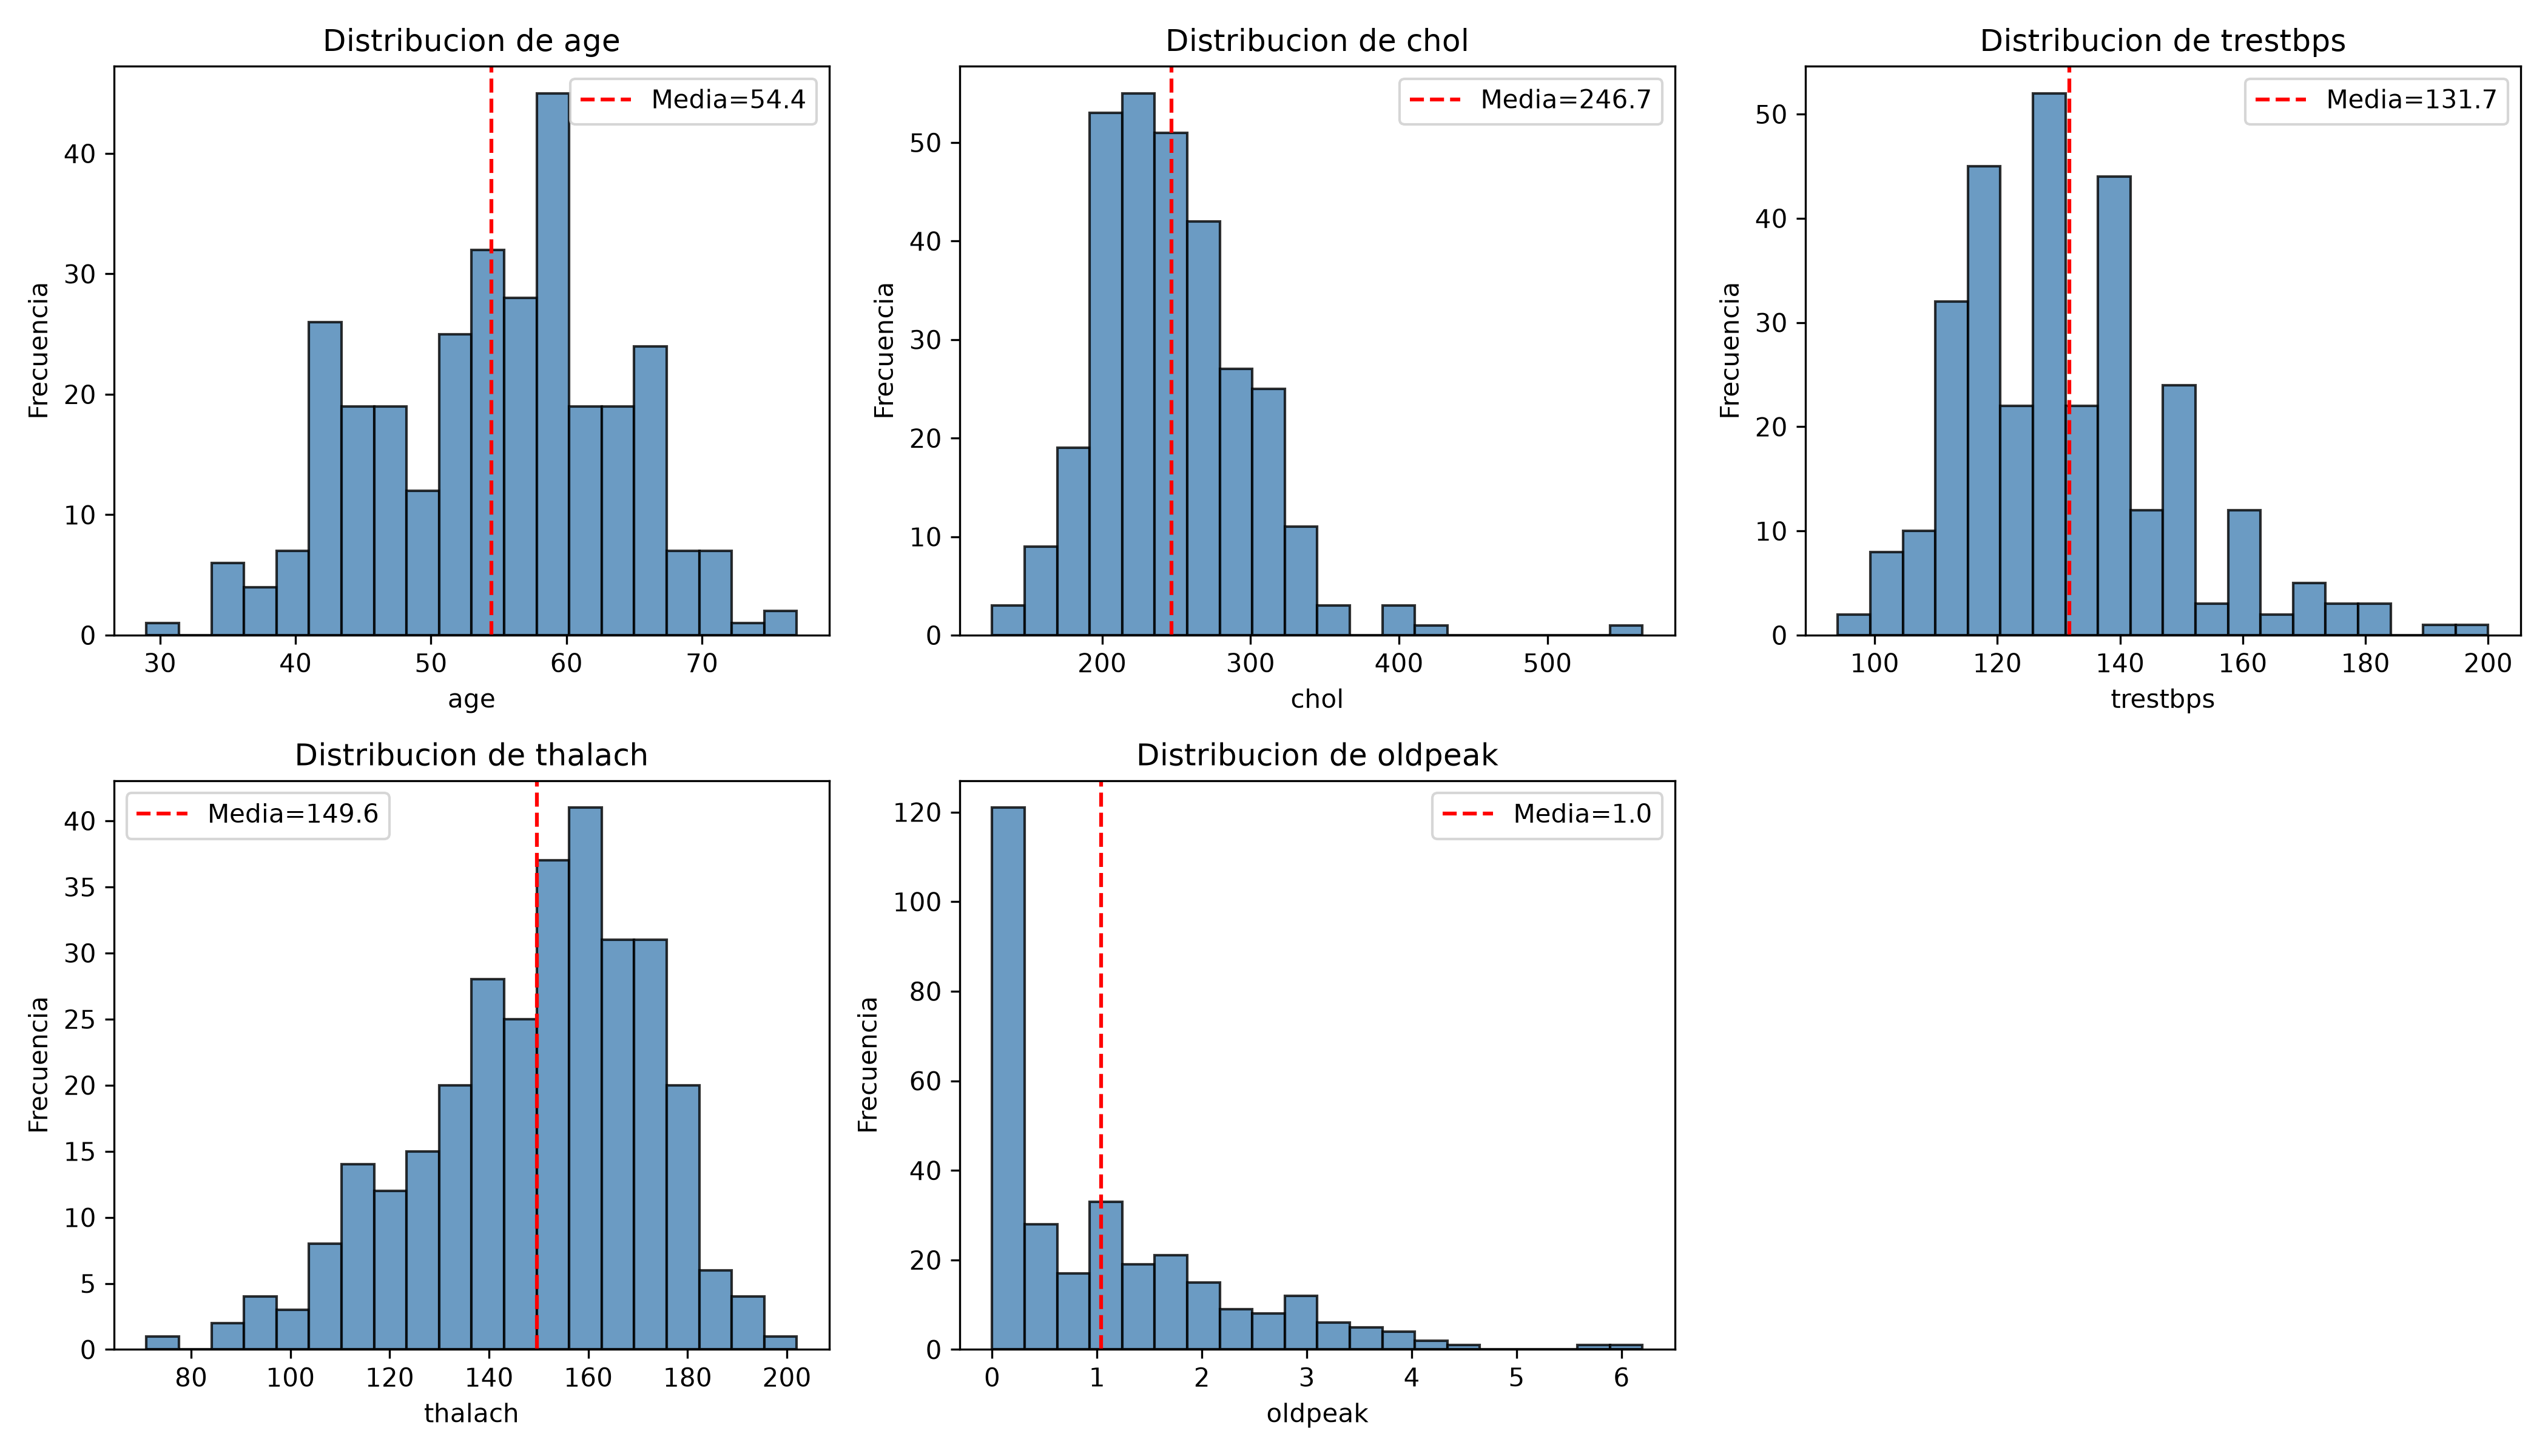
\includegraphics[width=0.85\linewidth]{histogramas.png}
  \caption{Histogramas de las variables críticas con la media marcada.}
  \label{fig:histogramas}
\end{figure}

\begin{figure}[H]
  \centering
  \begin{minipage}{0.48\linewidth}
    \centering
    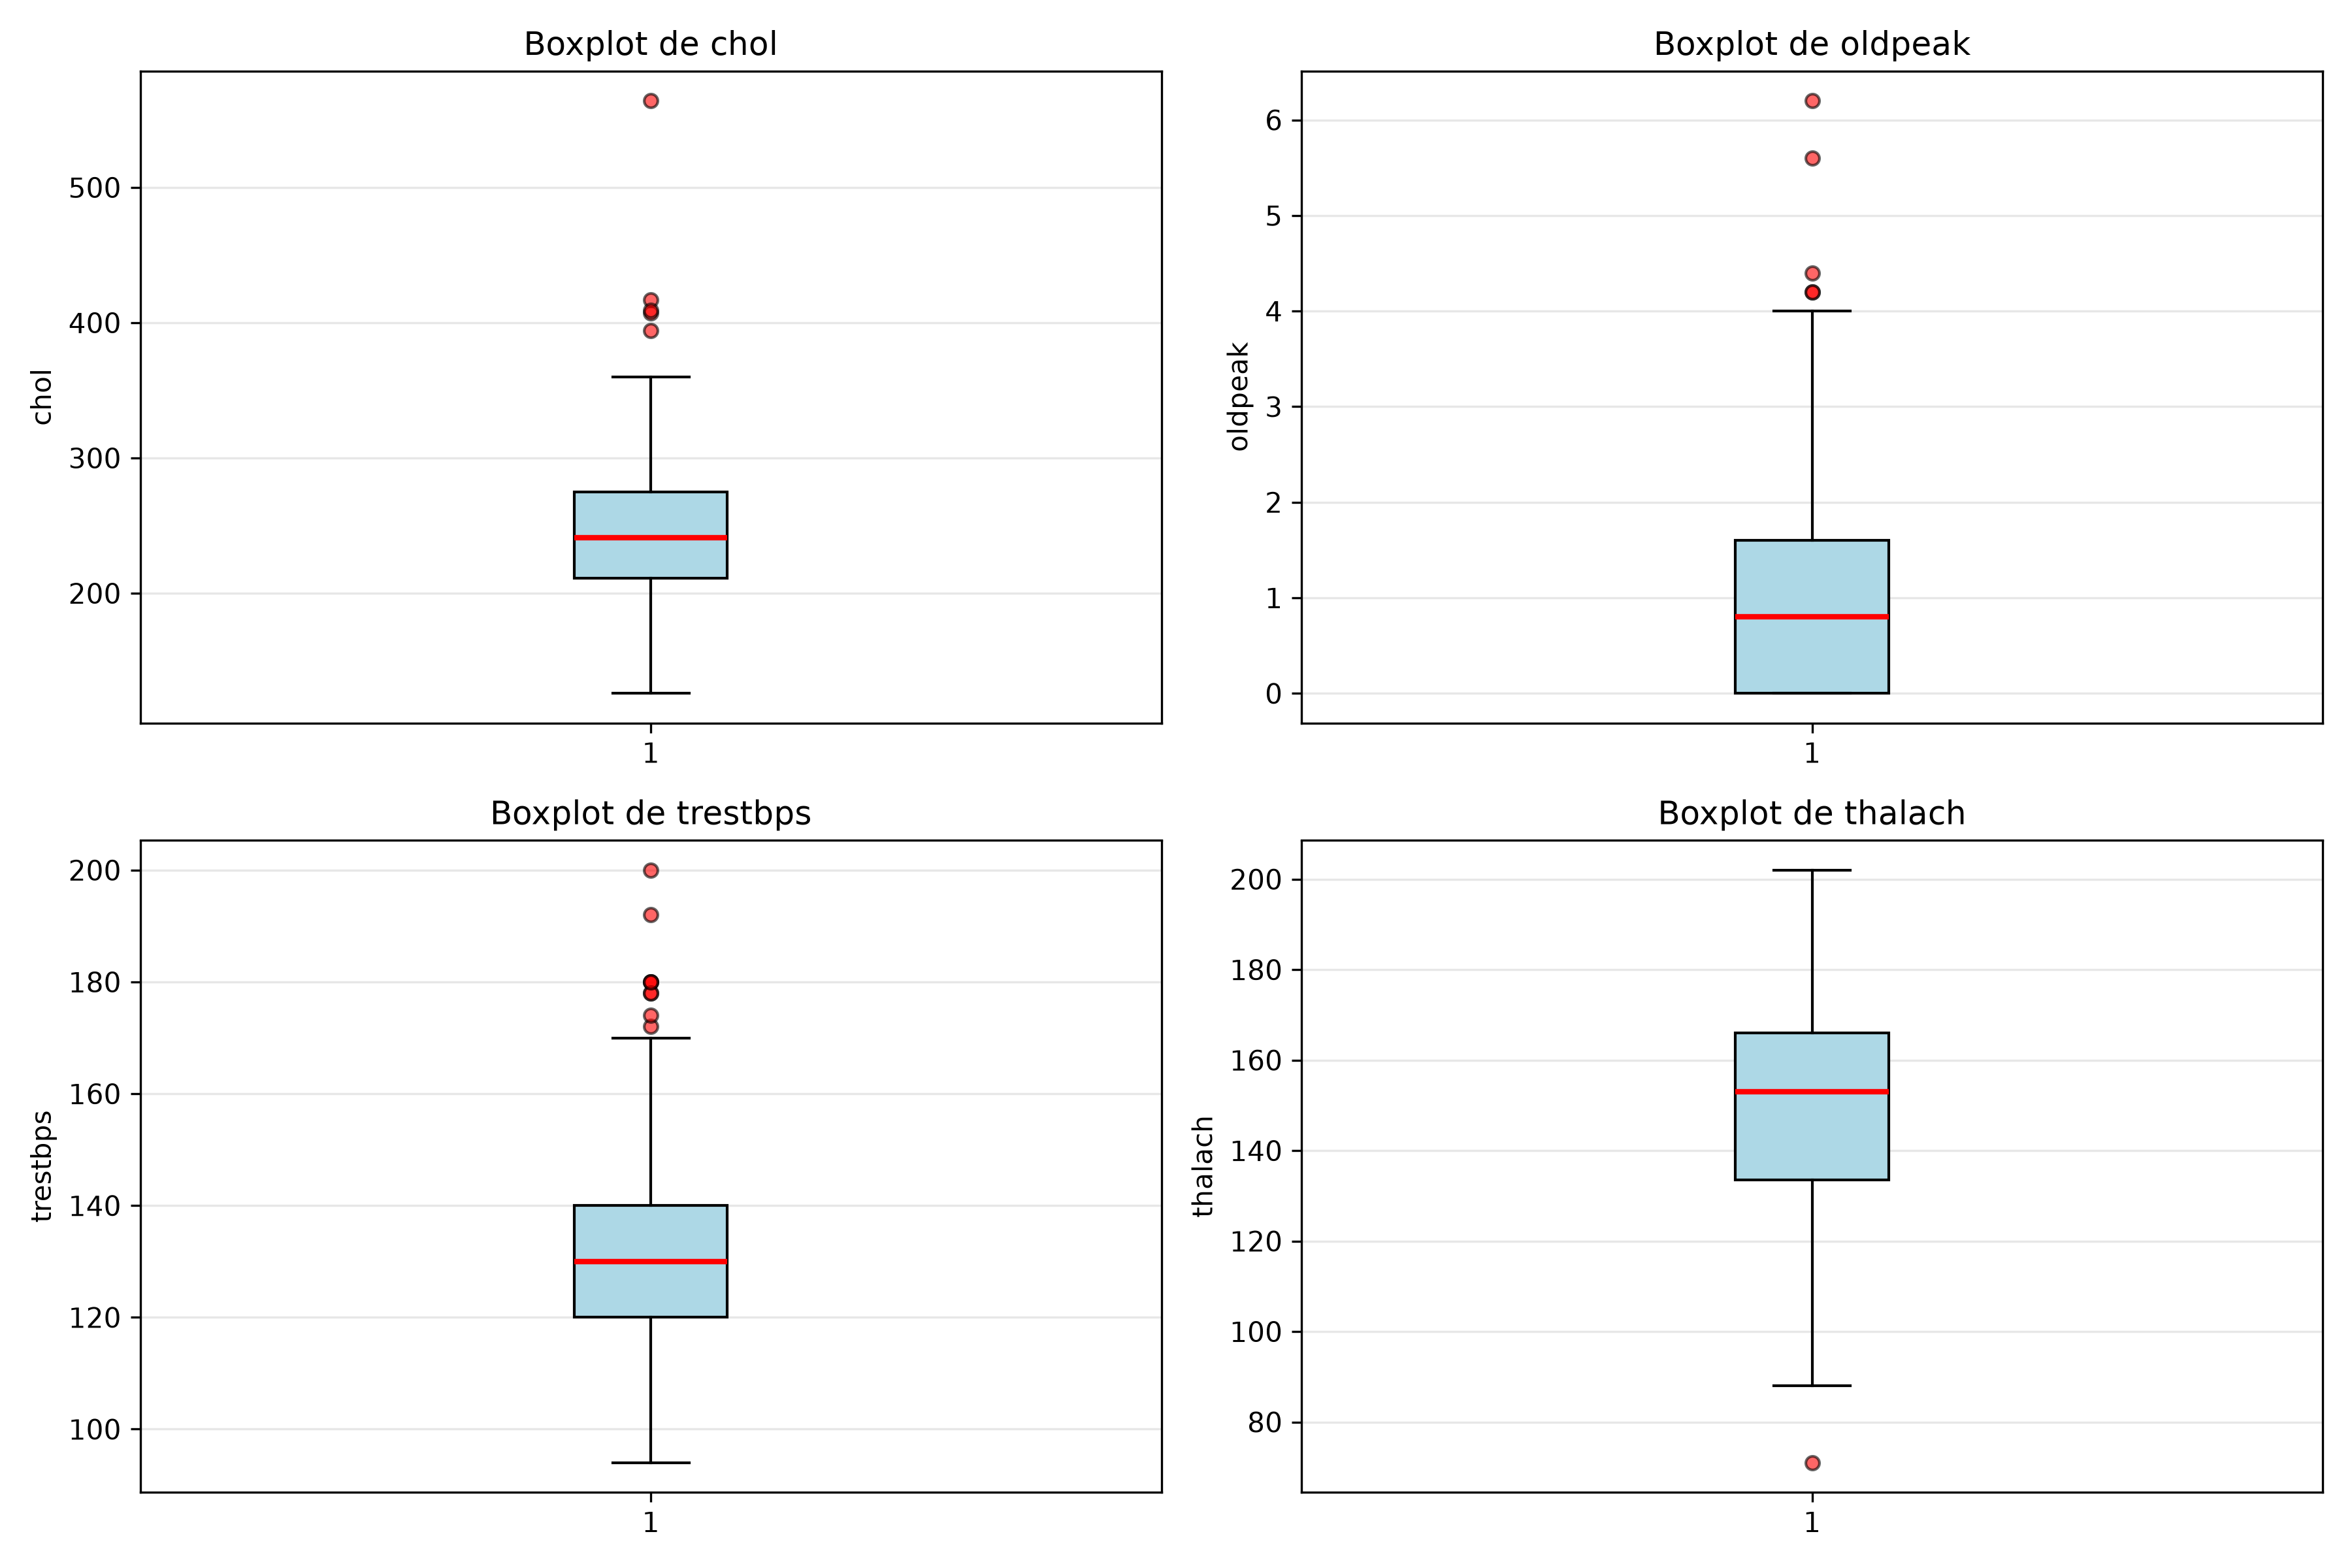
\includegraphics[width=\linewidth]{boxplots.png}
    \caption{Boxplots individuales.}
    \label{fig:boxplots}
  \end{minipage}
  \hfill
  \begin{minipage}{0.48\linewidth}
    \centering
    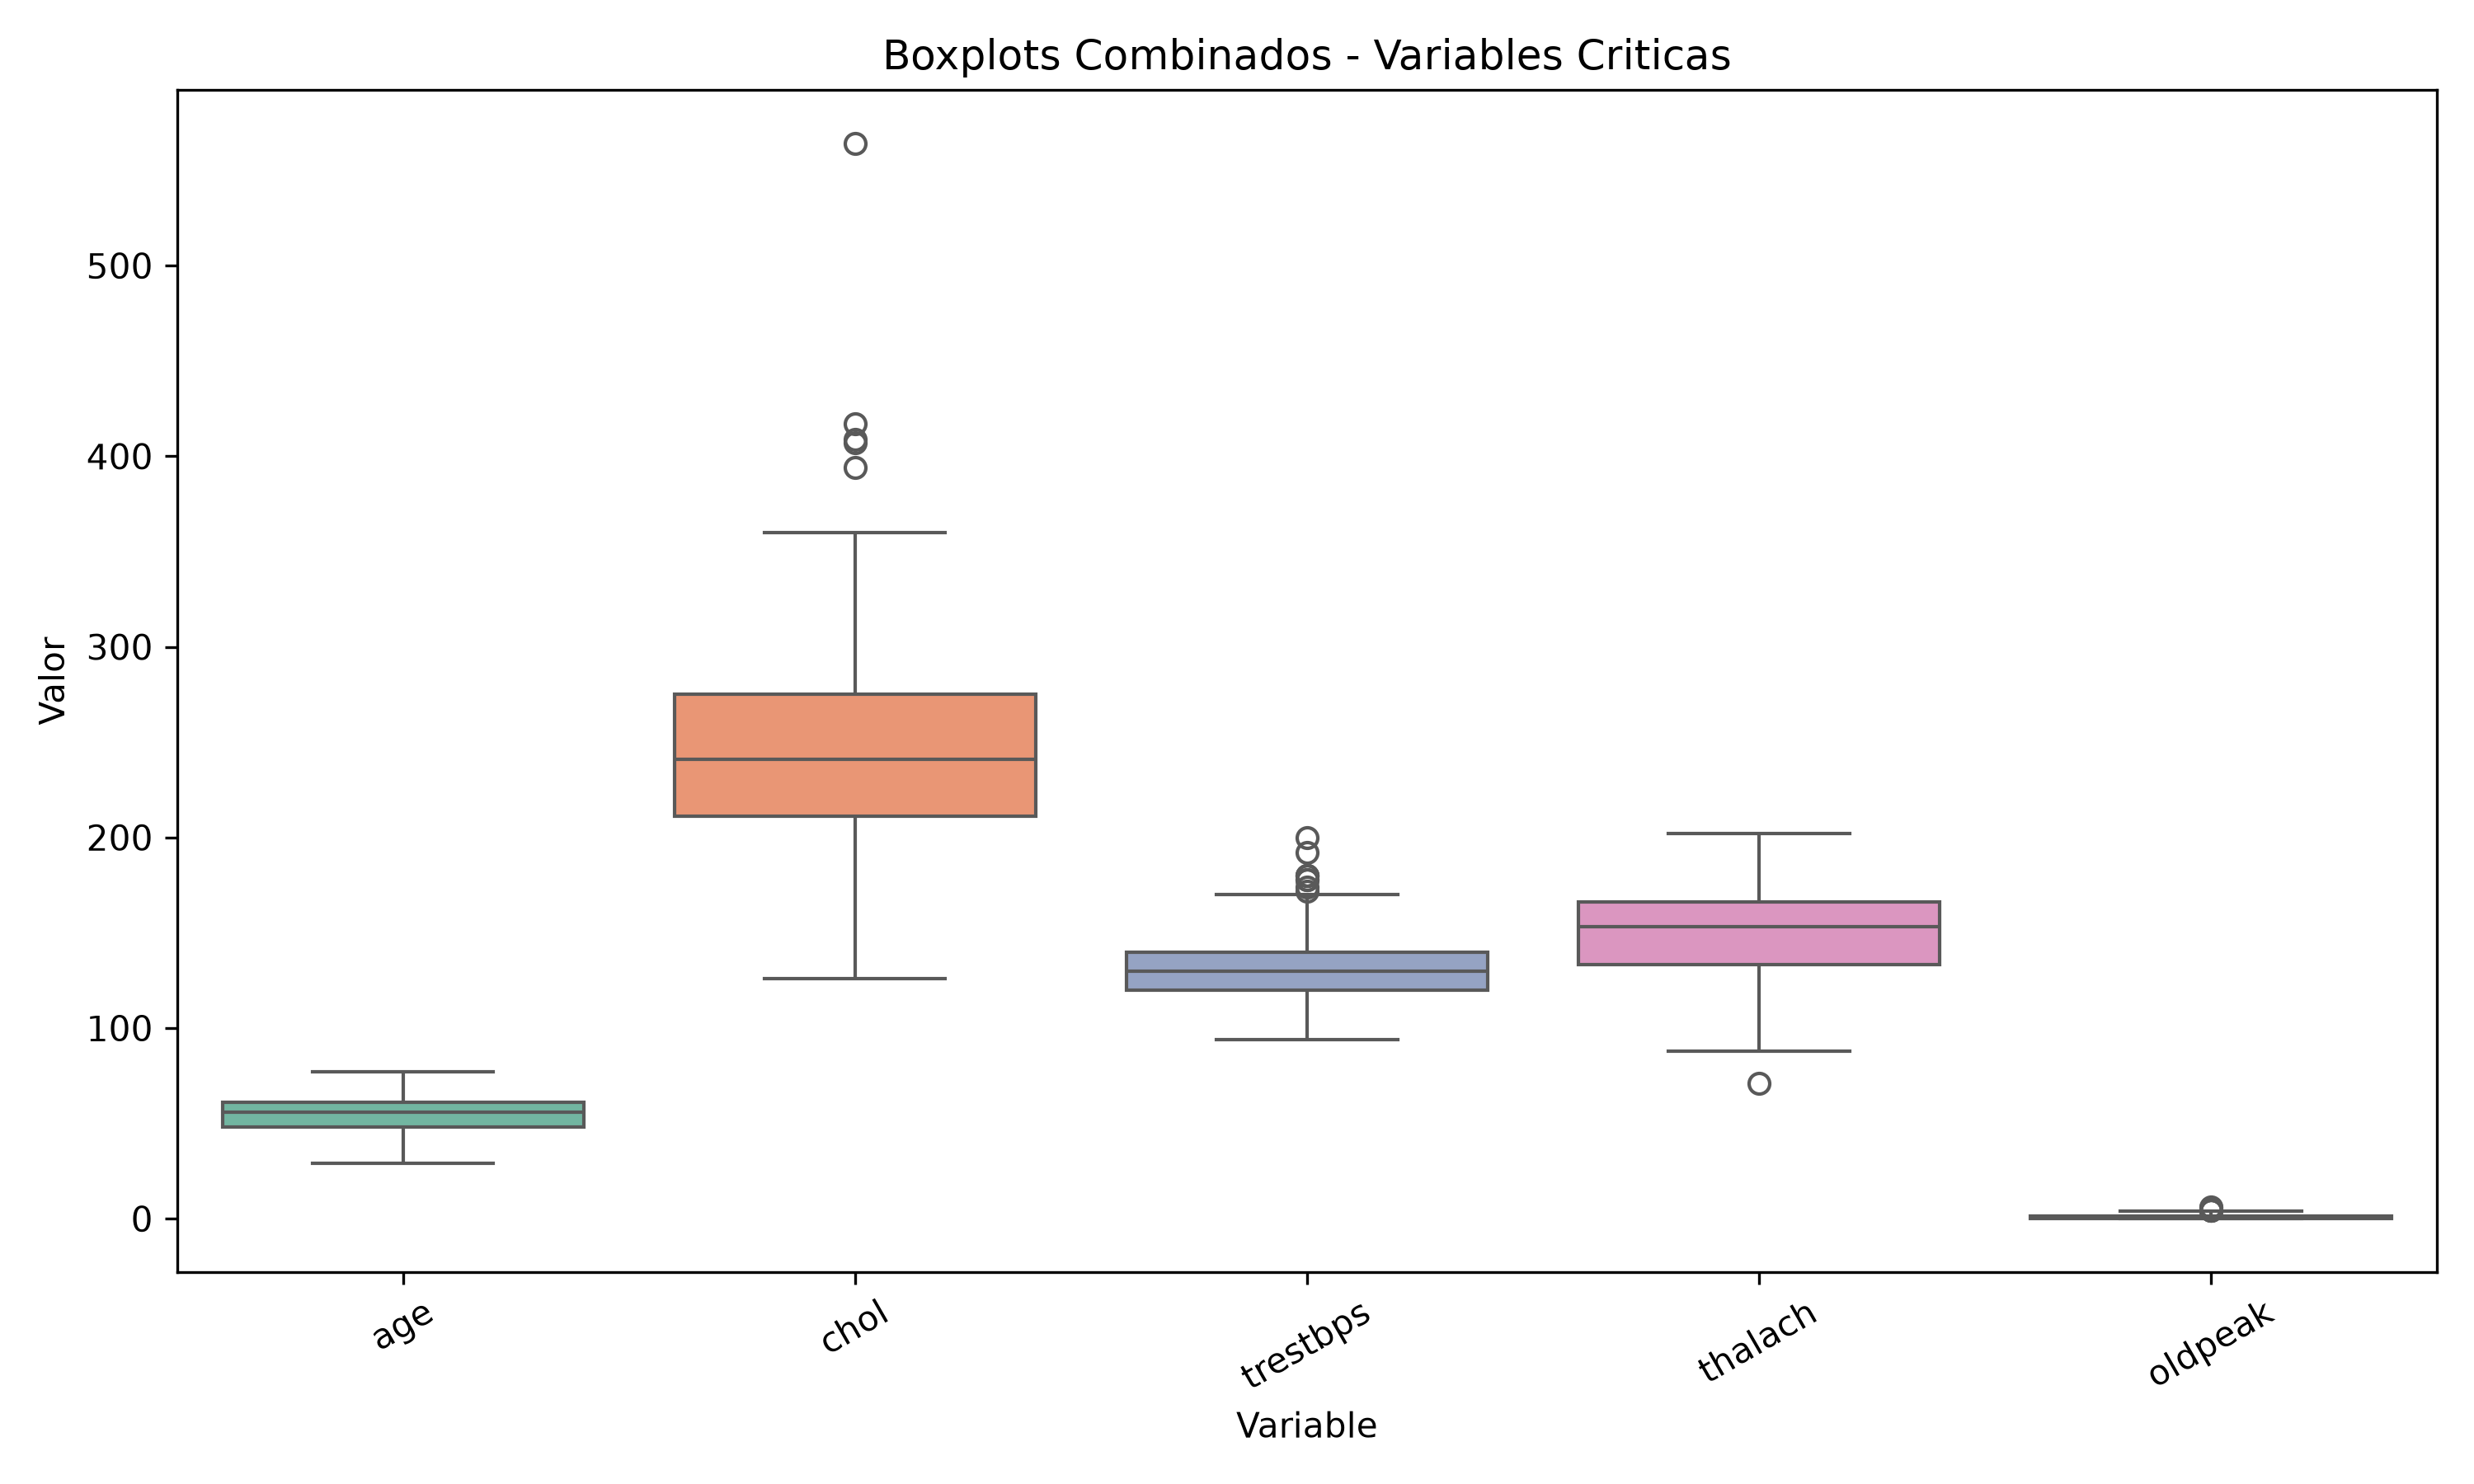
\includegraphics[width=\linewidth]{boxplots_combinados.png}
    \caption{Boxplots combinados.}
    \label{fig:boxplots_combinados}
  \end{minipage}
\end{figure}

\begin{figure}[H]
  \centering
  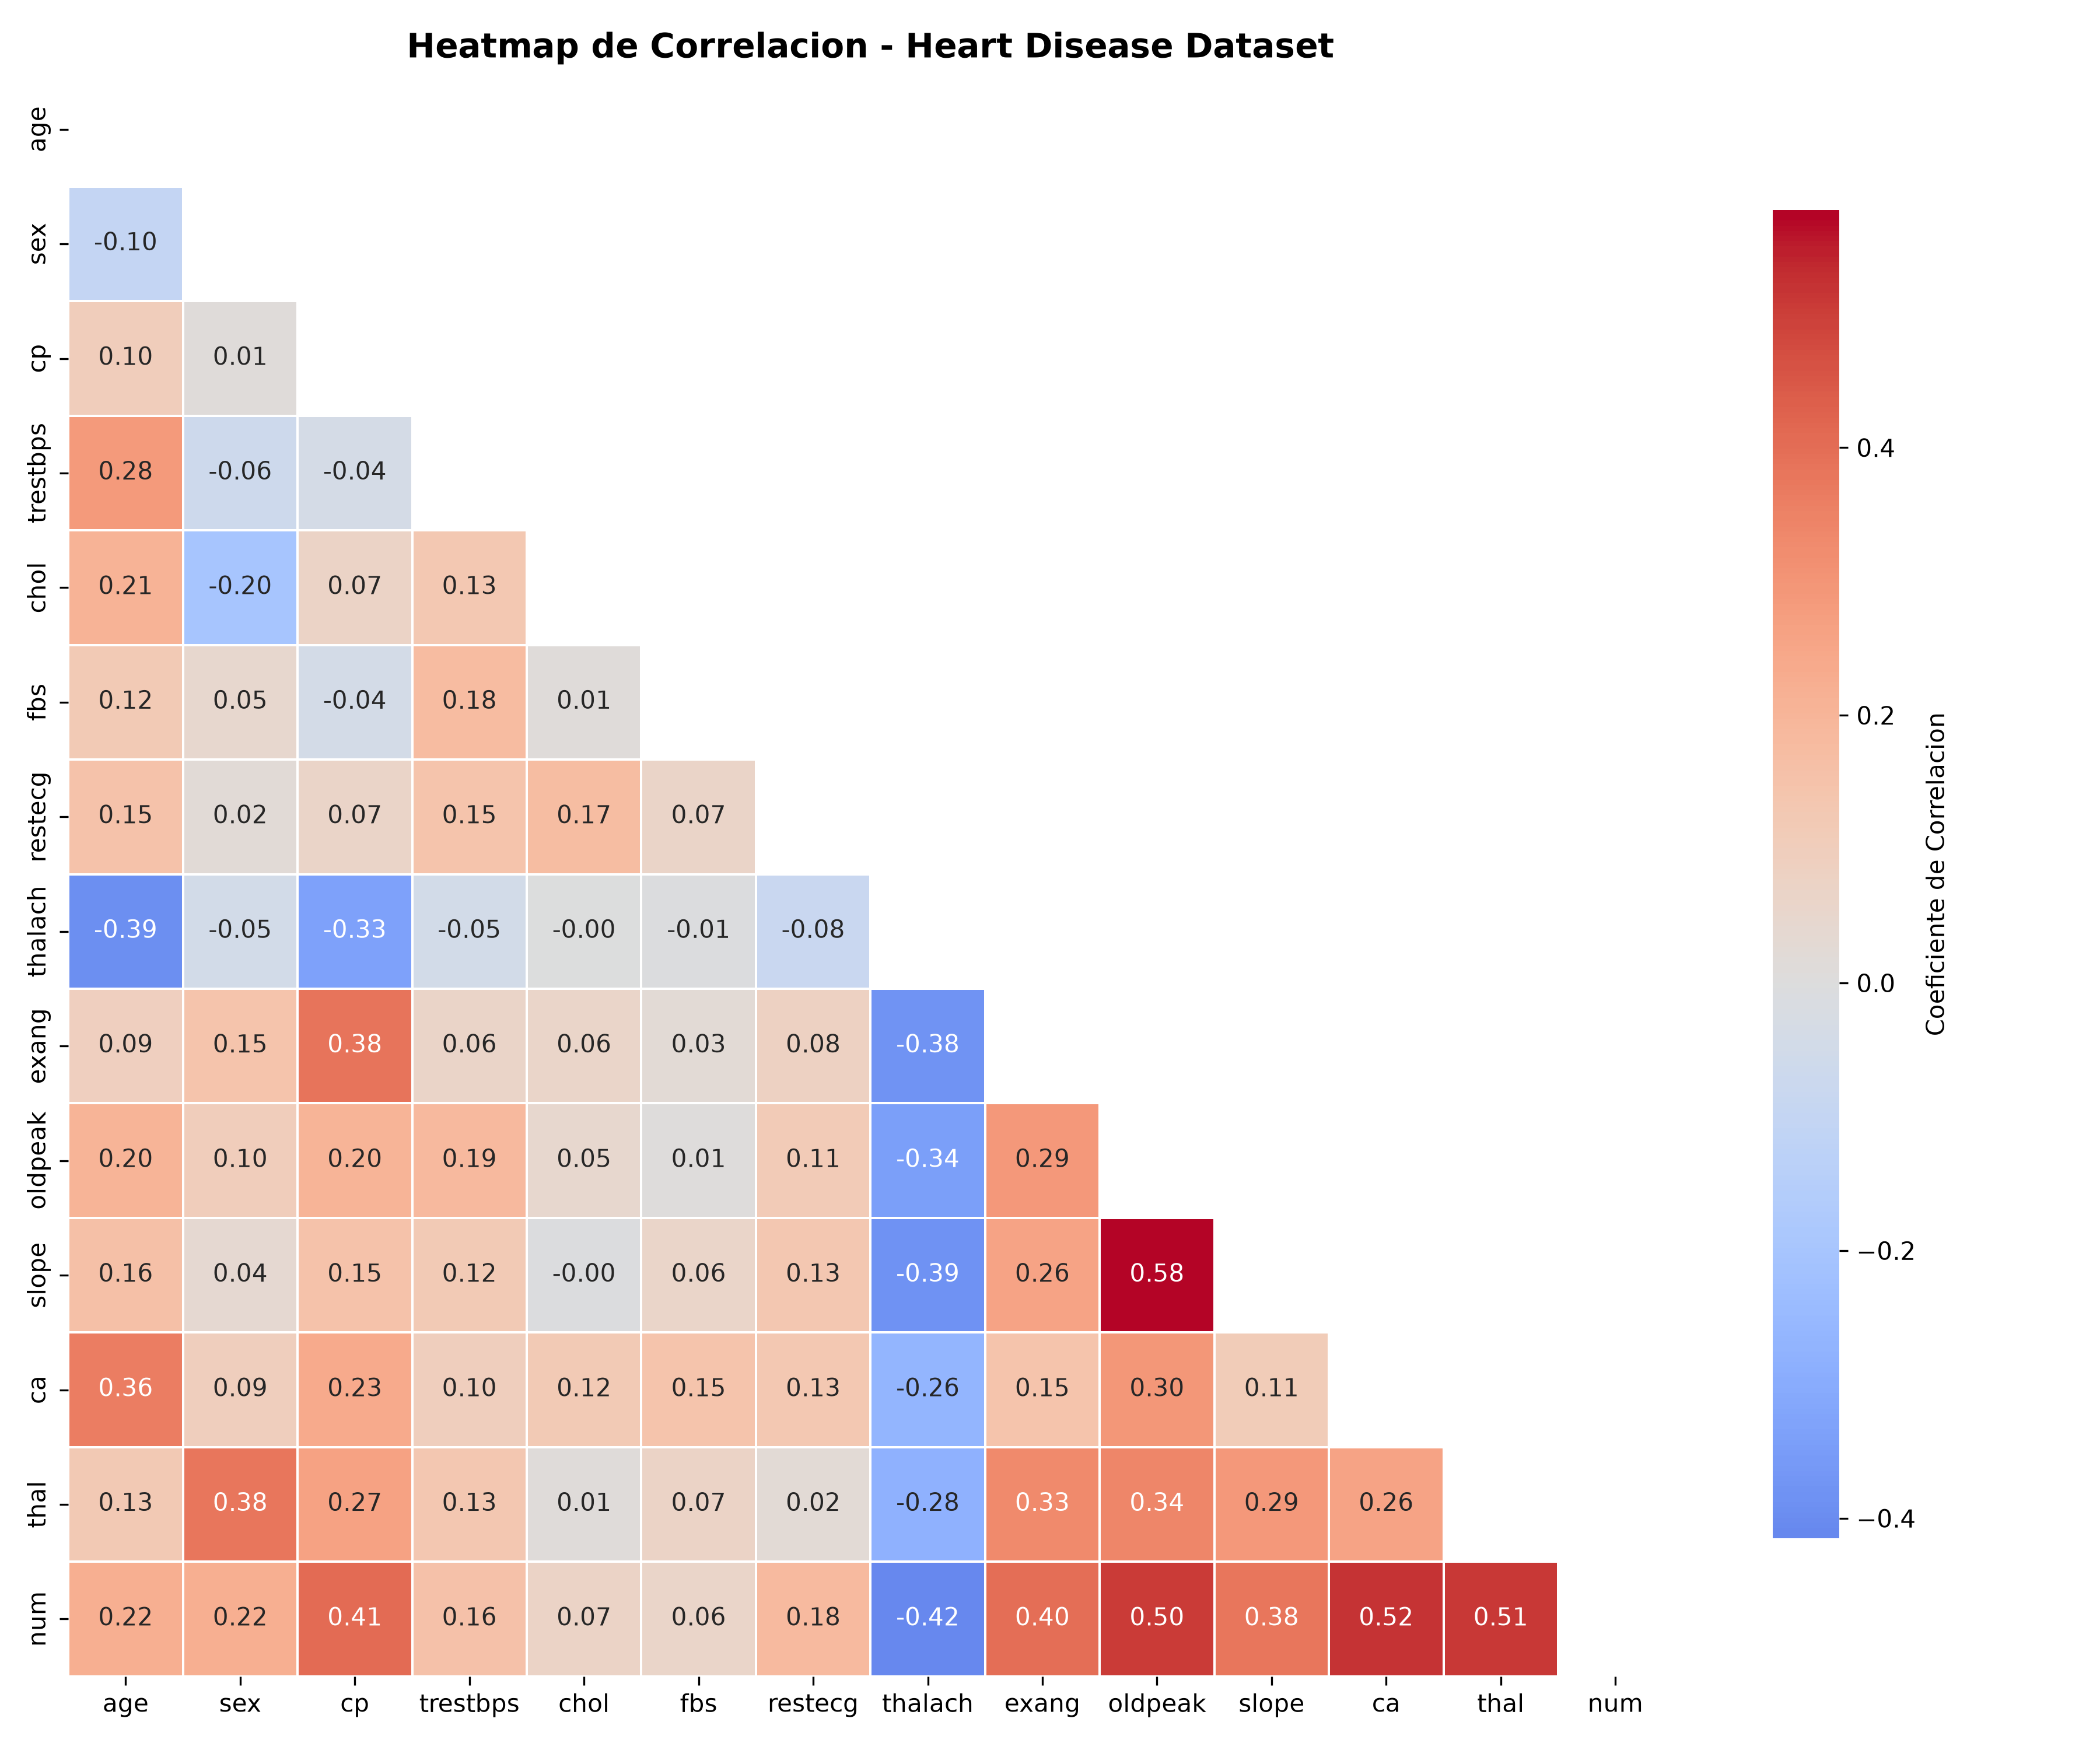
\includegraphics[width=0.75\linewidth]{heatmap_correlacion.png}
  \caption{Heatmap de correlación de Pearson.}
  \label{fig:heatmap}
\end{figure}

\subsection{Preprocesamiento}

\begin{figure}[H]
  \centering
  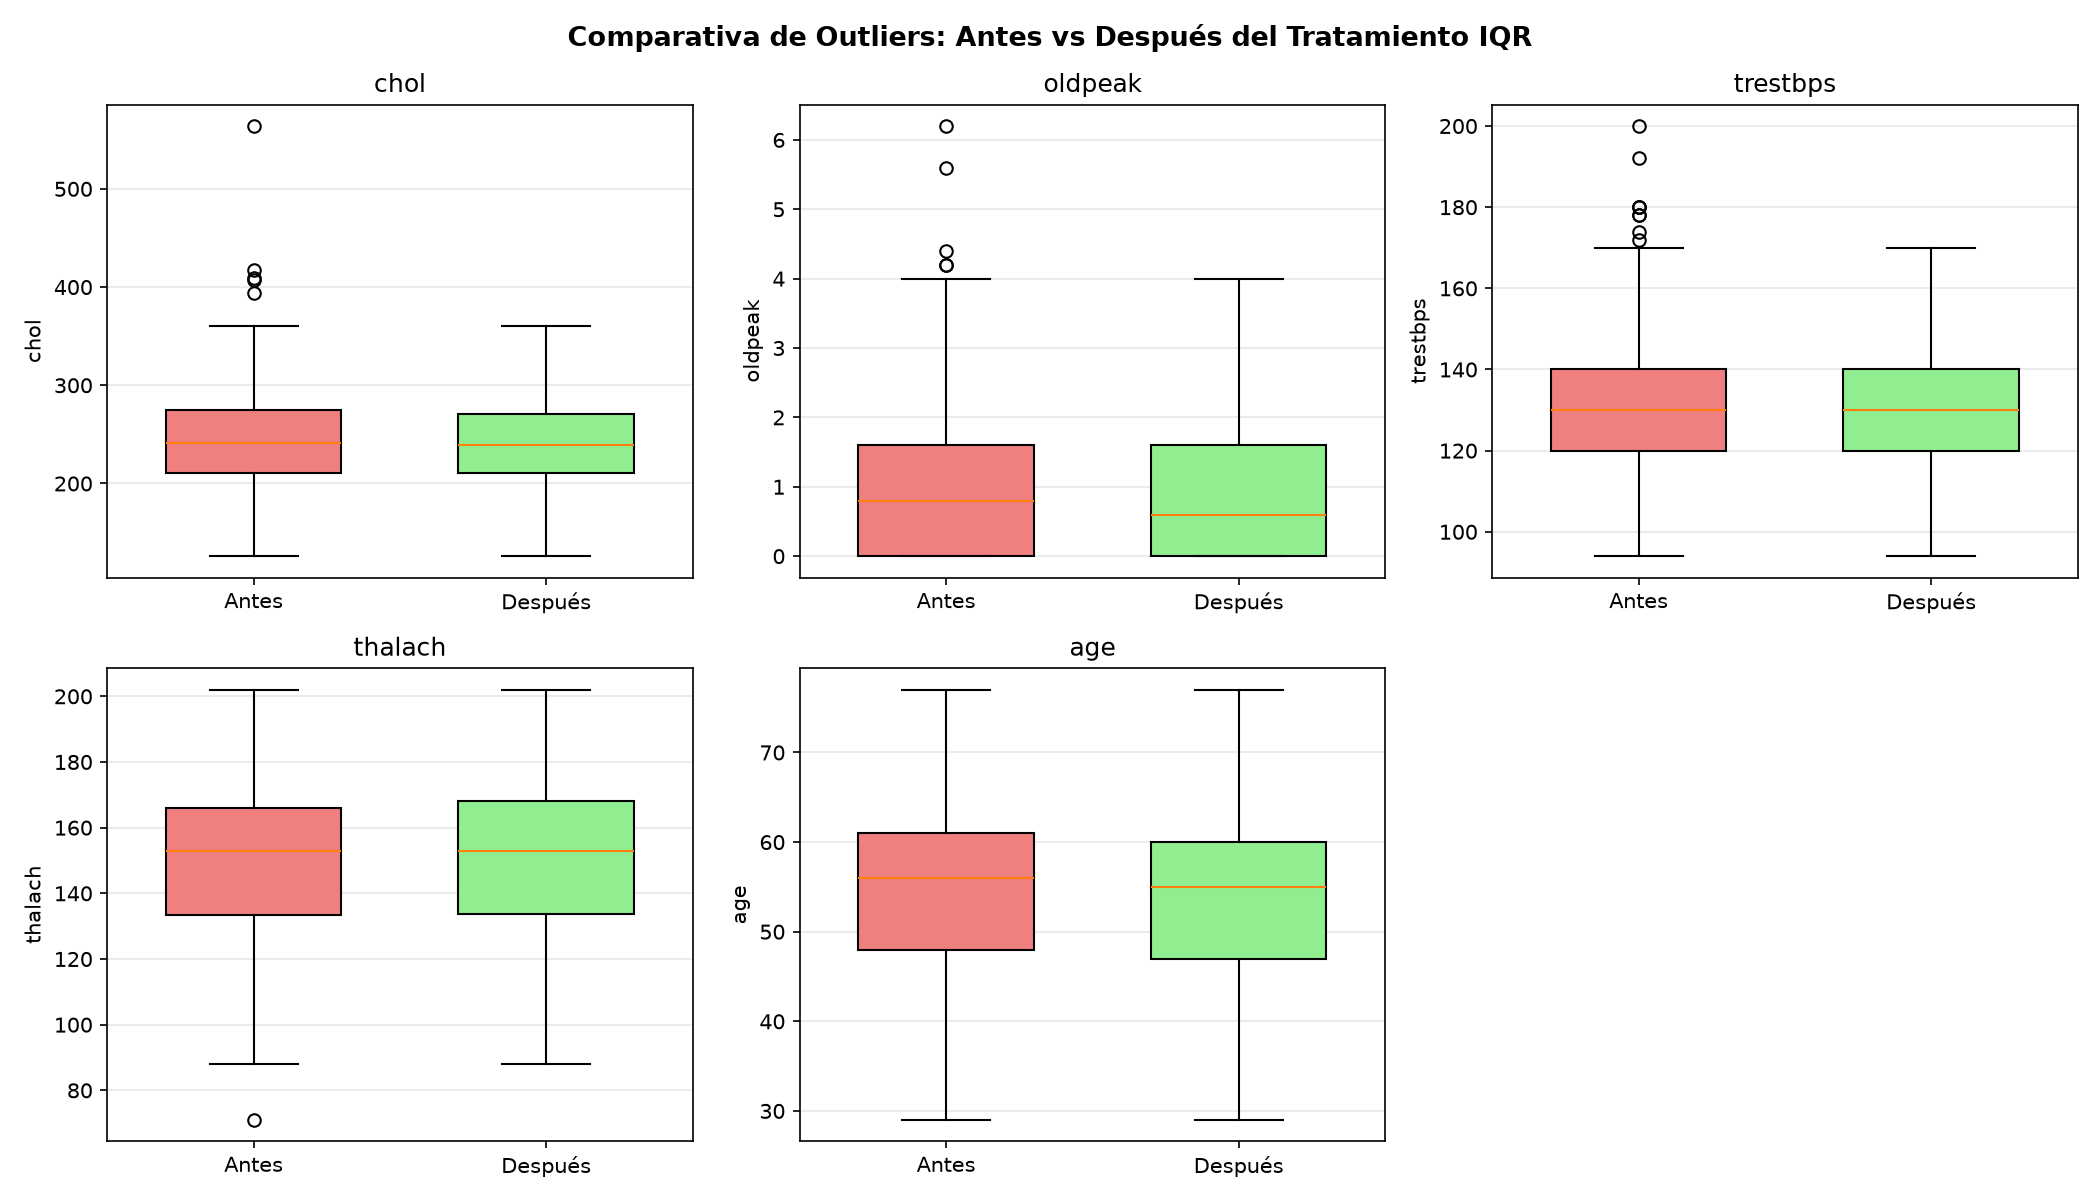
\includegraphics[width=0.75\linewidth]{outliers_antes_despues.png}
  \caption{Comparación antes/después de la eliminación de outliers (IQR).}
  \label{fig:outliers}
\end{figure}

\subsection{Reducción de dimensionalidad}

\begin{figure}[H]
  \centering
  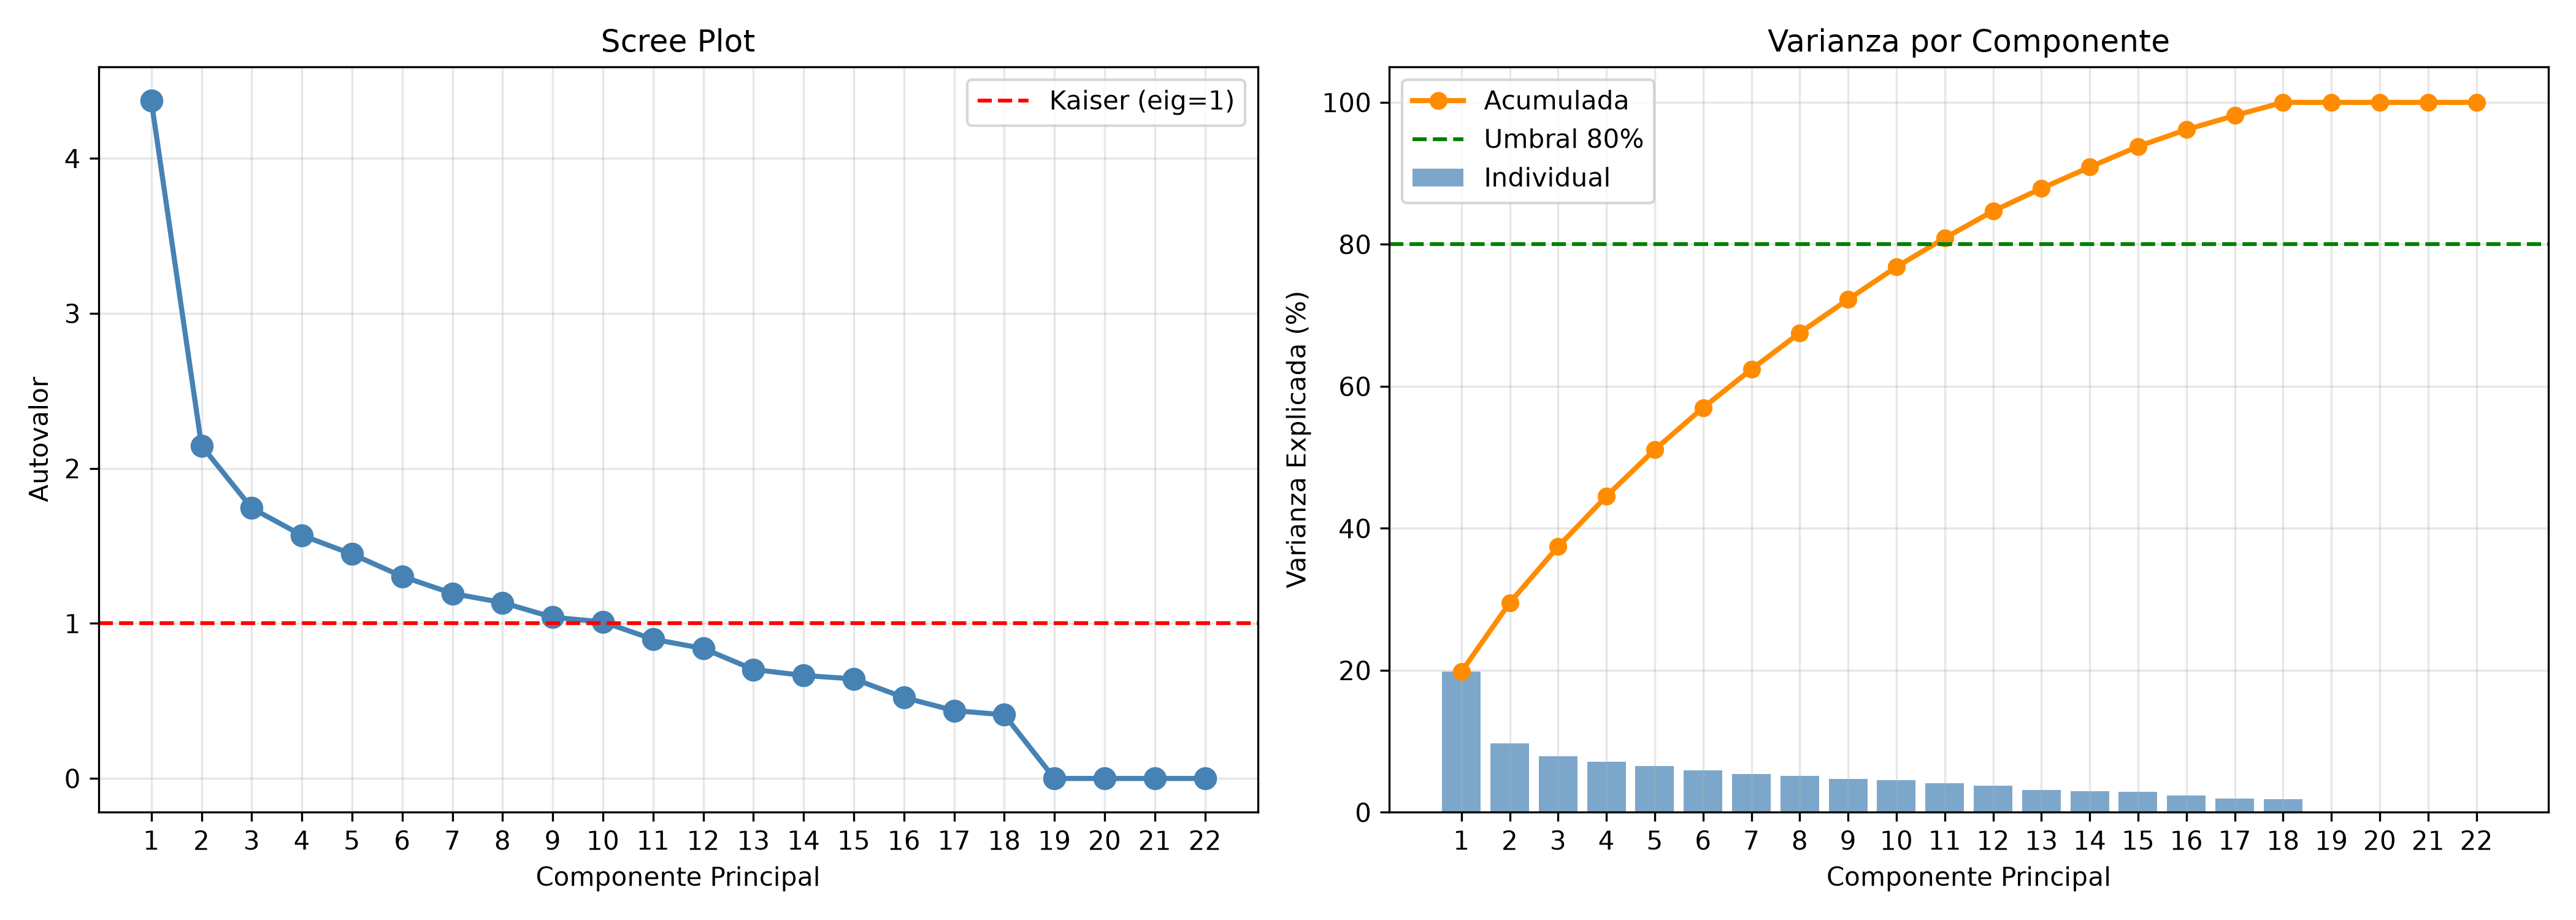
\includegraphics[width=0.85\linewidth]{pca_varianza.png}
  \caption{PCA: scree plot (autovalores) y varianza explicada individual y acumulada.}
  \label{fig:pca_varianza}
\end{figure}

\begin{figure}[H]
  \centering
  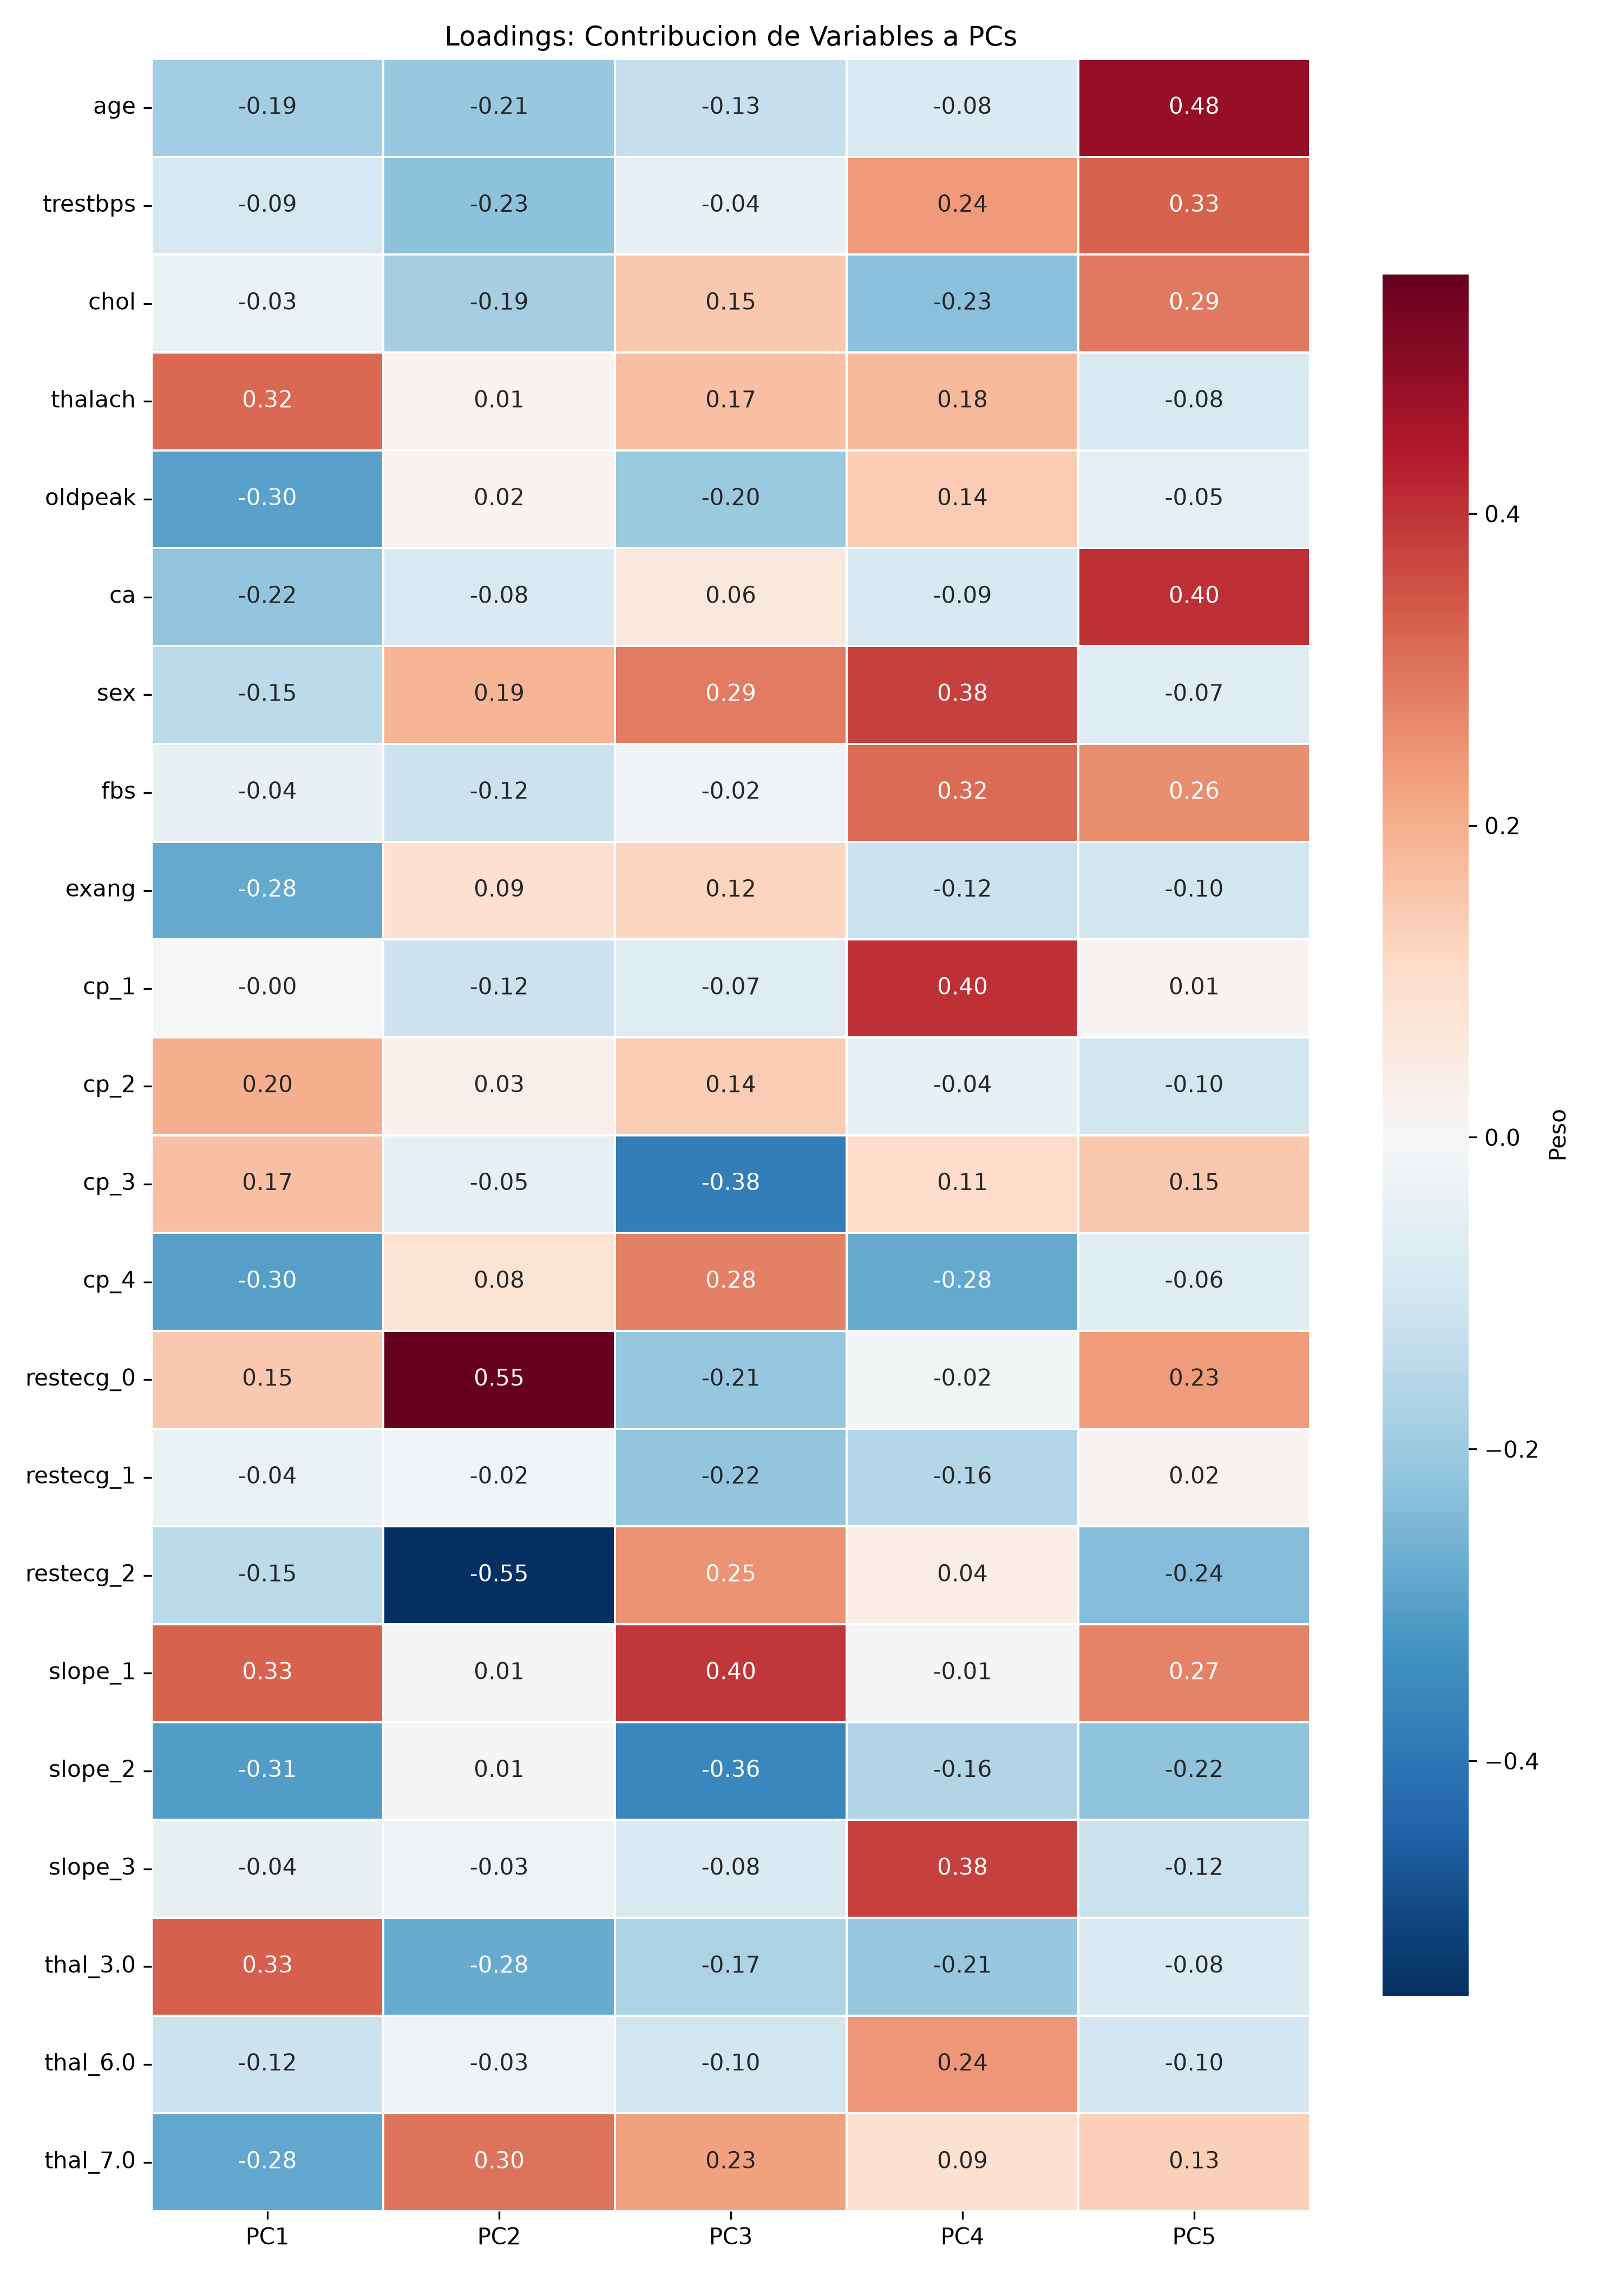
\includegraphics[width=0.62\linewidth]{pca_loadings.png}
  \caption{Heatmap de loadings (PC1--PC5).}
  \label{fig:pca_loadings}
\end{figure}

\begin{figure}[H]
  \centering
  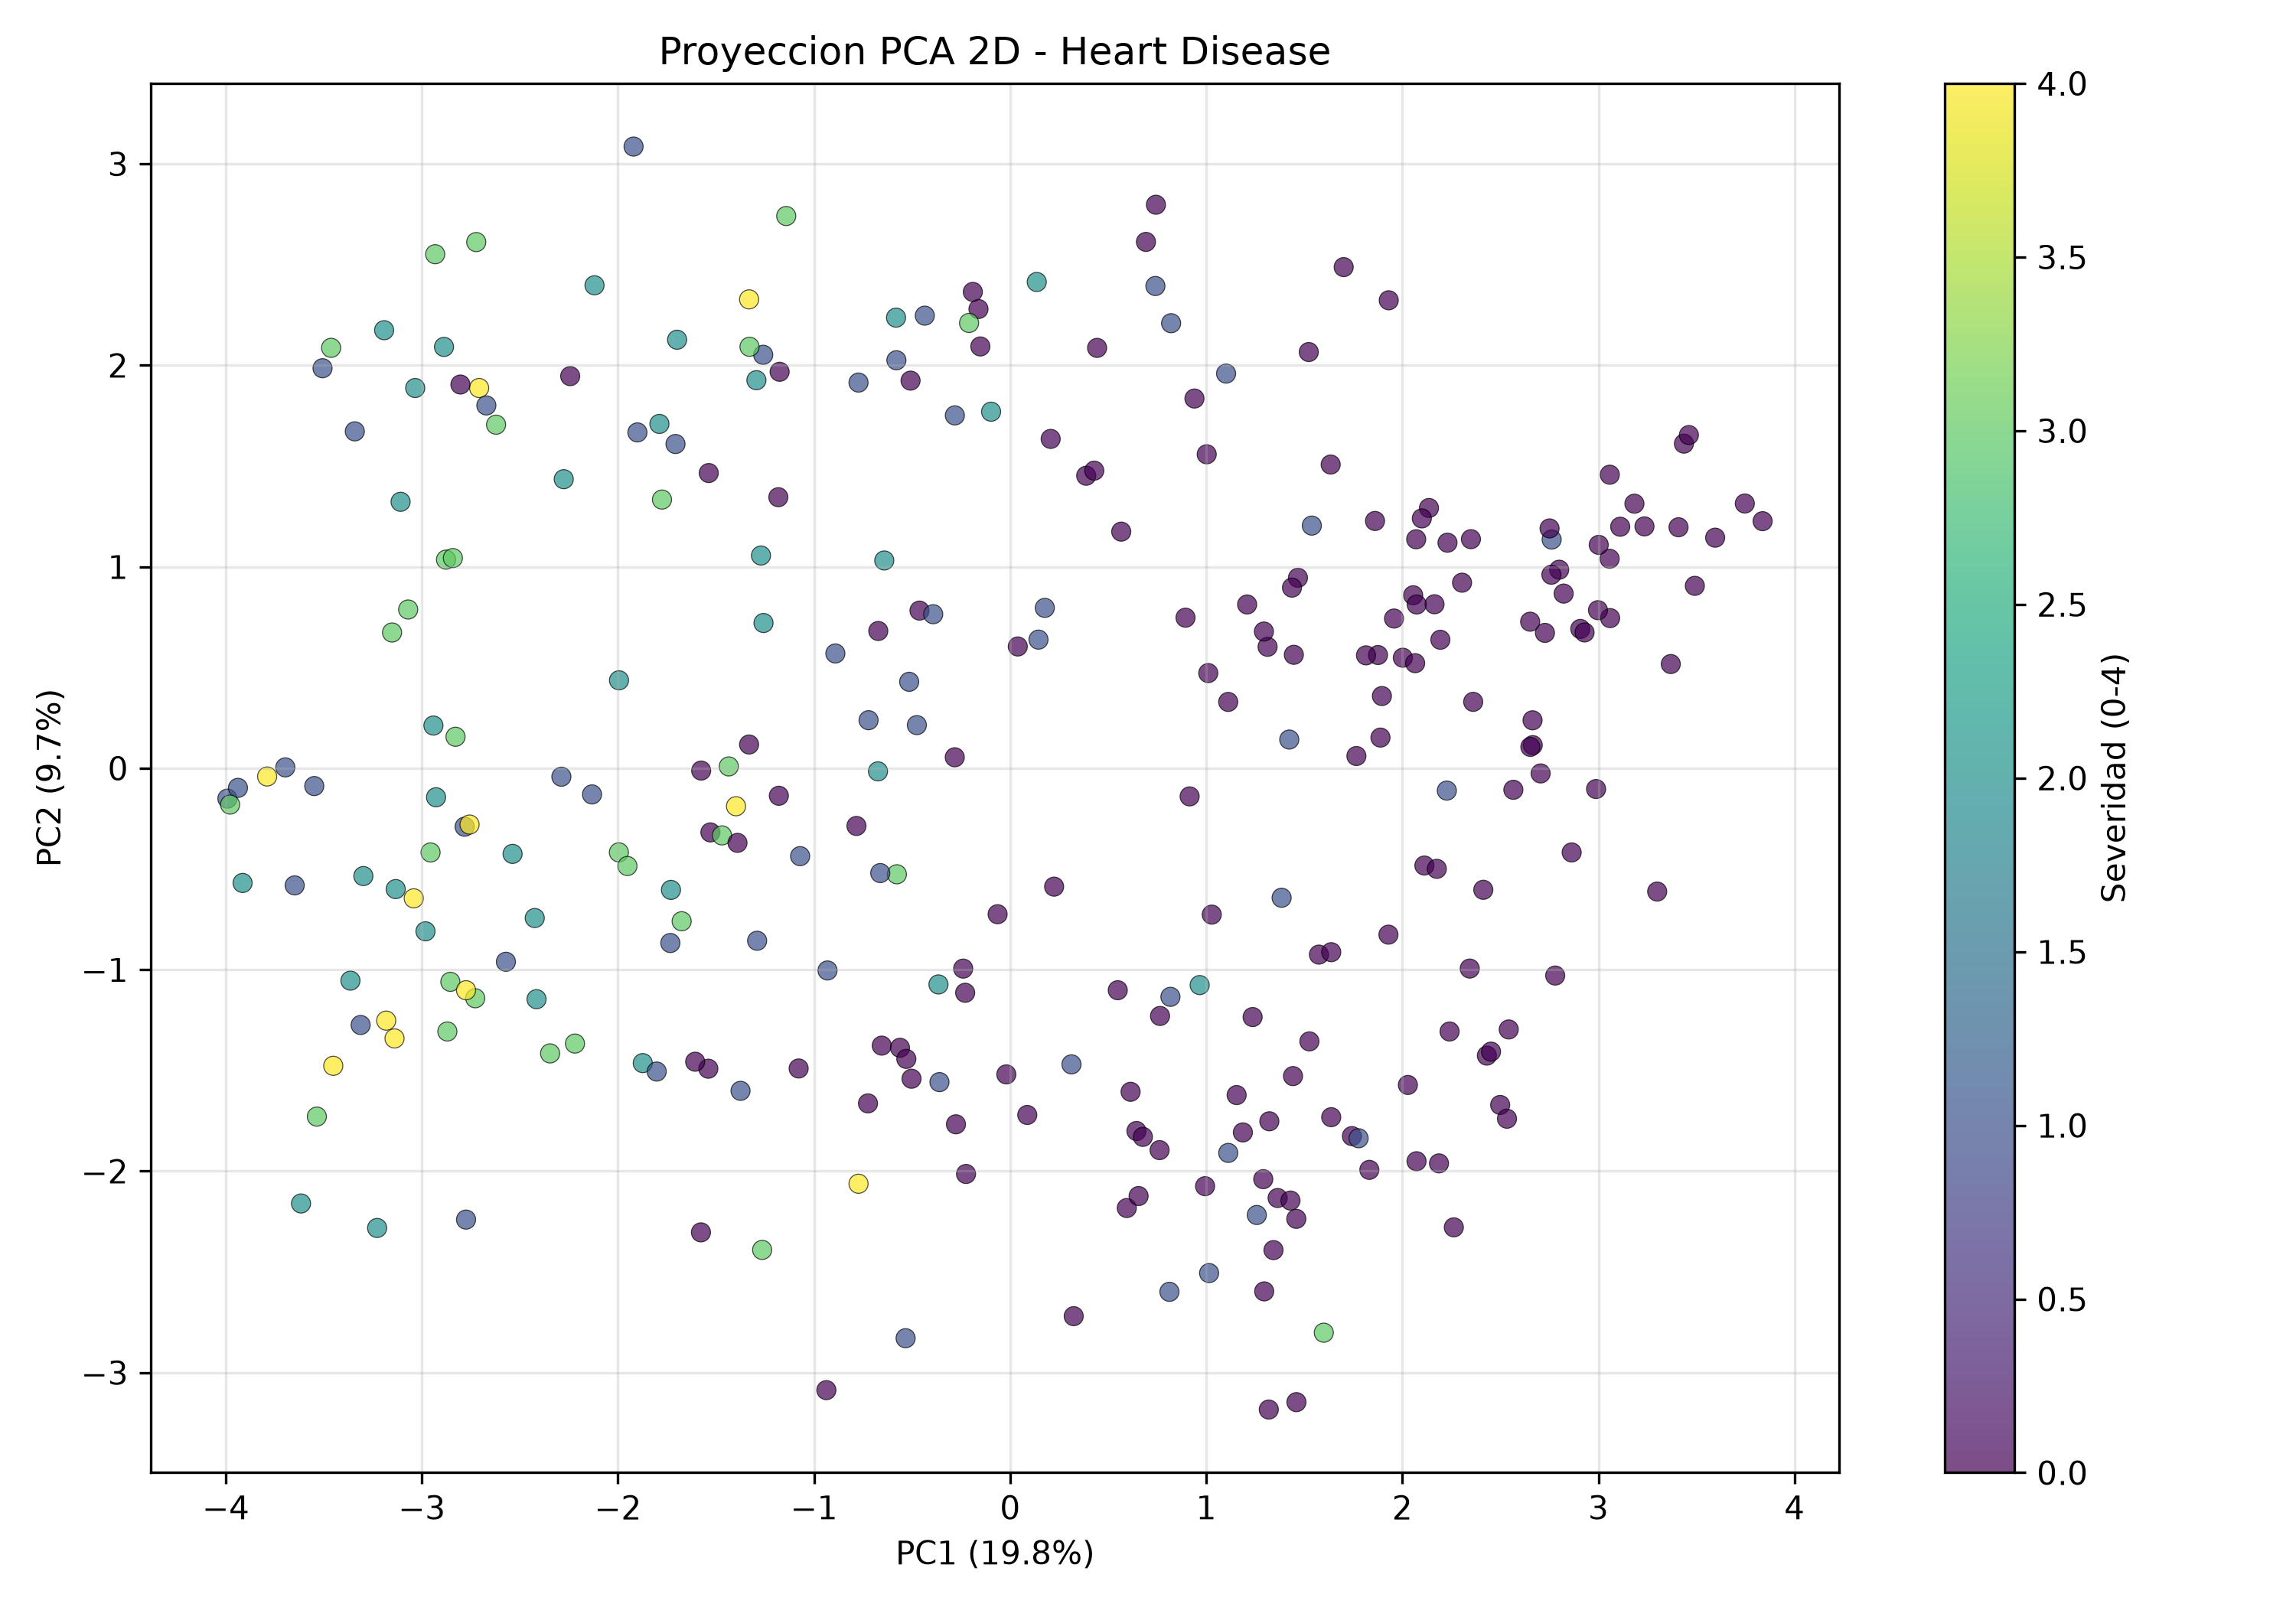
\includegraphics[width=0.7\linewidth]{pca_proyeccion_2d.png}
  \caption{Proyección PCA 2D coloreada por severidad (0--4).}
  \label{fig:pca_proyeccion}
\end{figure}

\begin{figure}[H]
  \centering
  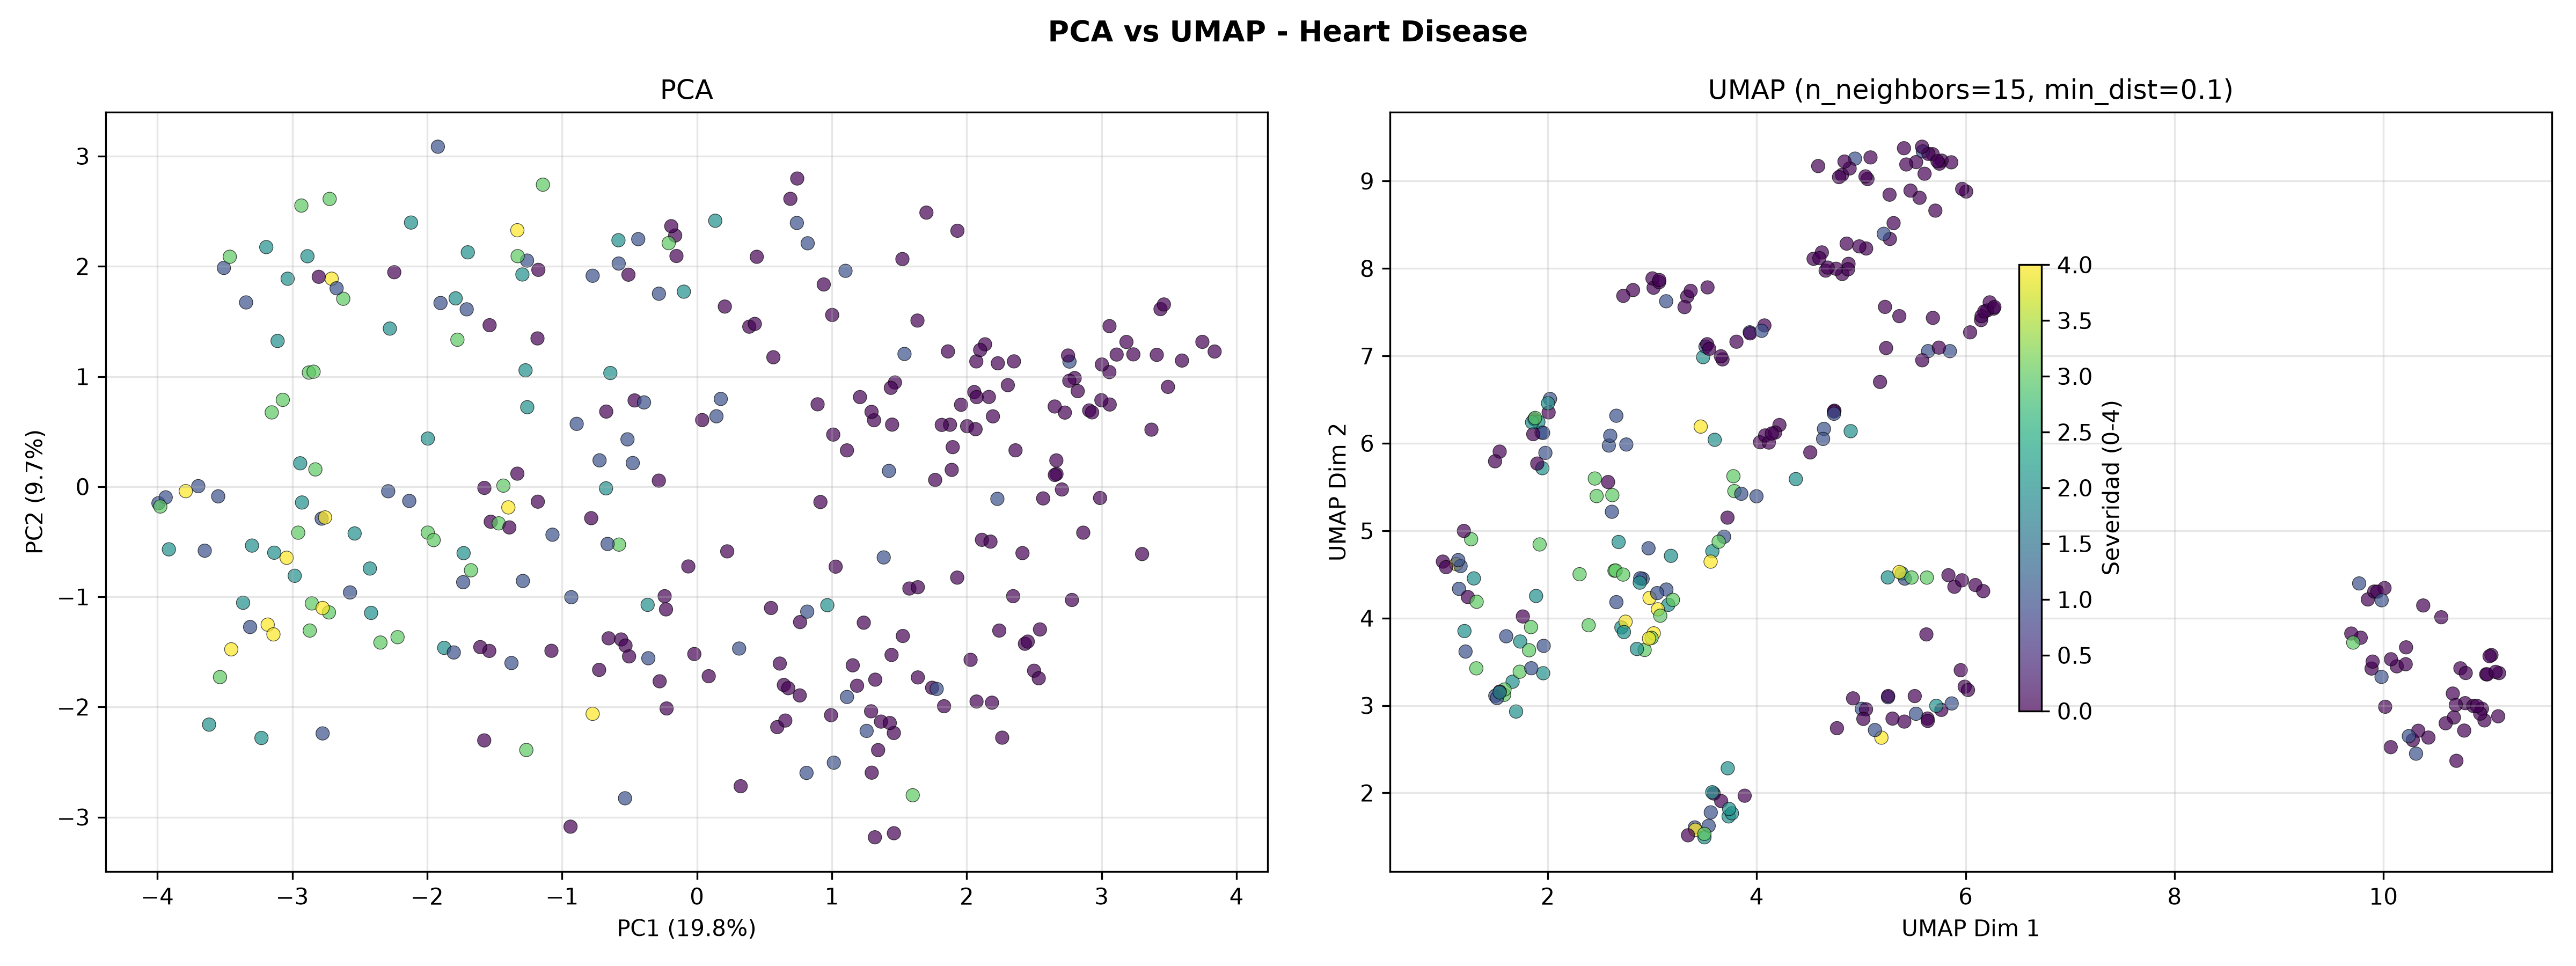
\includegraphics[width=0.9\linewidth]{pca_vs_umap.png}
  \caption{Comparación visual PCA vs. UMAP coloreada por severidad.}
  \label{fig:pca_vs_umap}
\end{figure}

\begin{figure}[H]
  \centering
  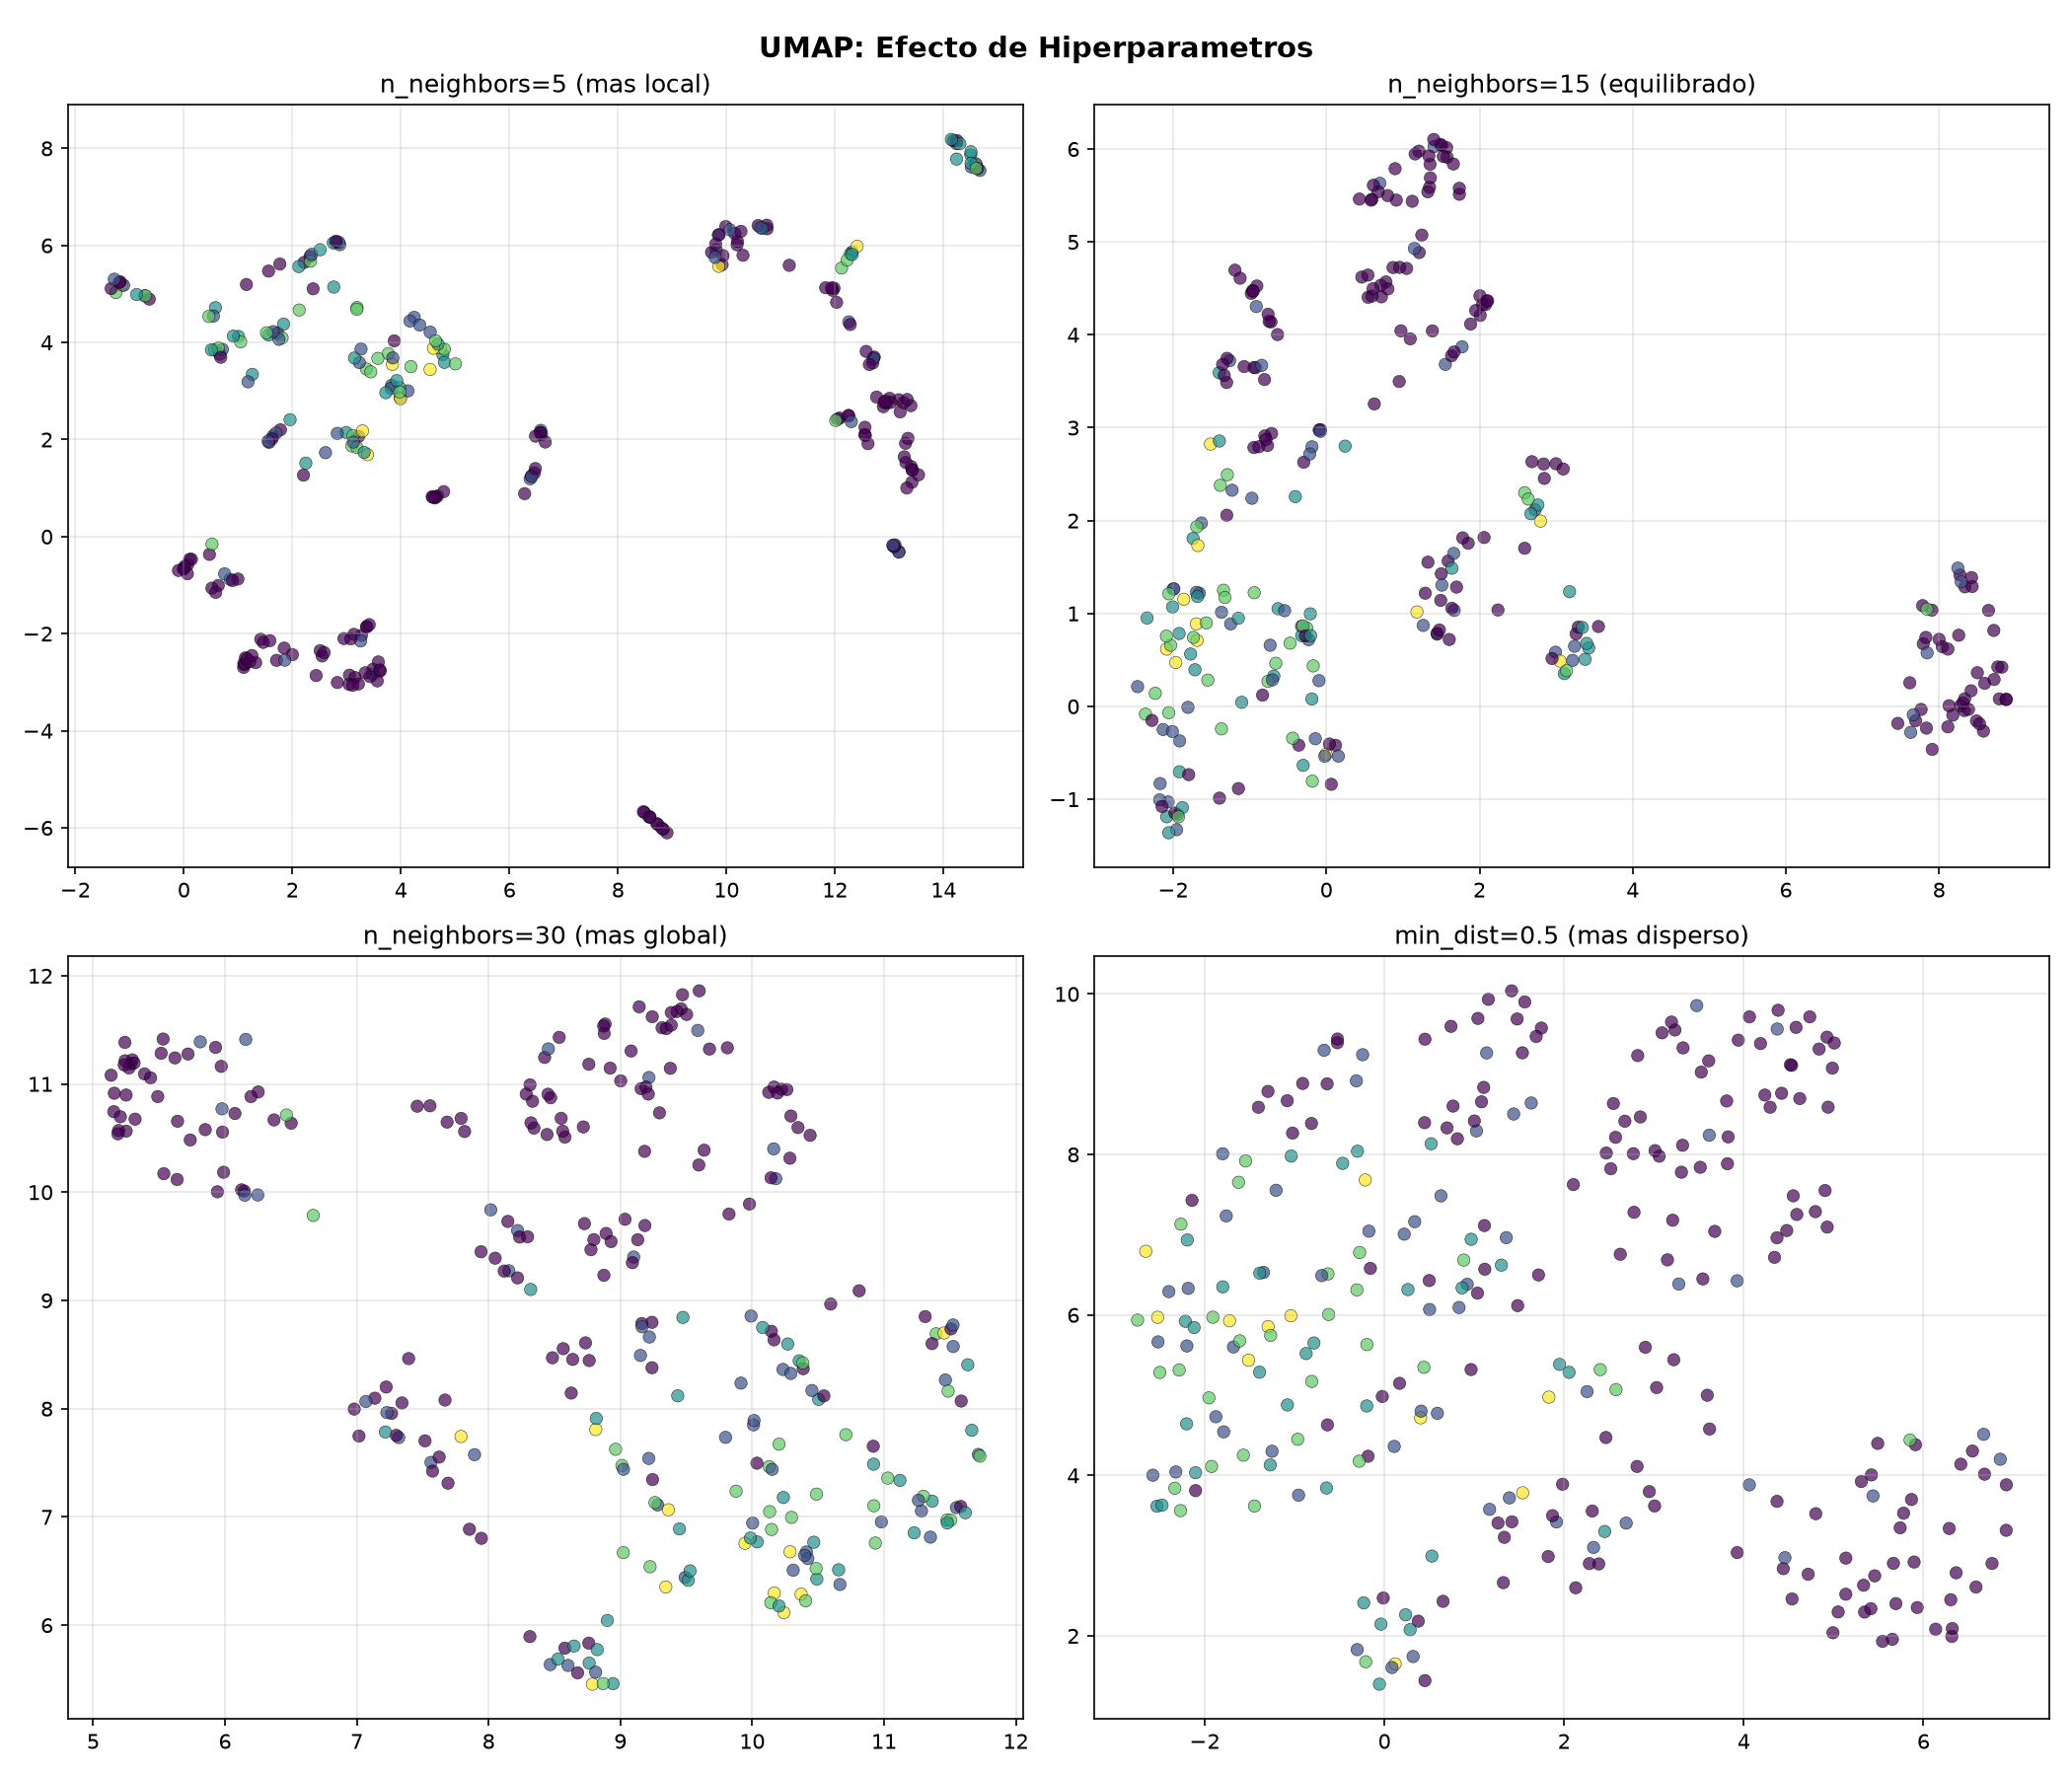
\includegraphics[width=0.85\linewidth]{umap_hiperparametros.png}
  \caption{UMAP: efecto de los hiperparámetros $n\_neighbors$ y $min\_dist$.}
  \label{fig:umap_hiperparametros}
\end{figure}

\subsection{Clustering}

\begin{figure}[H]
  \centering
  \begin{minipage}{0.48\linewidth}
    \centering
    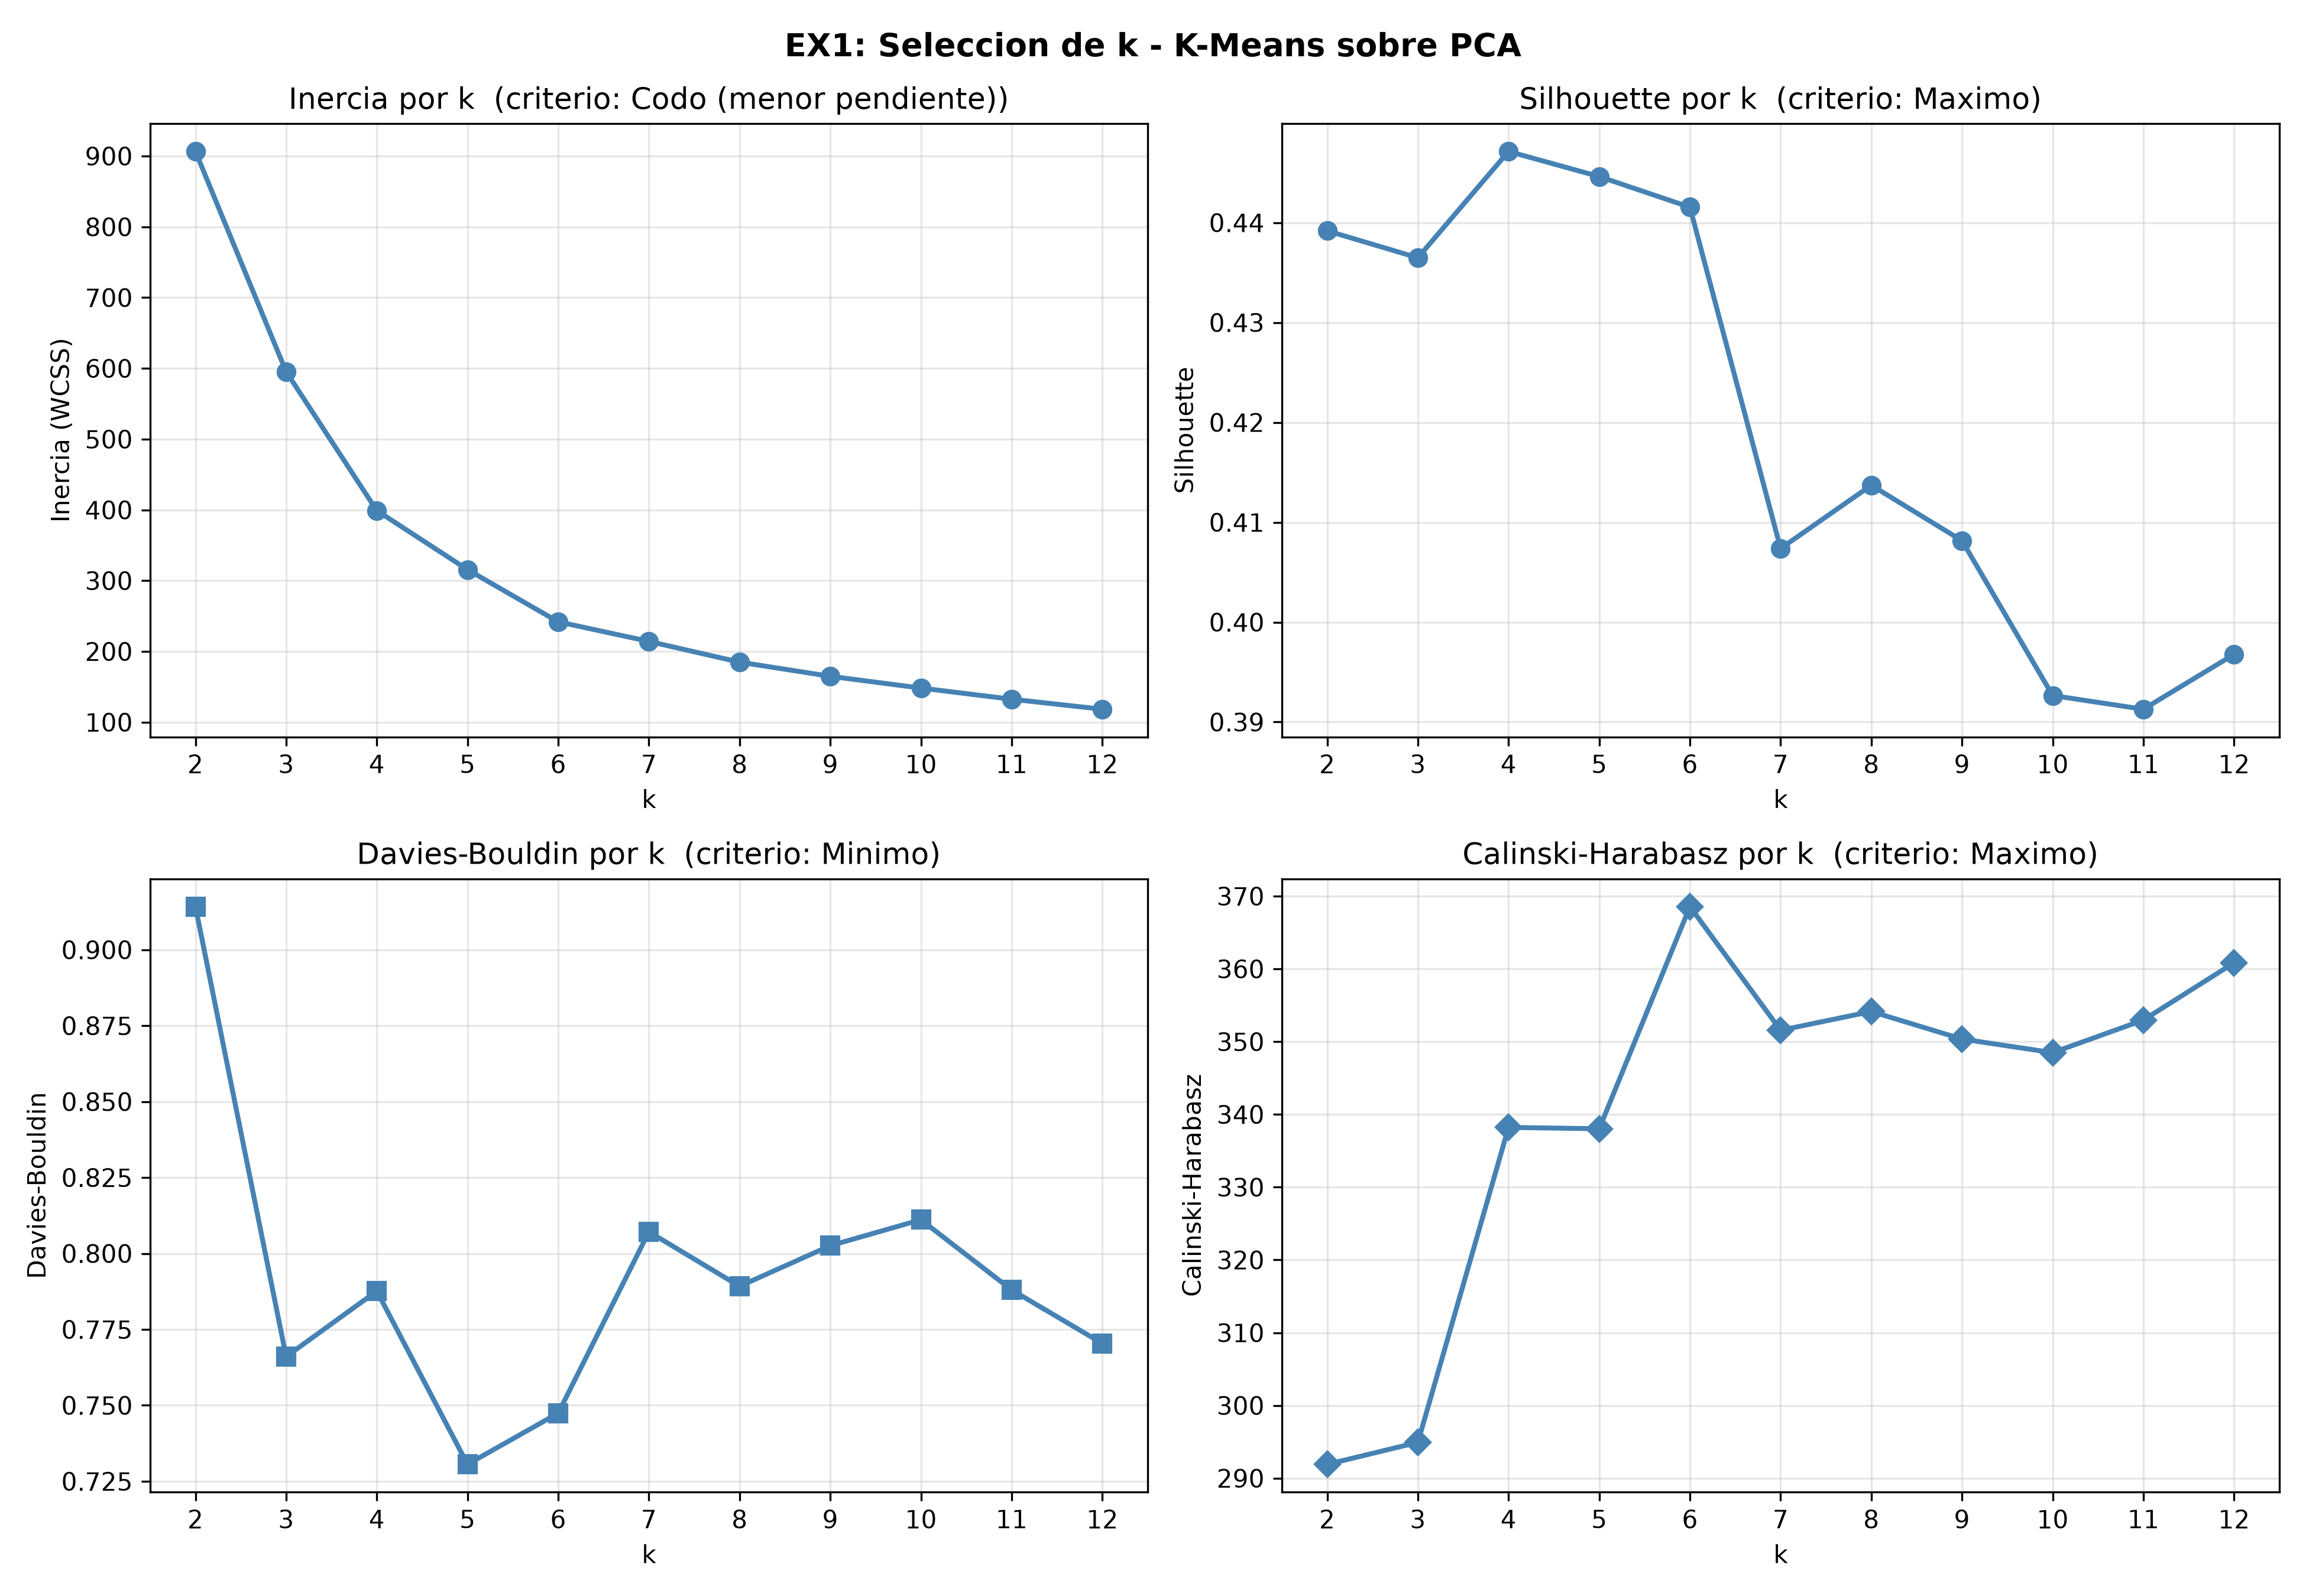
\includegraphics[width=\linewidth]{kmeans_codo_pca.png}
    \caption{EX1: selección de $k$ sobre PCA.}
    \label{fig:kmeans_codo_pca}
  \end{minipage}
  \hfill
  \begin{minipage}{0.48\linewidth}
    \centering
    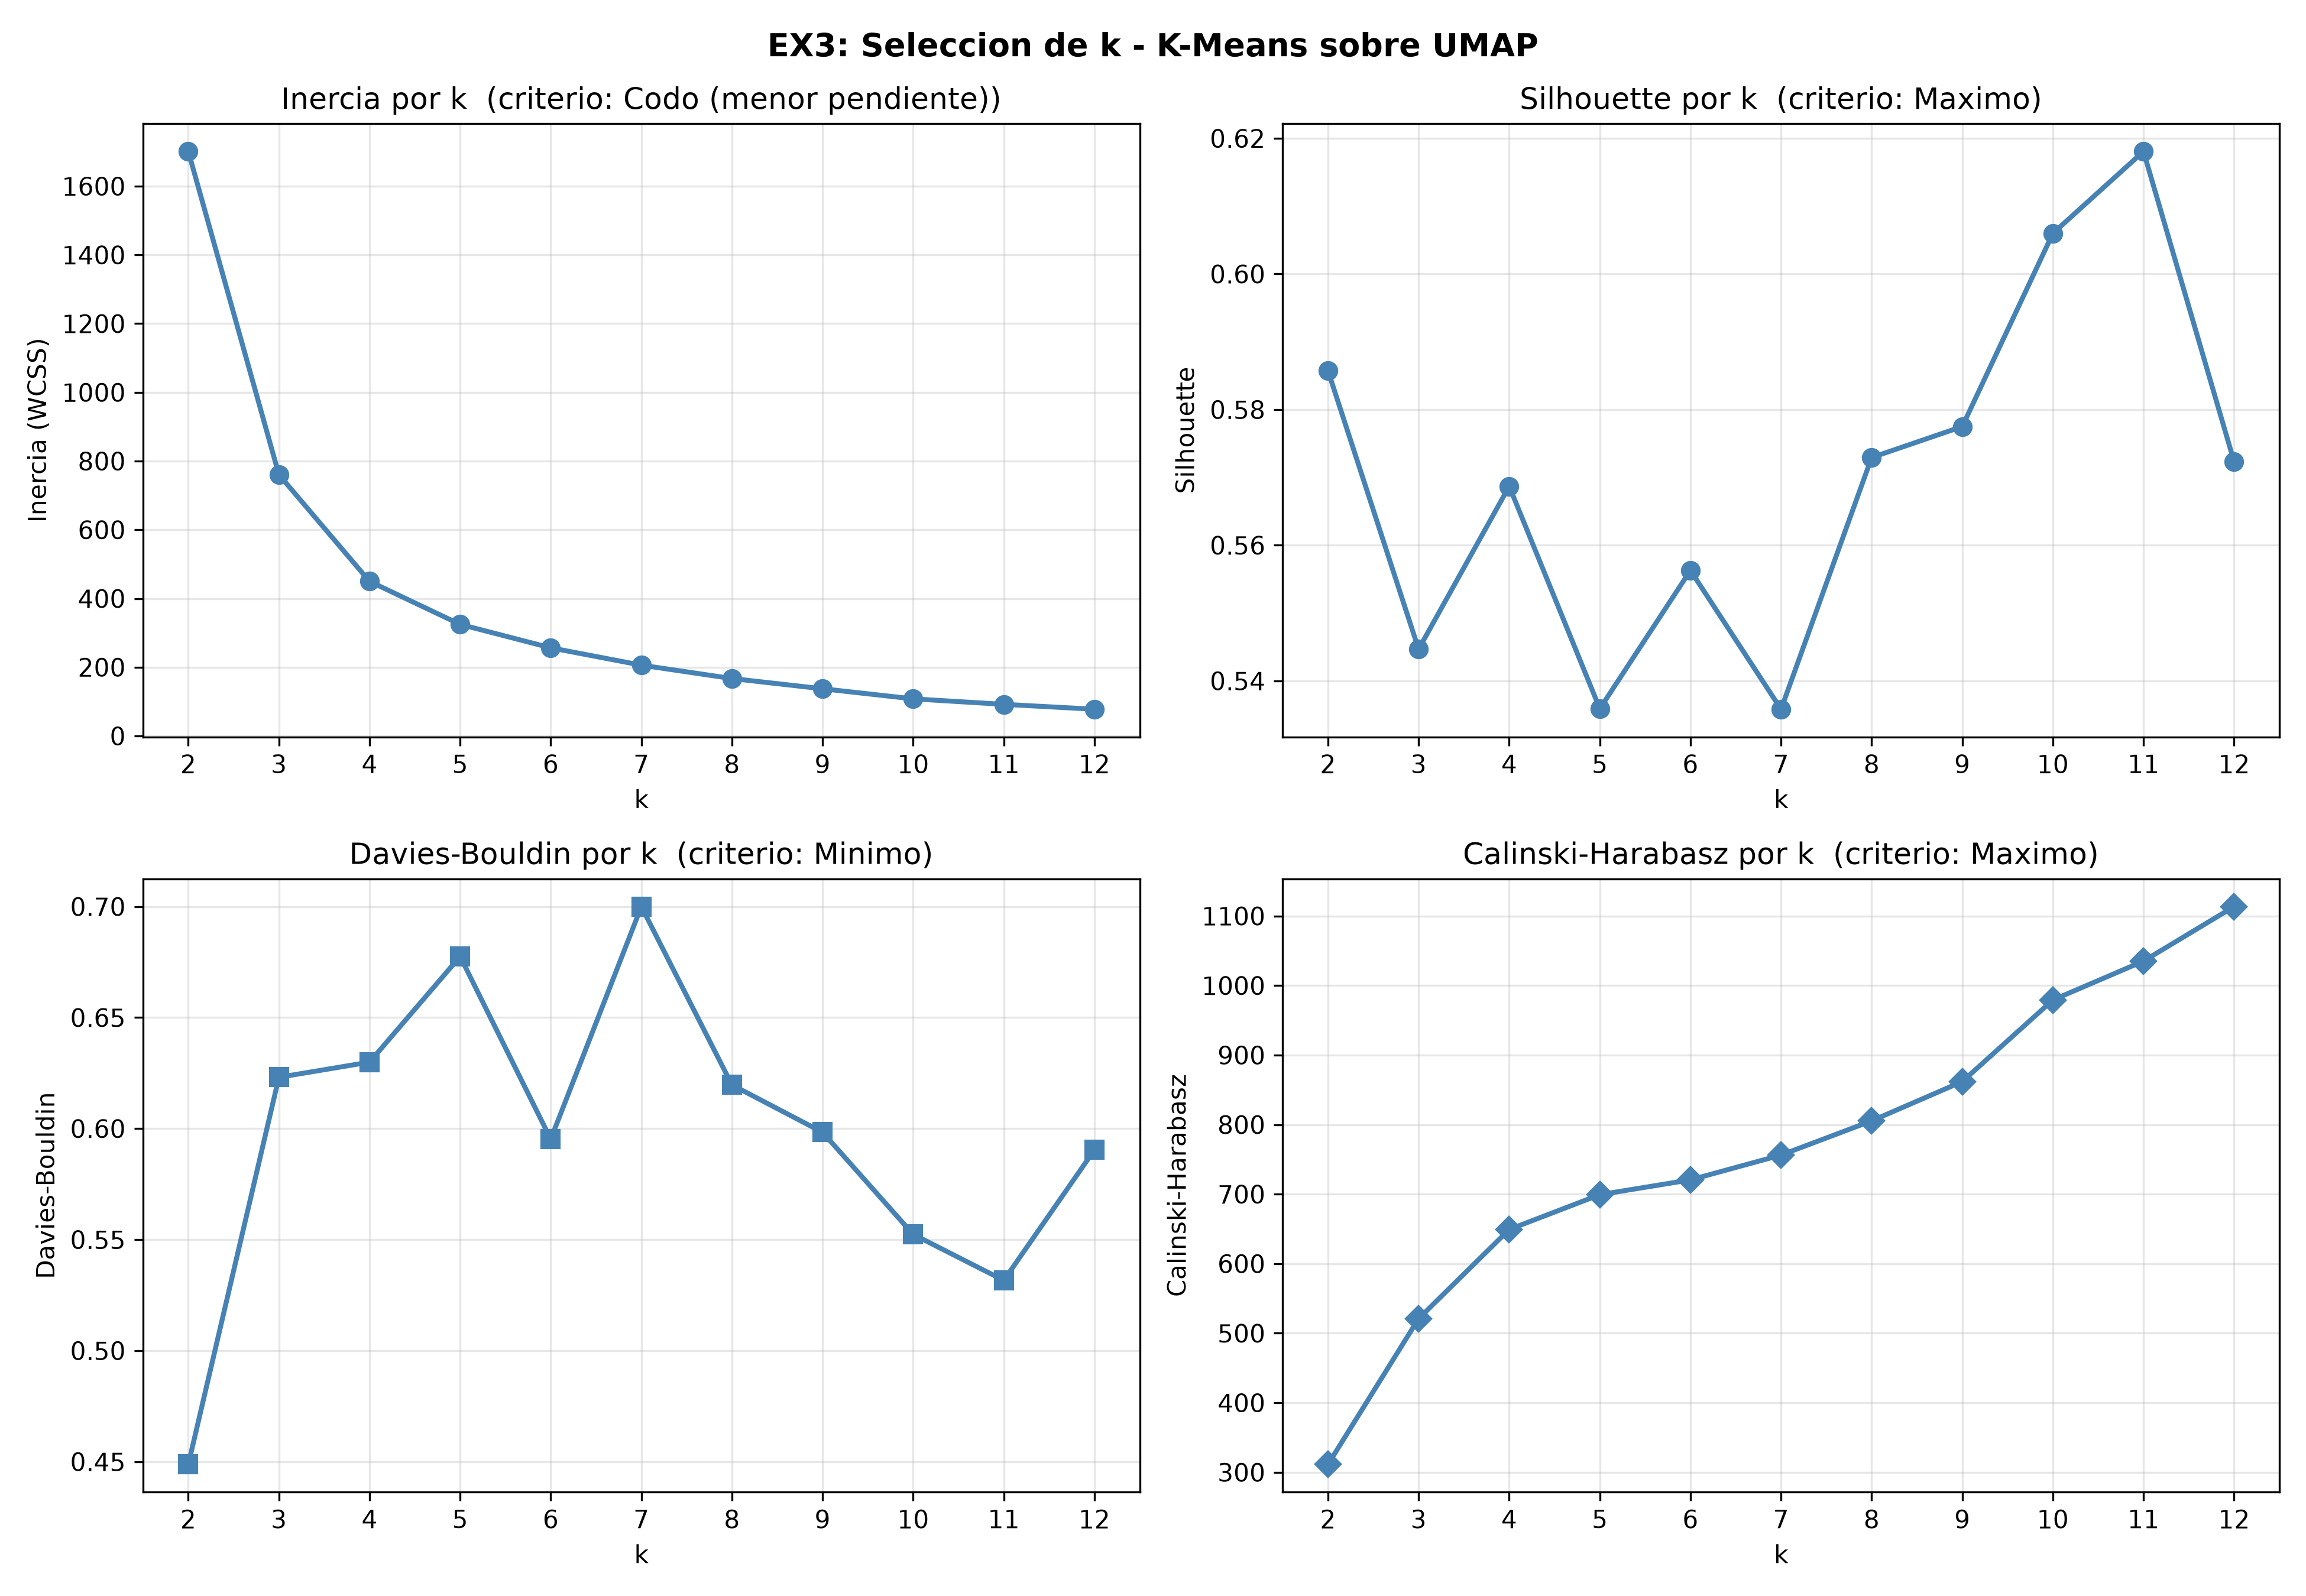
\includegraphics[width=\linewidth]{kmeans_codo_umap.png}
    \caption{EX3: selección de $k$ sobre UMAP.}
    \label{fig:kmeans_codo_umap}
  \end{minipage}
\end{figure}

\begin{figure}[H]
  \centering
  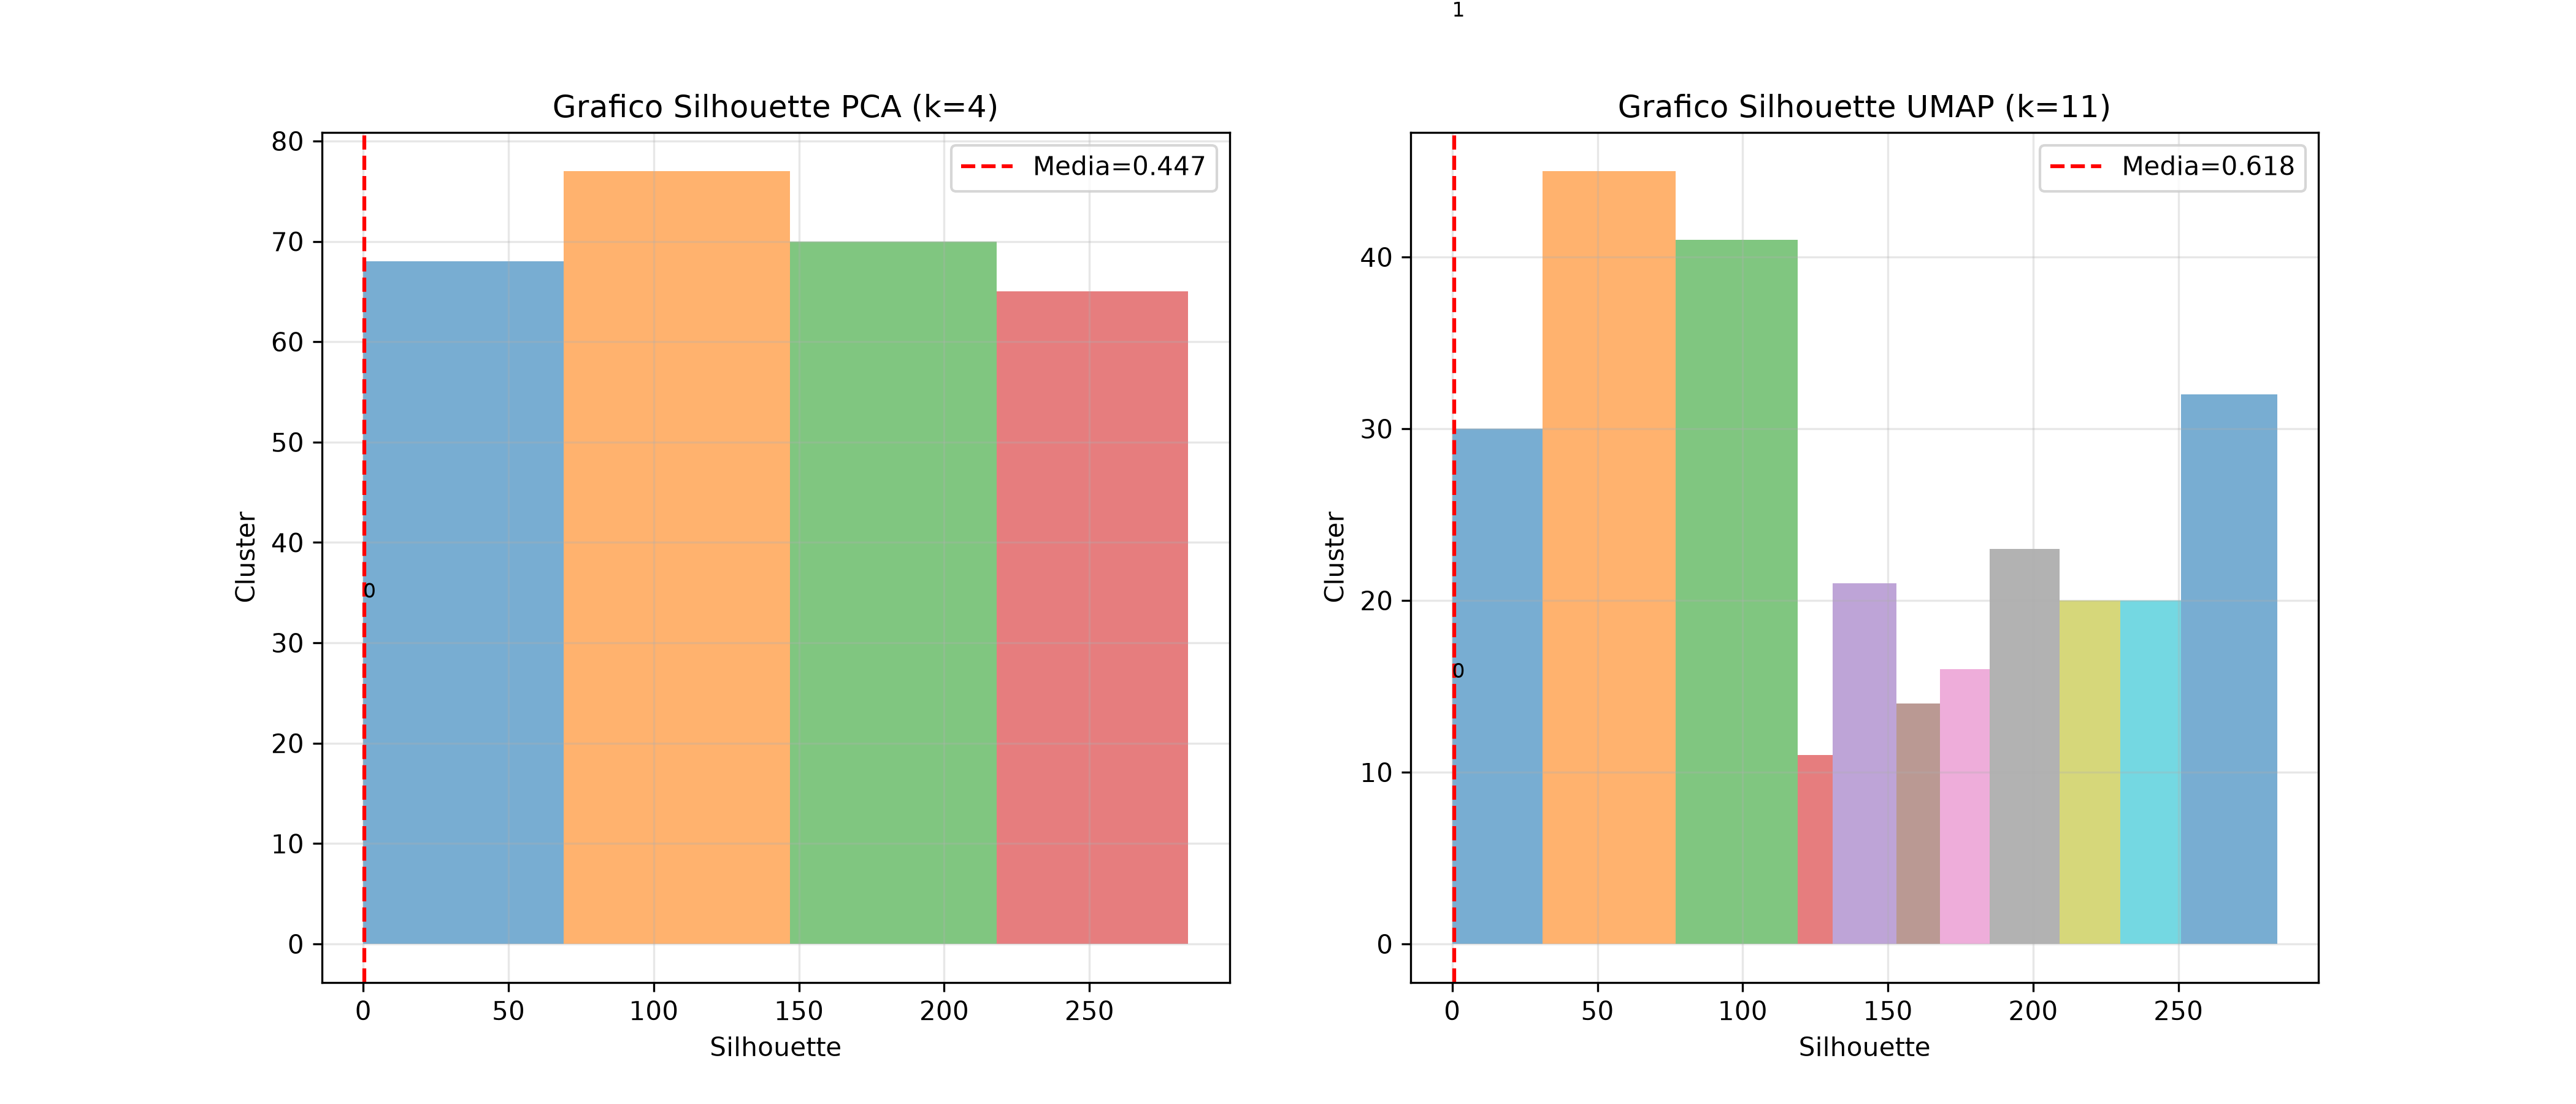
\includegraphics[width=0.9\linewidth]{kmeans_silhouette.png}
  \caption{Gráficos de silueta de los modelos óptimos EX1 ($k=4$) y EX3 ($k=11$).}
  \label{fig:kmeans_silhouette}
\end{figure}

\begin{figure}[H]
  \centering
  \begin{minipage}{0.48\linewidth}
    \centering
    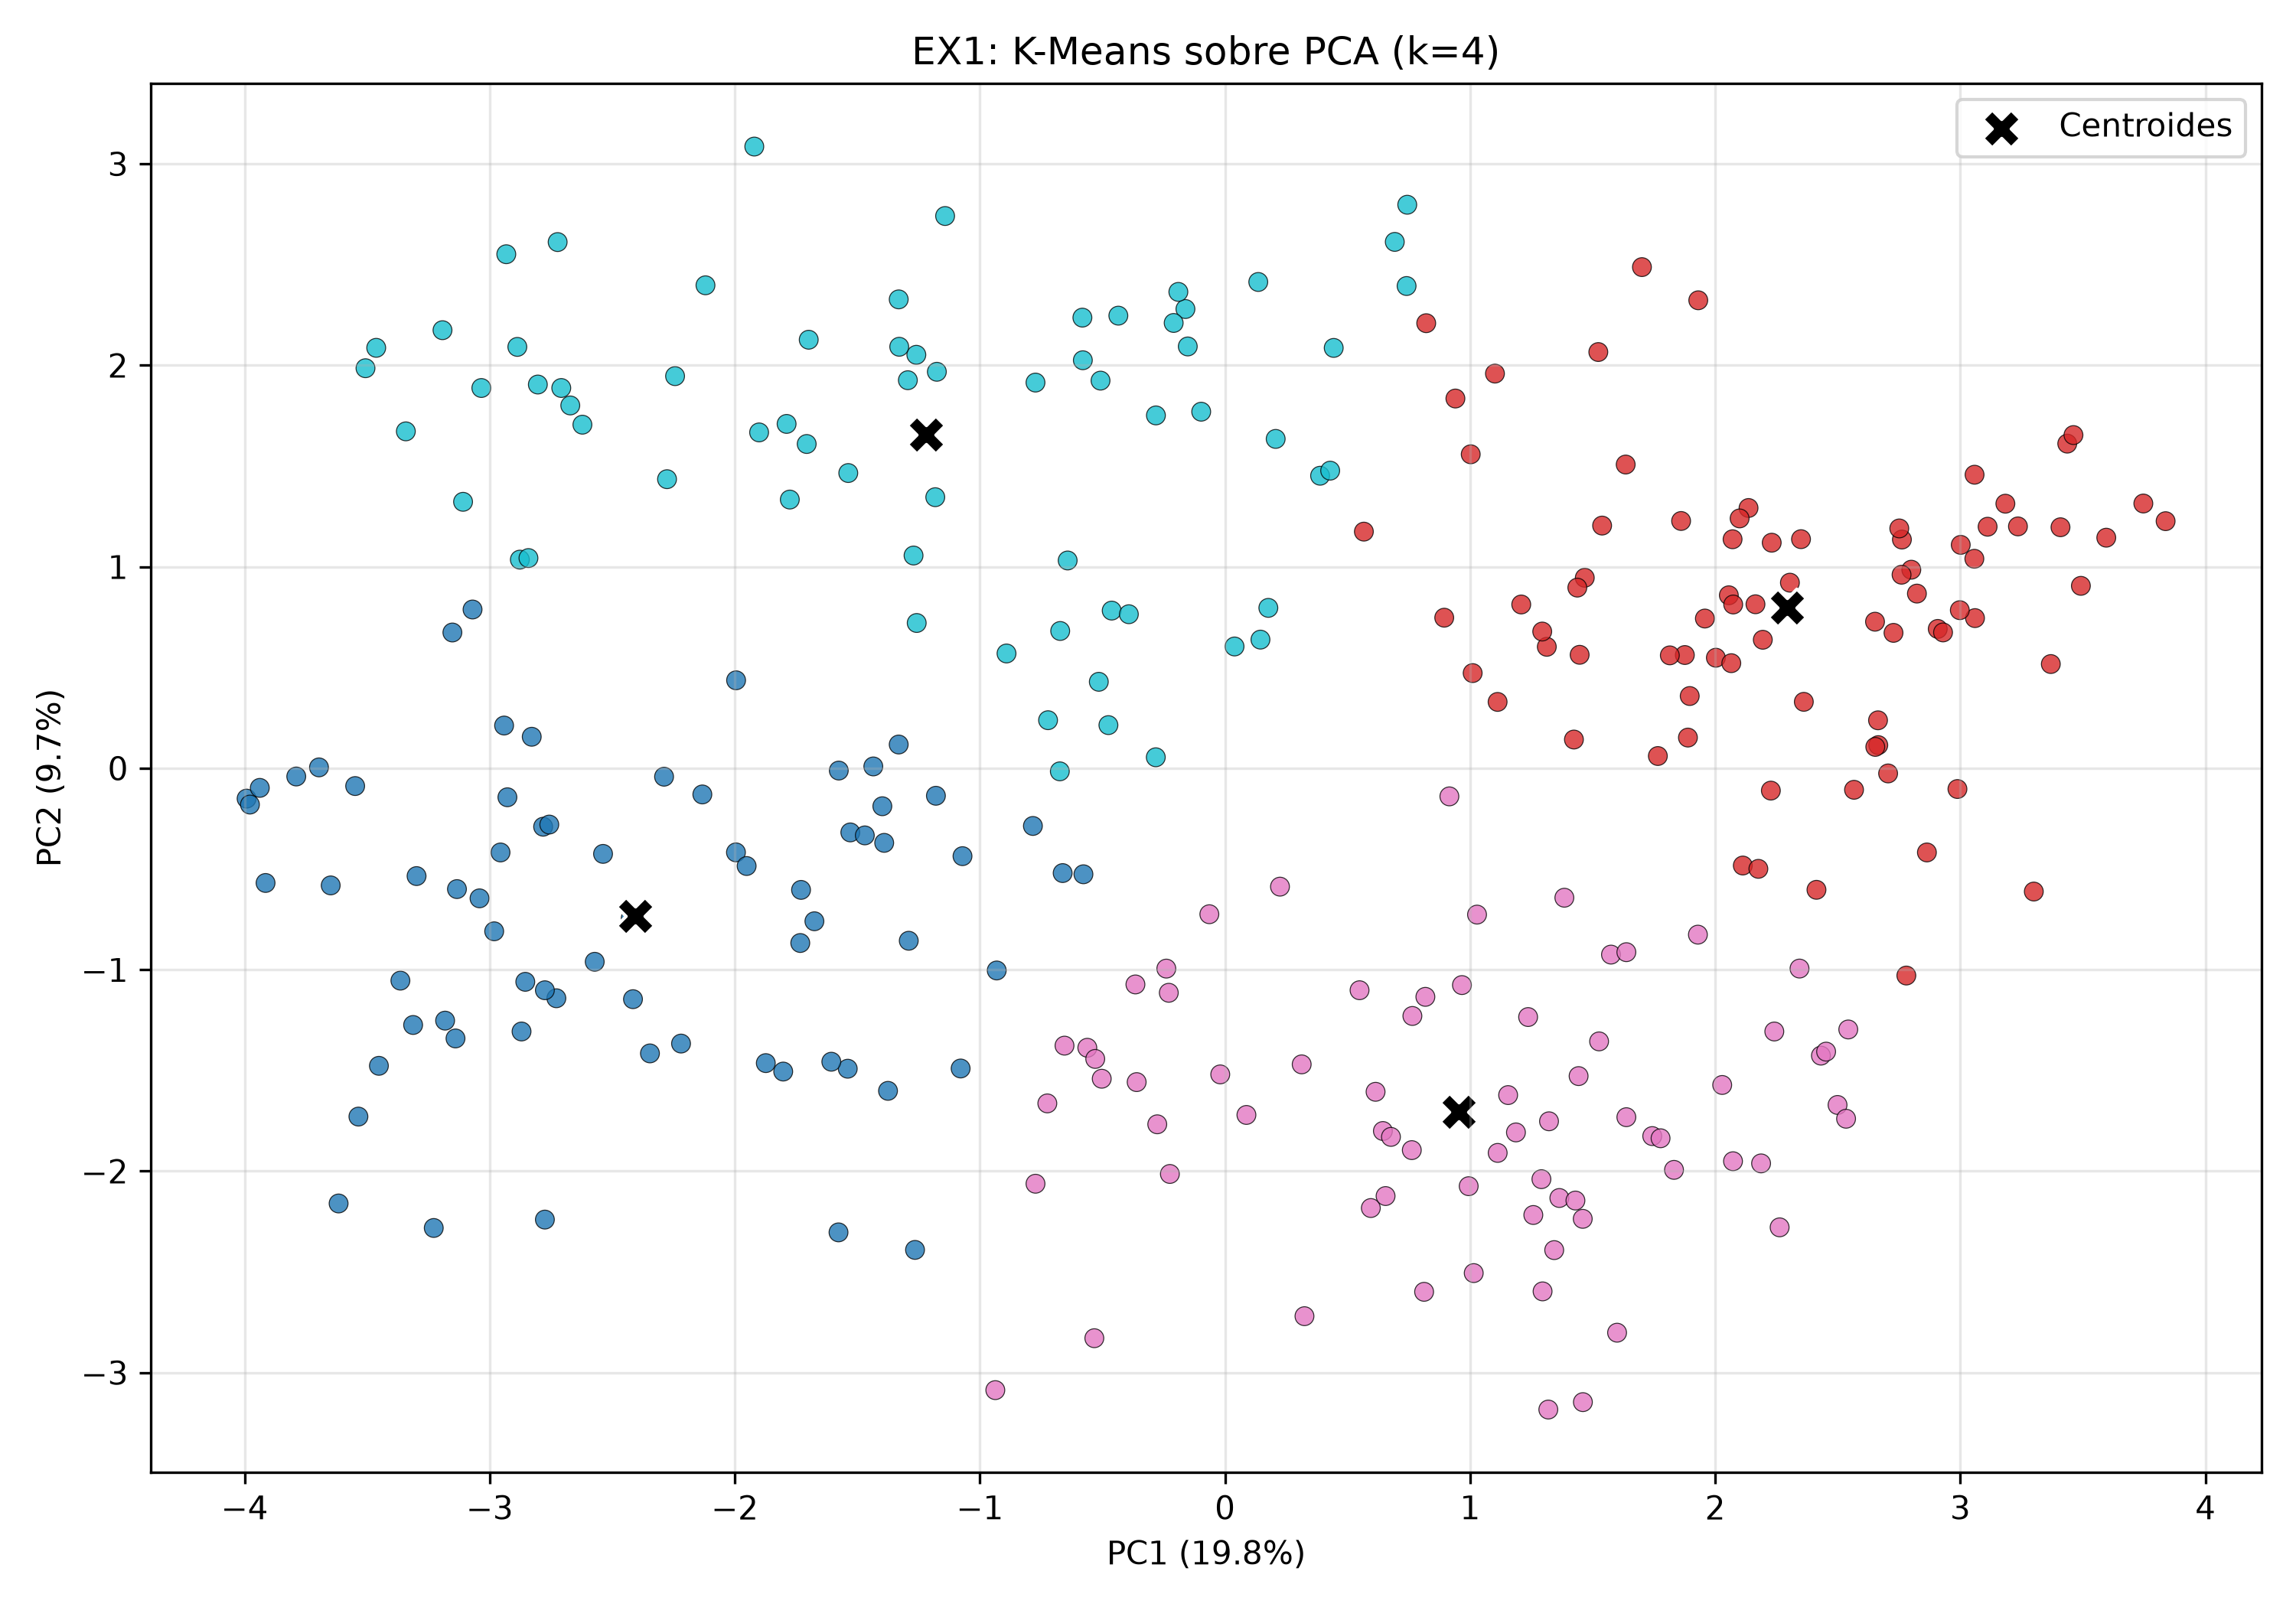
\includegraphics[width=\linewidth]{kmeans_pca.png}
    \caption{EX1: K-Means sobre PCA ($k=4$) con centroides.}
    \label{fig:kmeans_pca}
  \end{minipage}
  \hfill
  \begin{minipage}{0.48\linewidth}
    \centering
    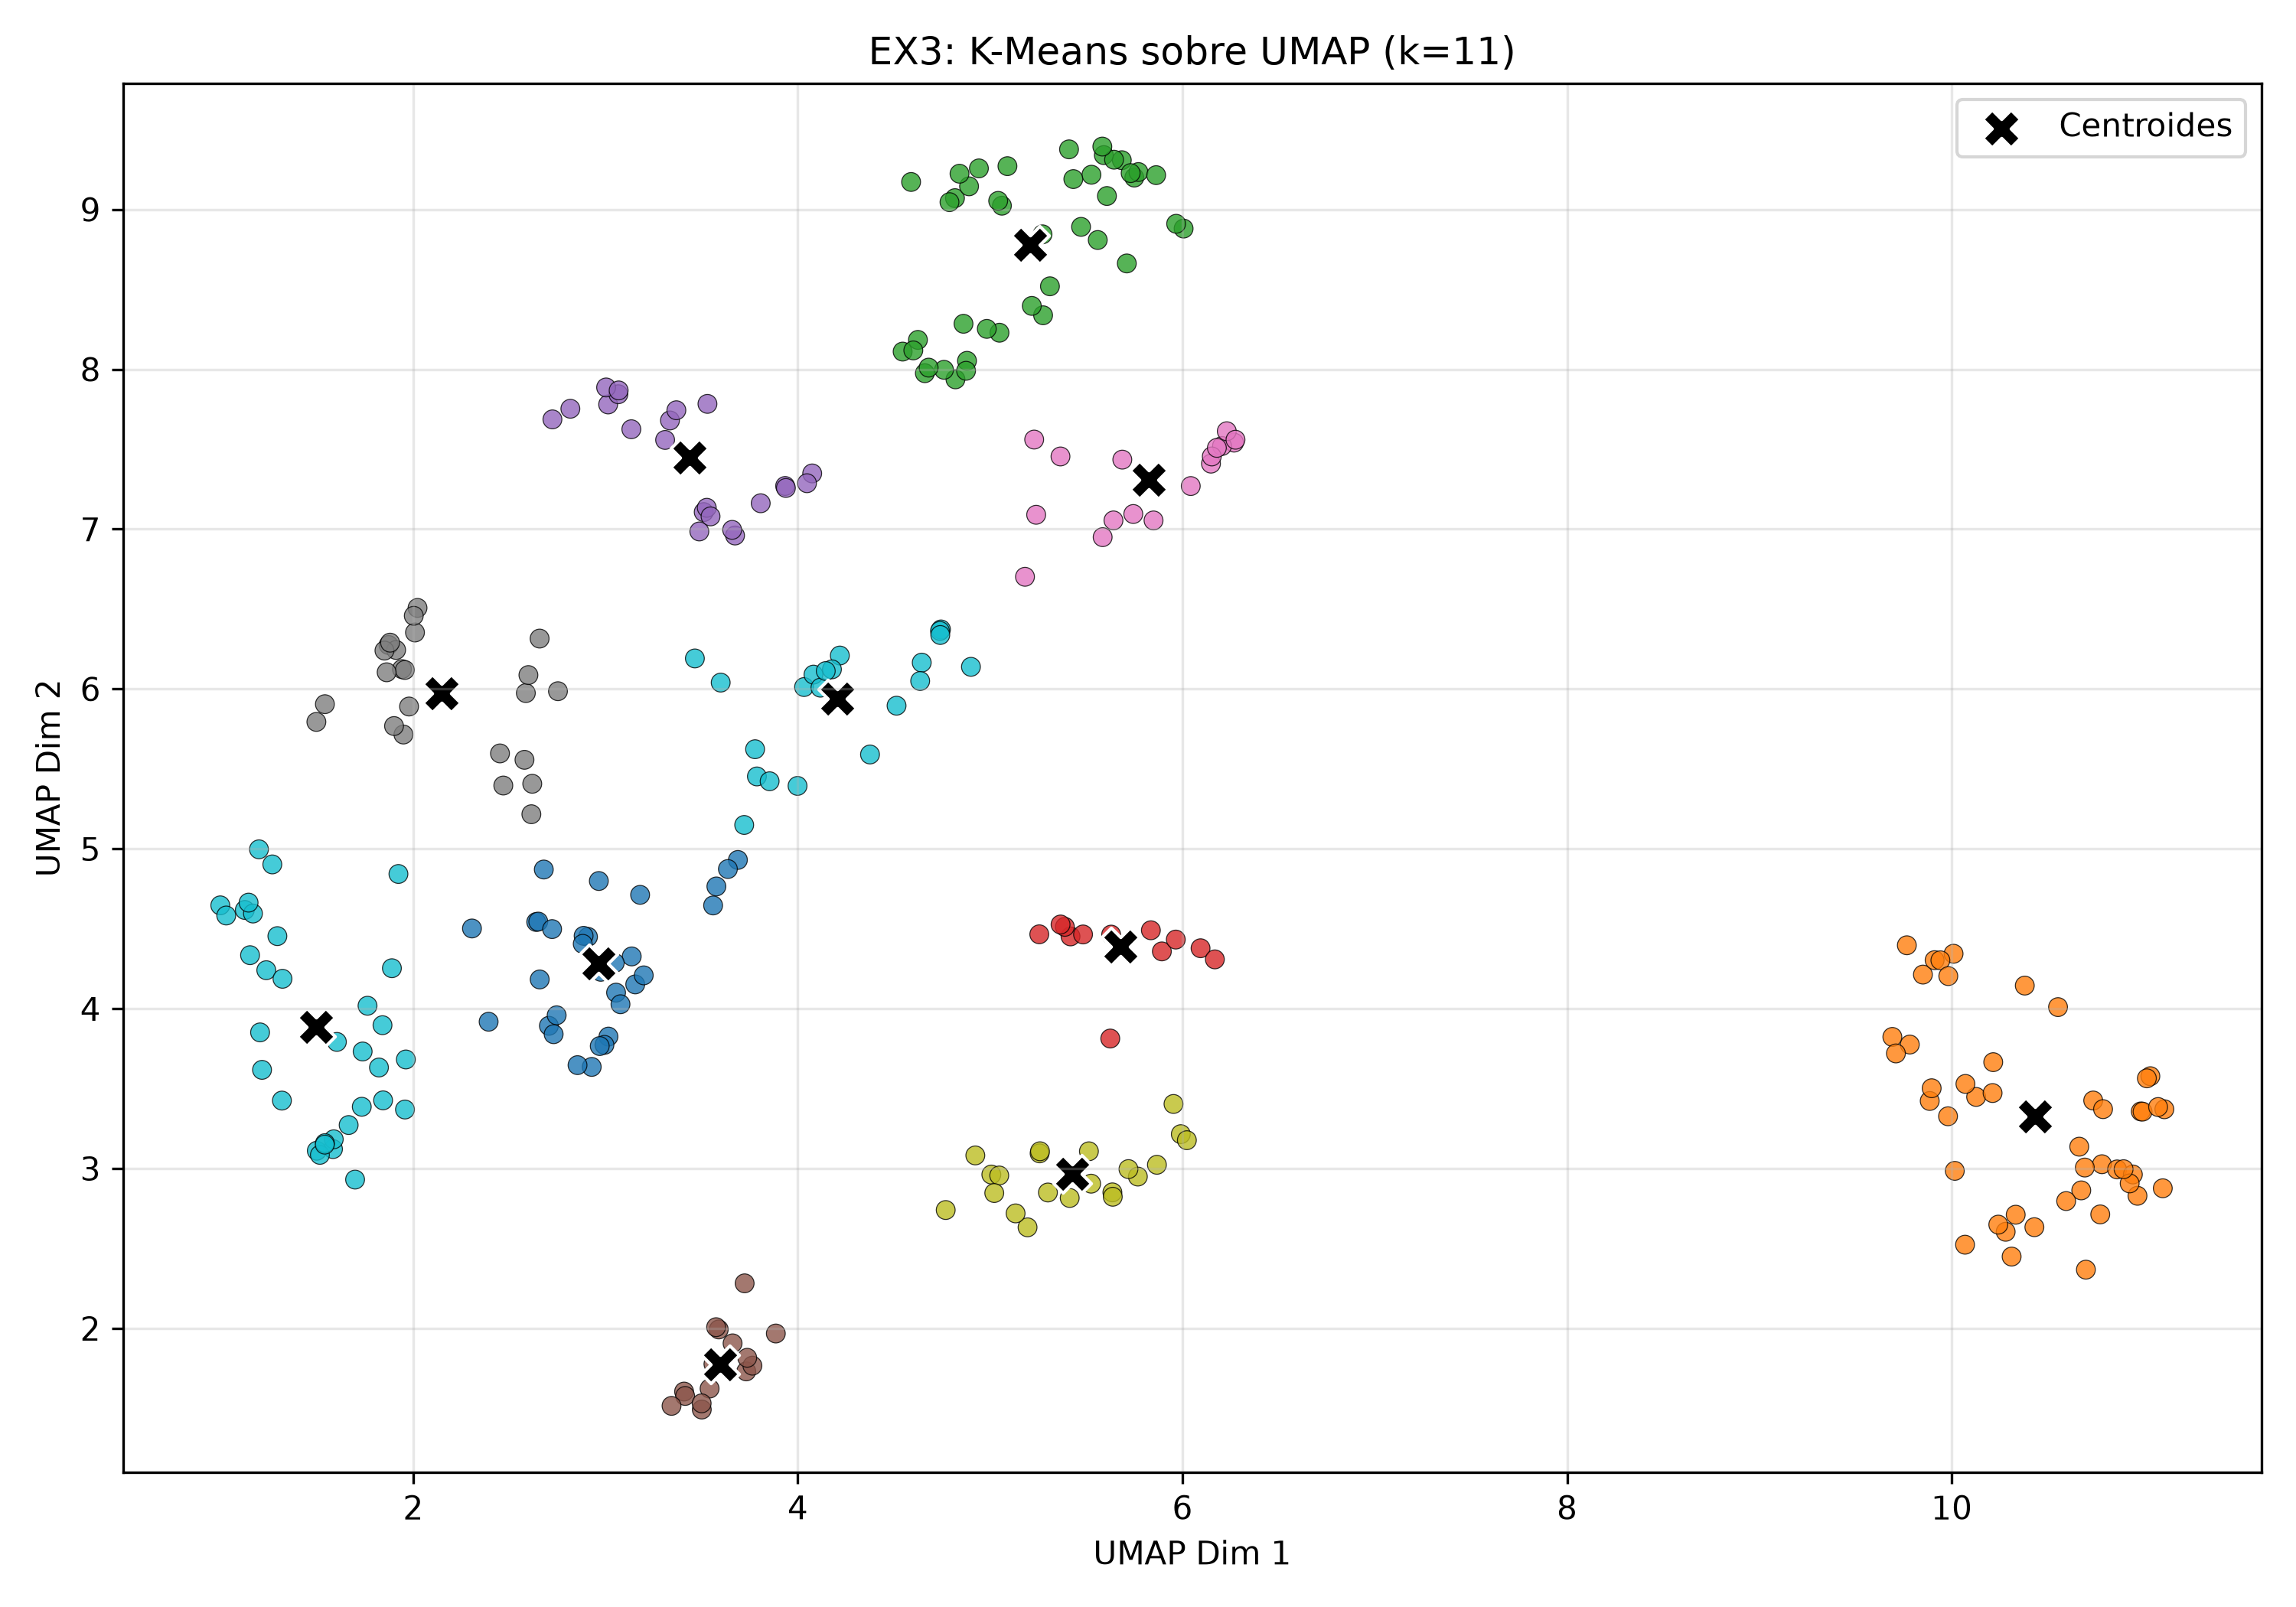
\includegraphics[width=\linewidth]{kmeans_umap.png}
    \caption{EX3: K-Means sobre UMAP ($k=11$) con centroides.}
    \label{fig:kmeans_umap}
  \end{minipage}
\end{figure}

\begin{figure}[H]
  \centering
  \begin{minipage}{0.48\linewidth}
    \centering
    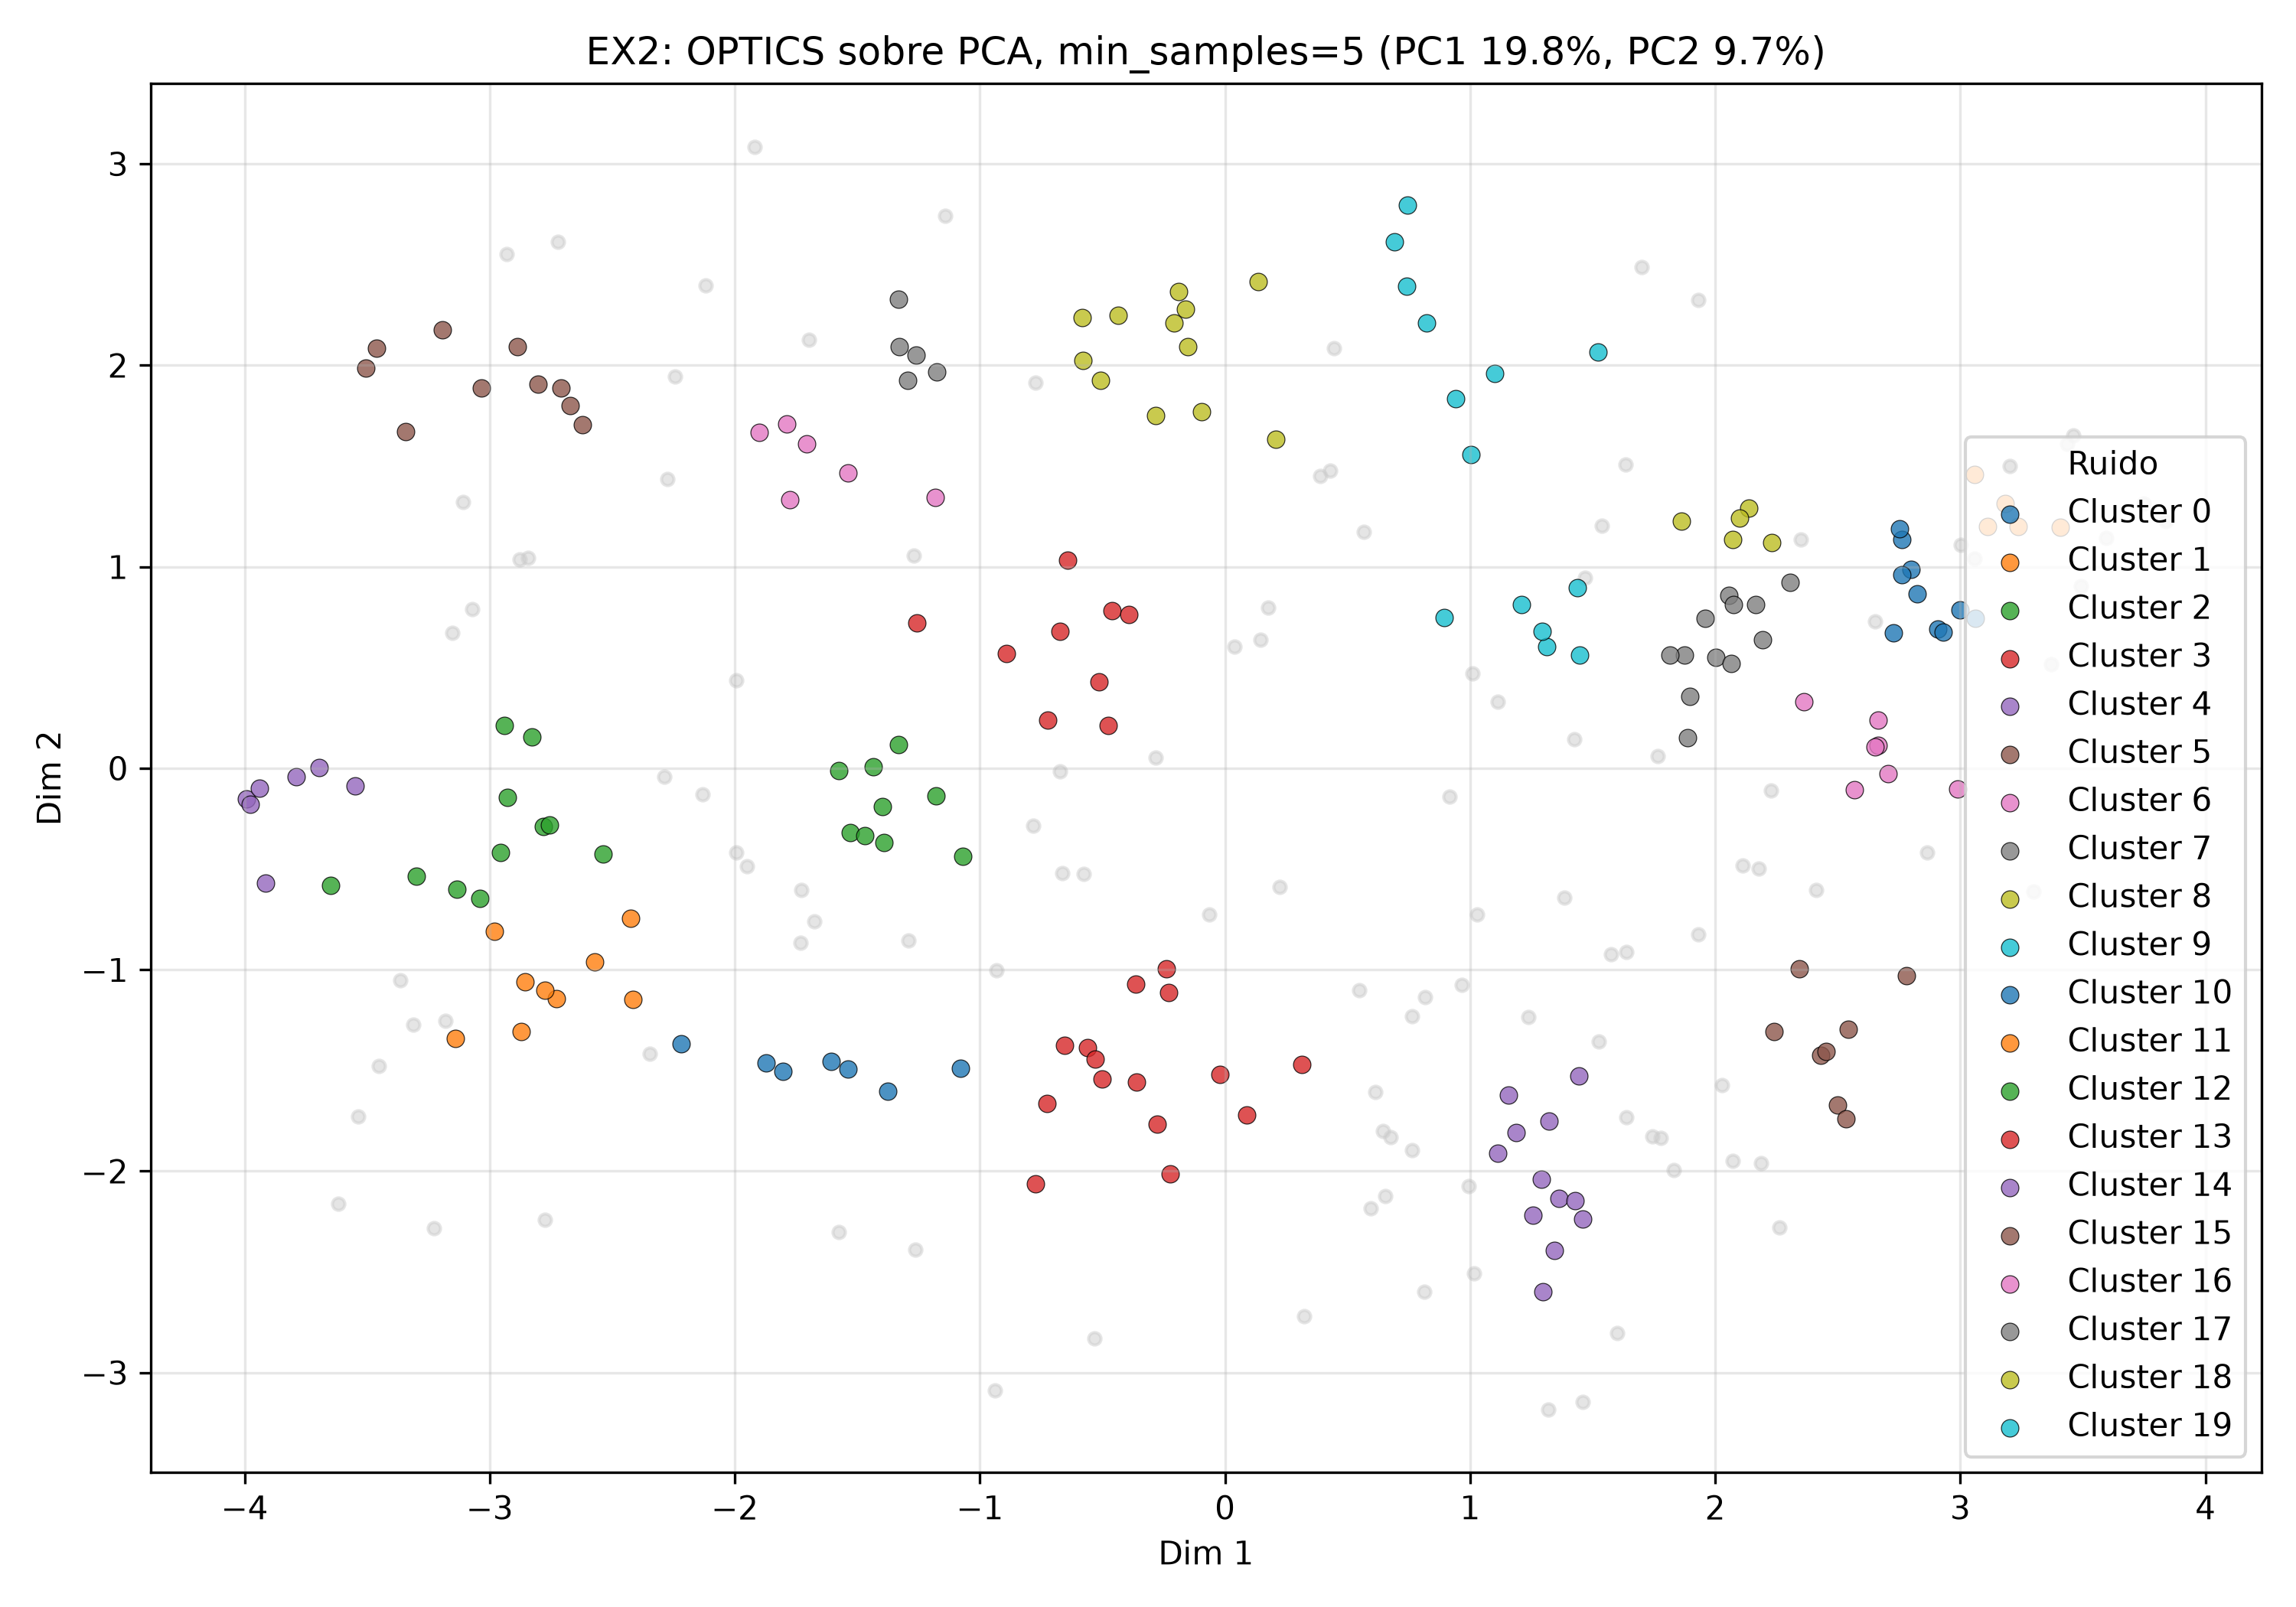
\includegraphics[width=\linewidth]{optics_pca.png}
    \caption{EX2: OPTICS sobre PCA (ms=5).}
    \label{fig:optics_pca}
  \end{minipage}
  \hfill
  \begin{minipage}{0.48\linewidth}
    \centering
    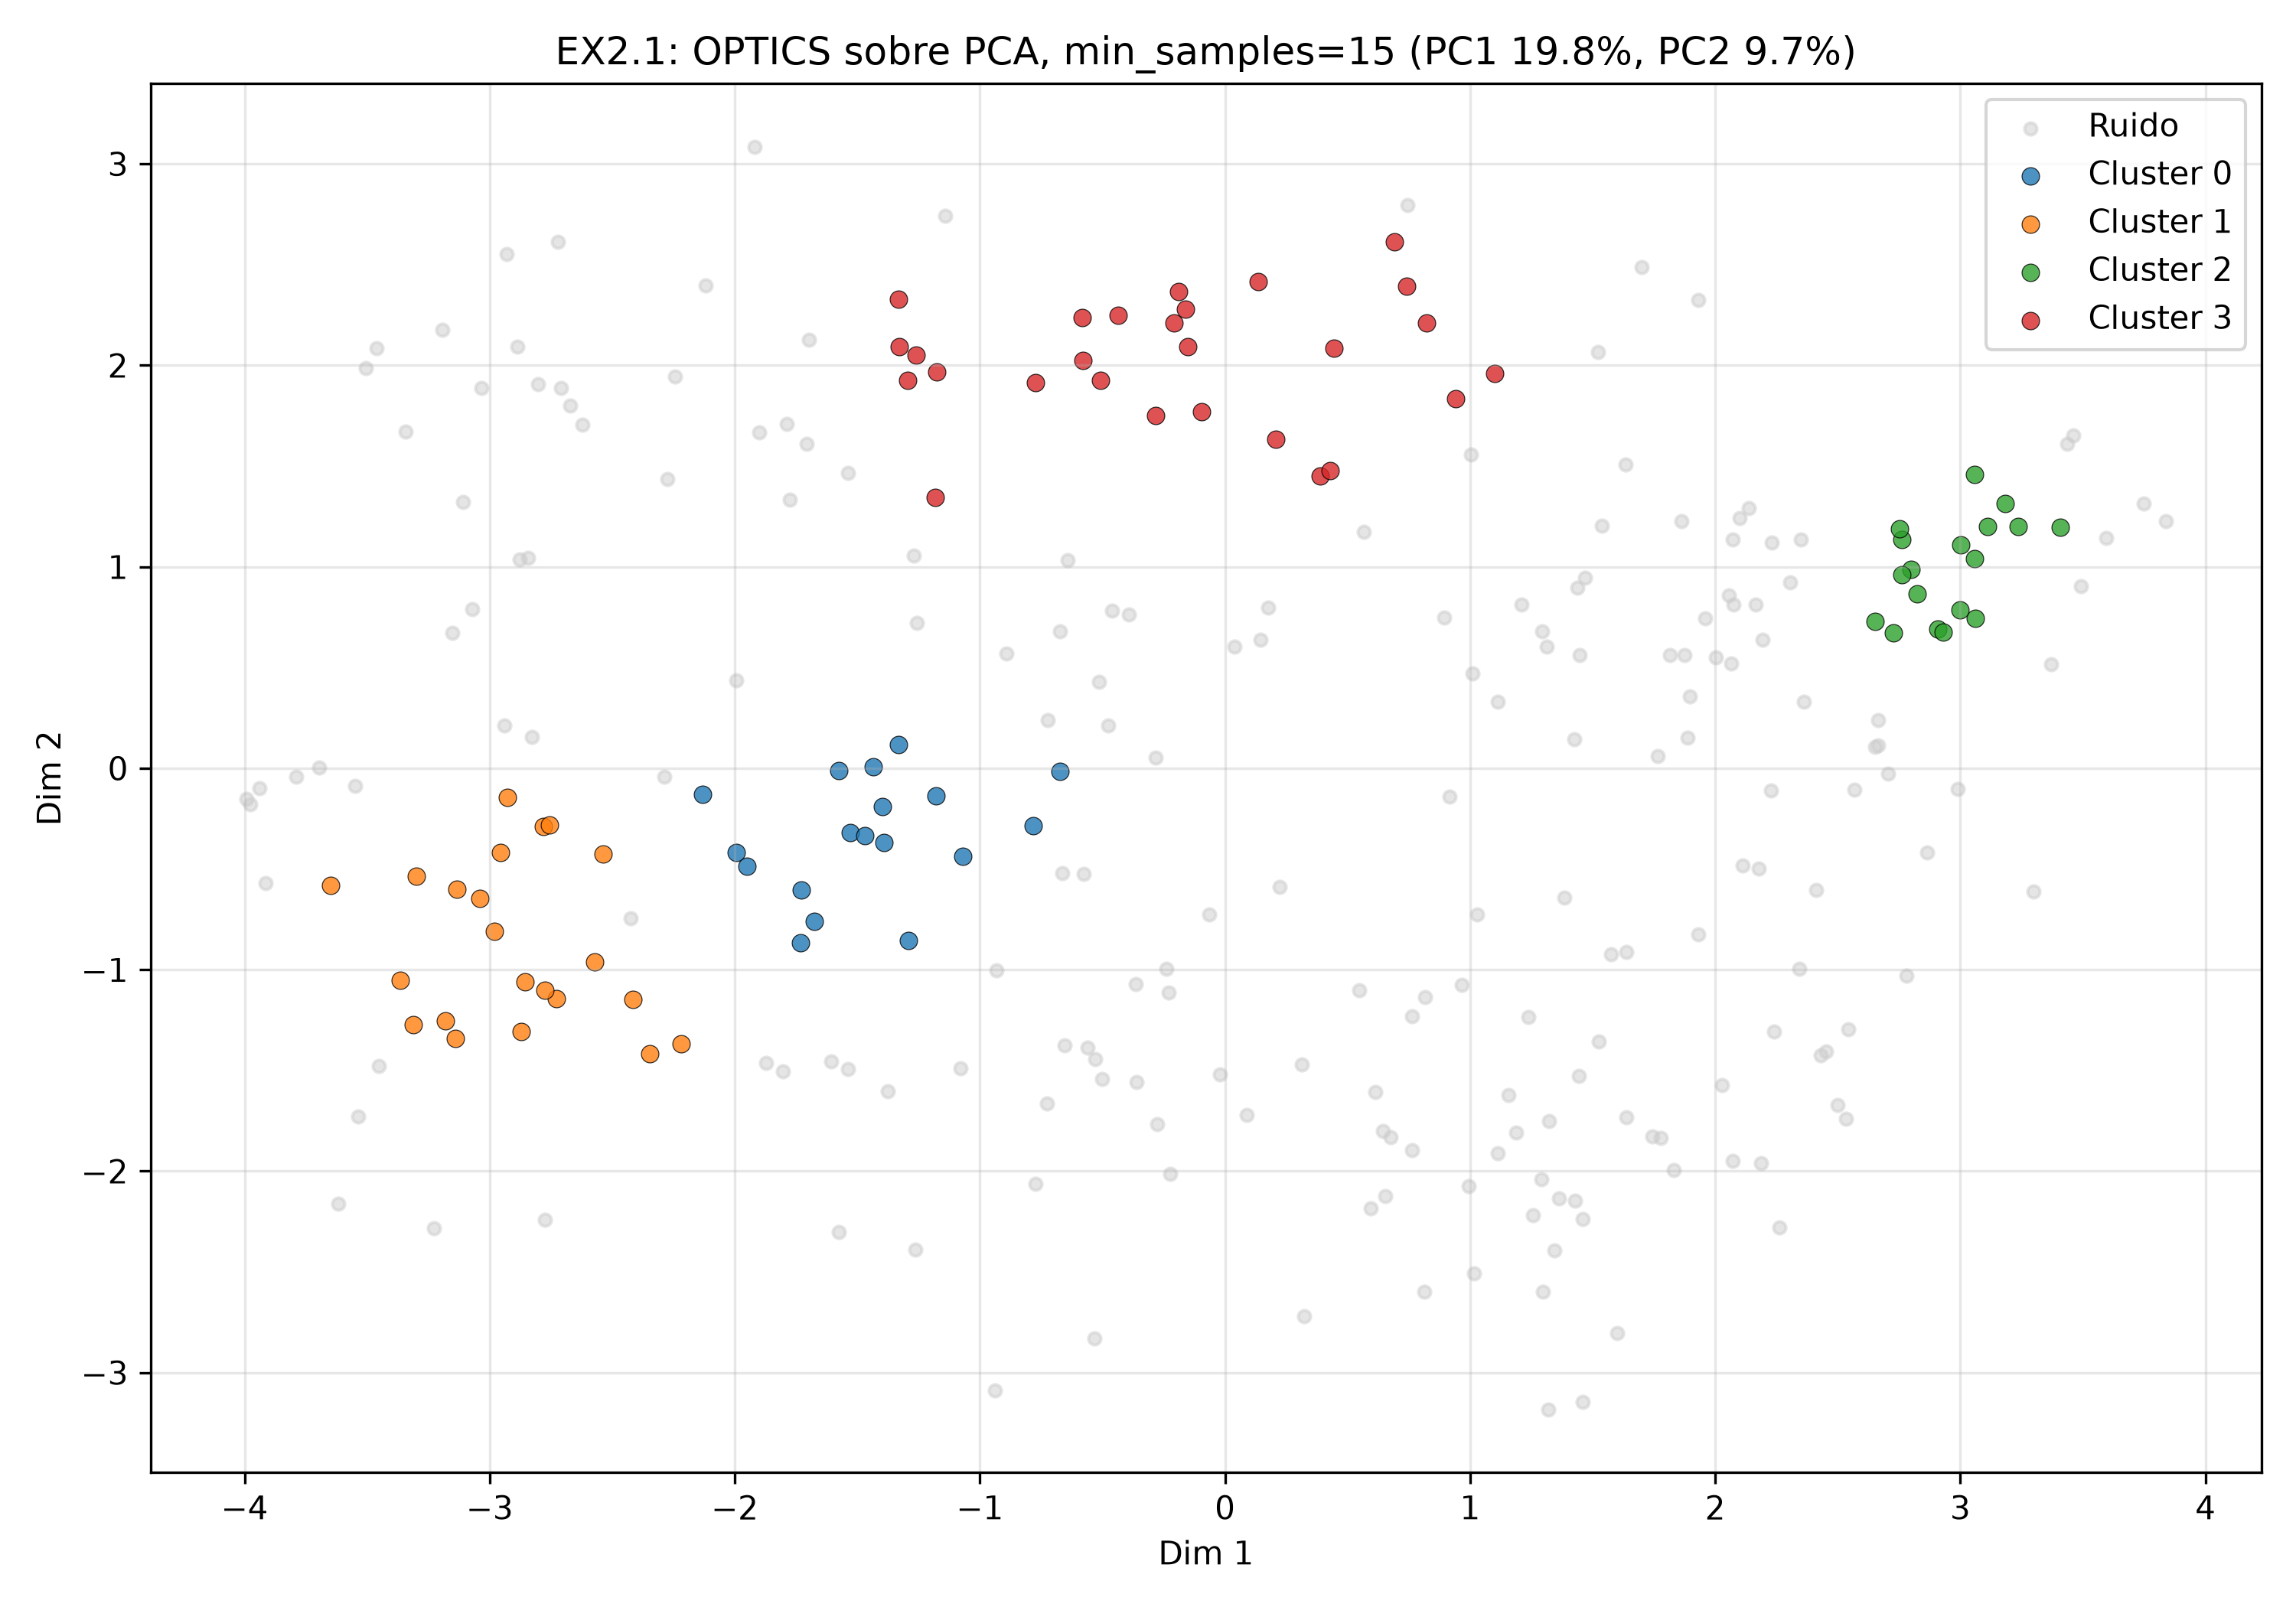
\includegraphics[width=\linewidth]{optics_pca_ms15.png}
    \caption{EX2.1: OPTICS sobre PCA (ms=15).}
    \label{fig:optics_pca_ms15}
  \end{minipage}
\end{figure}

\begin{figure}[H]
  \centering
  \begin{minipage}{0.48\linewidth}
    \centering
    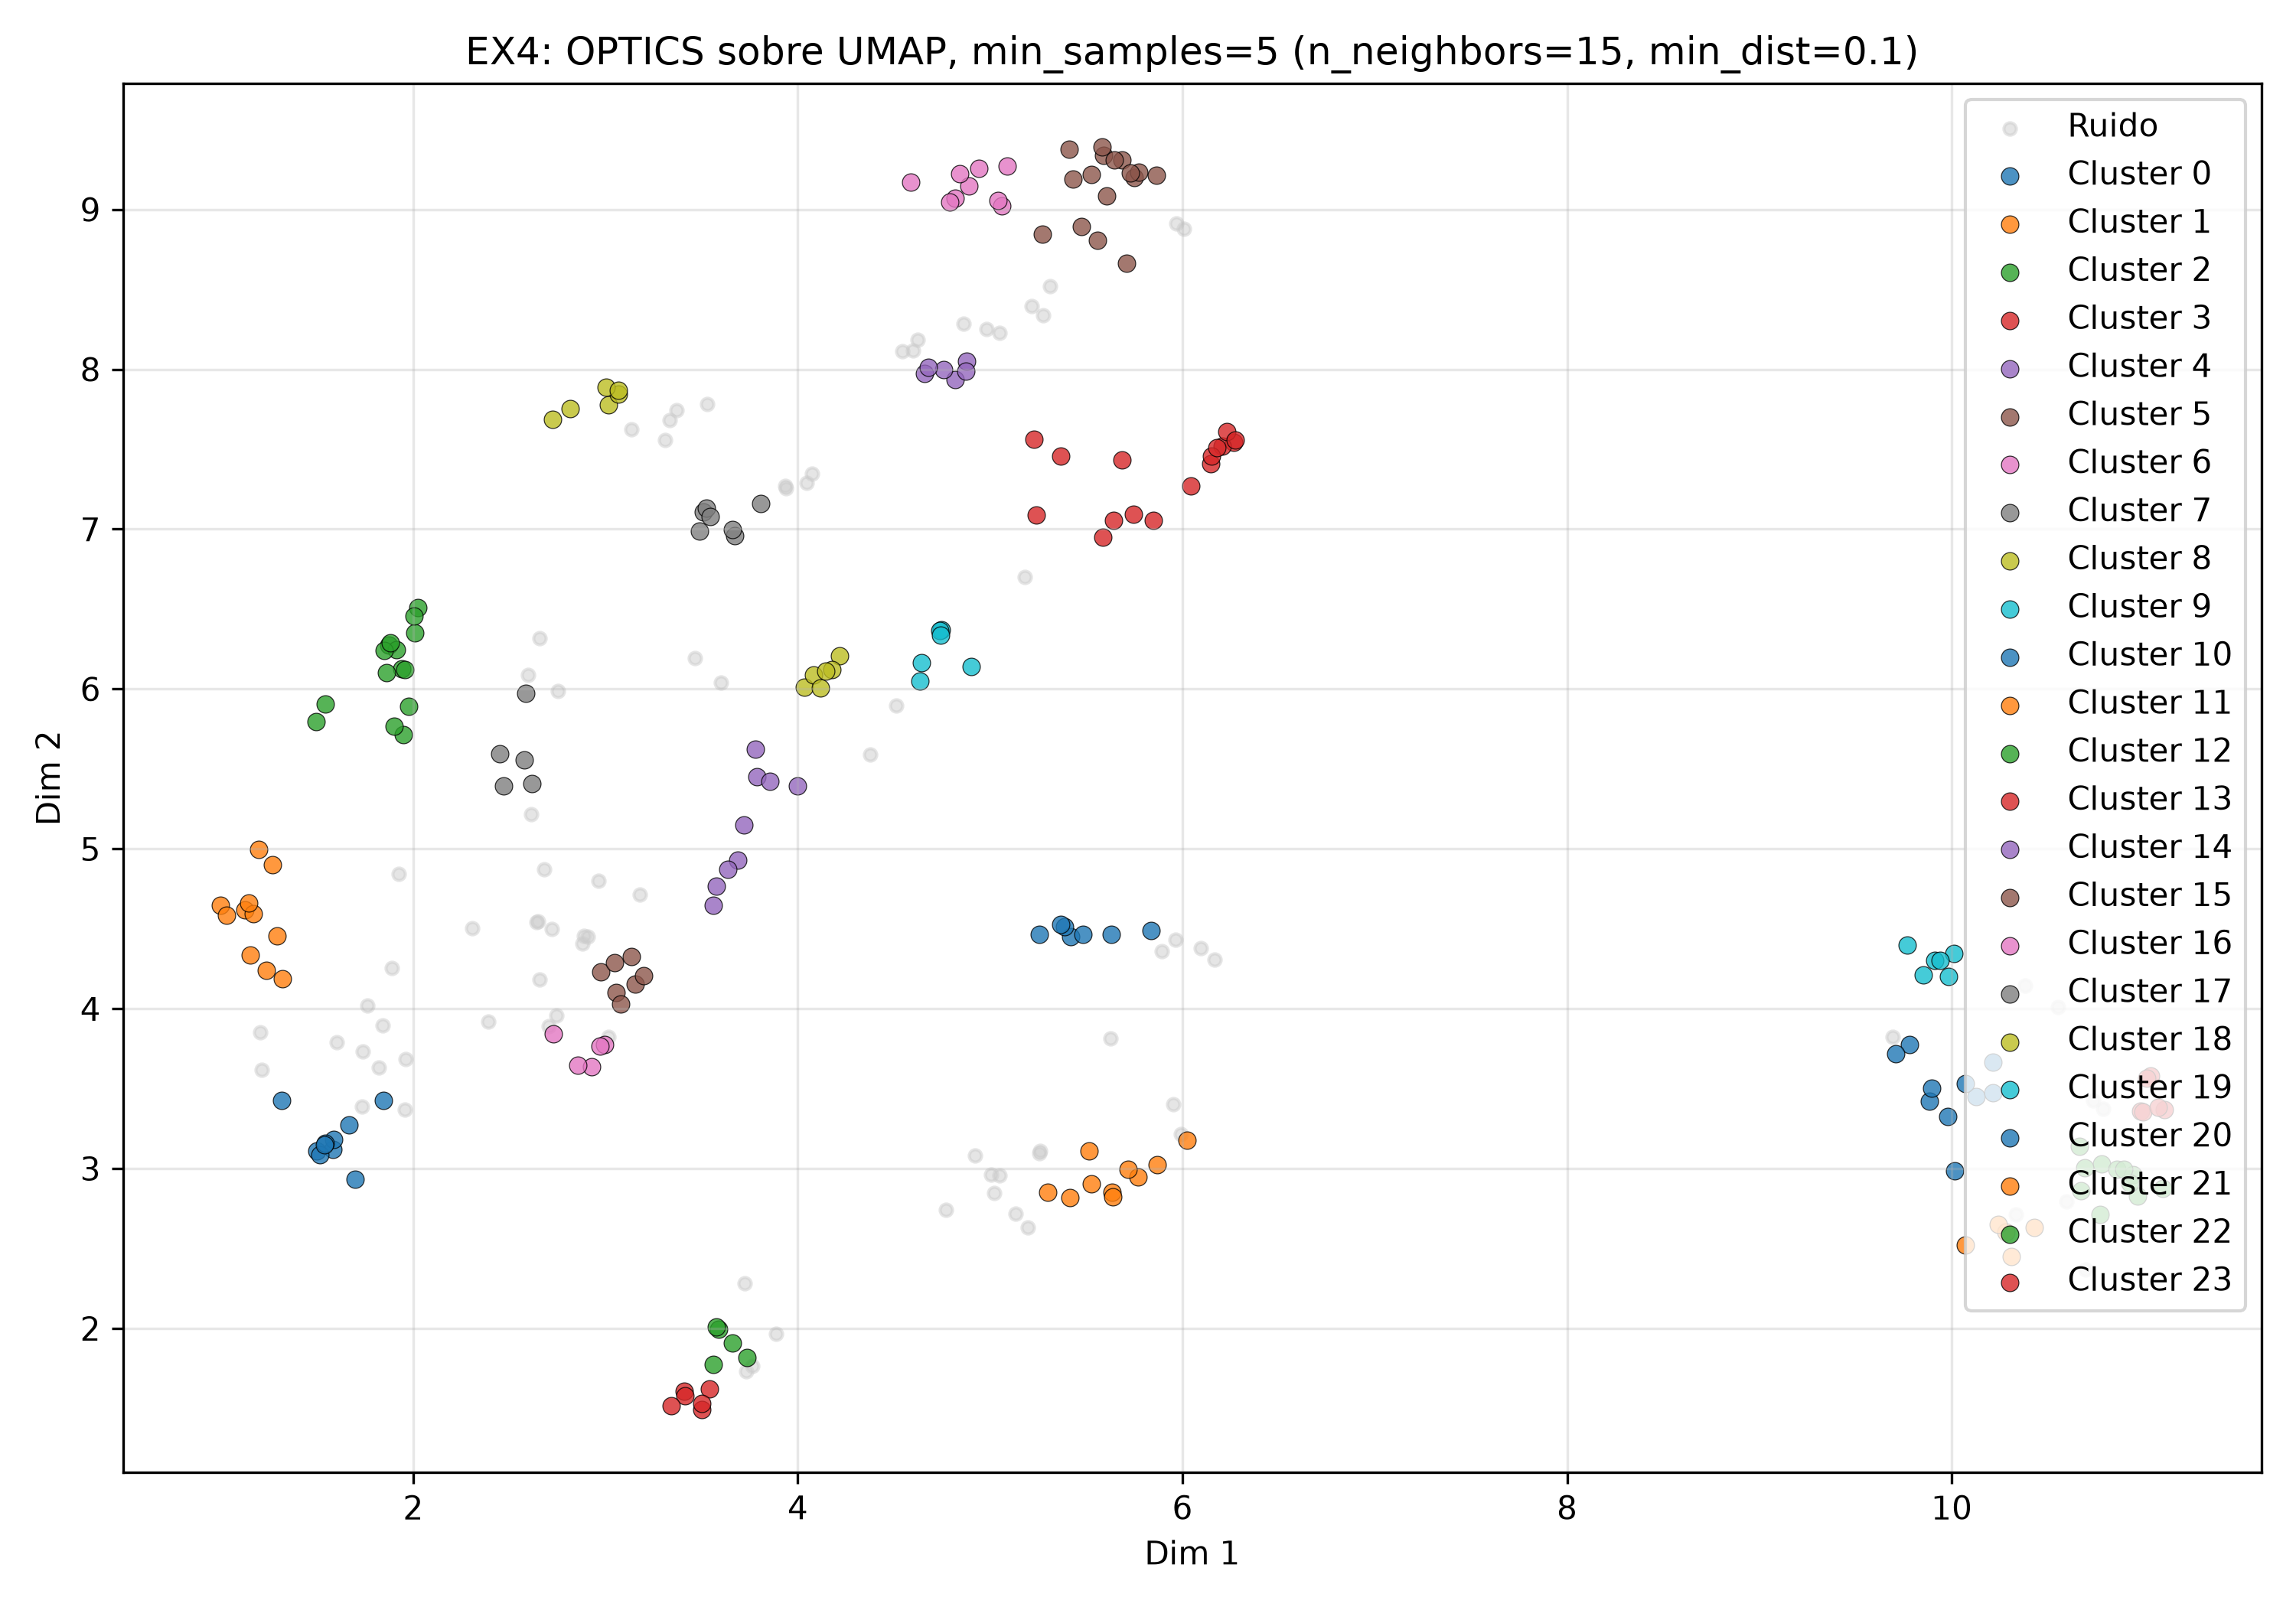
\includegraphics[width=\linewidth]{optics_umap.png}
    \caption{EX4: OPTICS sobre UMAP (ms=5).}
    \label{fig:optics_umap}
  \end{minipage}
  \hfill
  \begin{minipage}{0.48\linewidth}
    \centering
    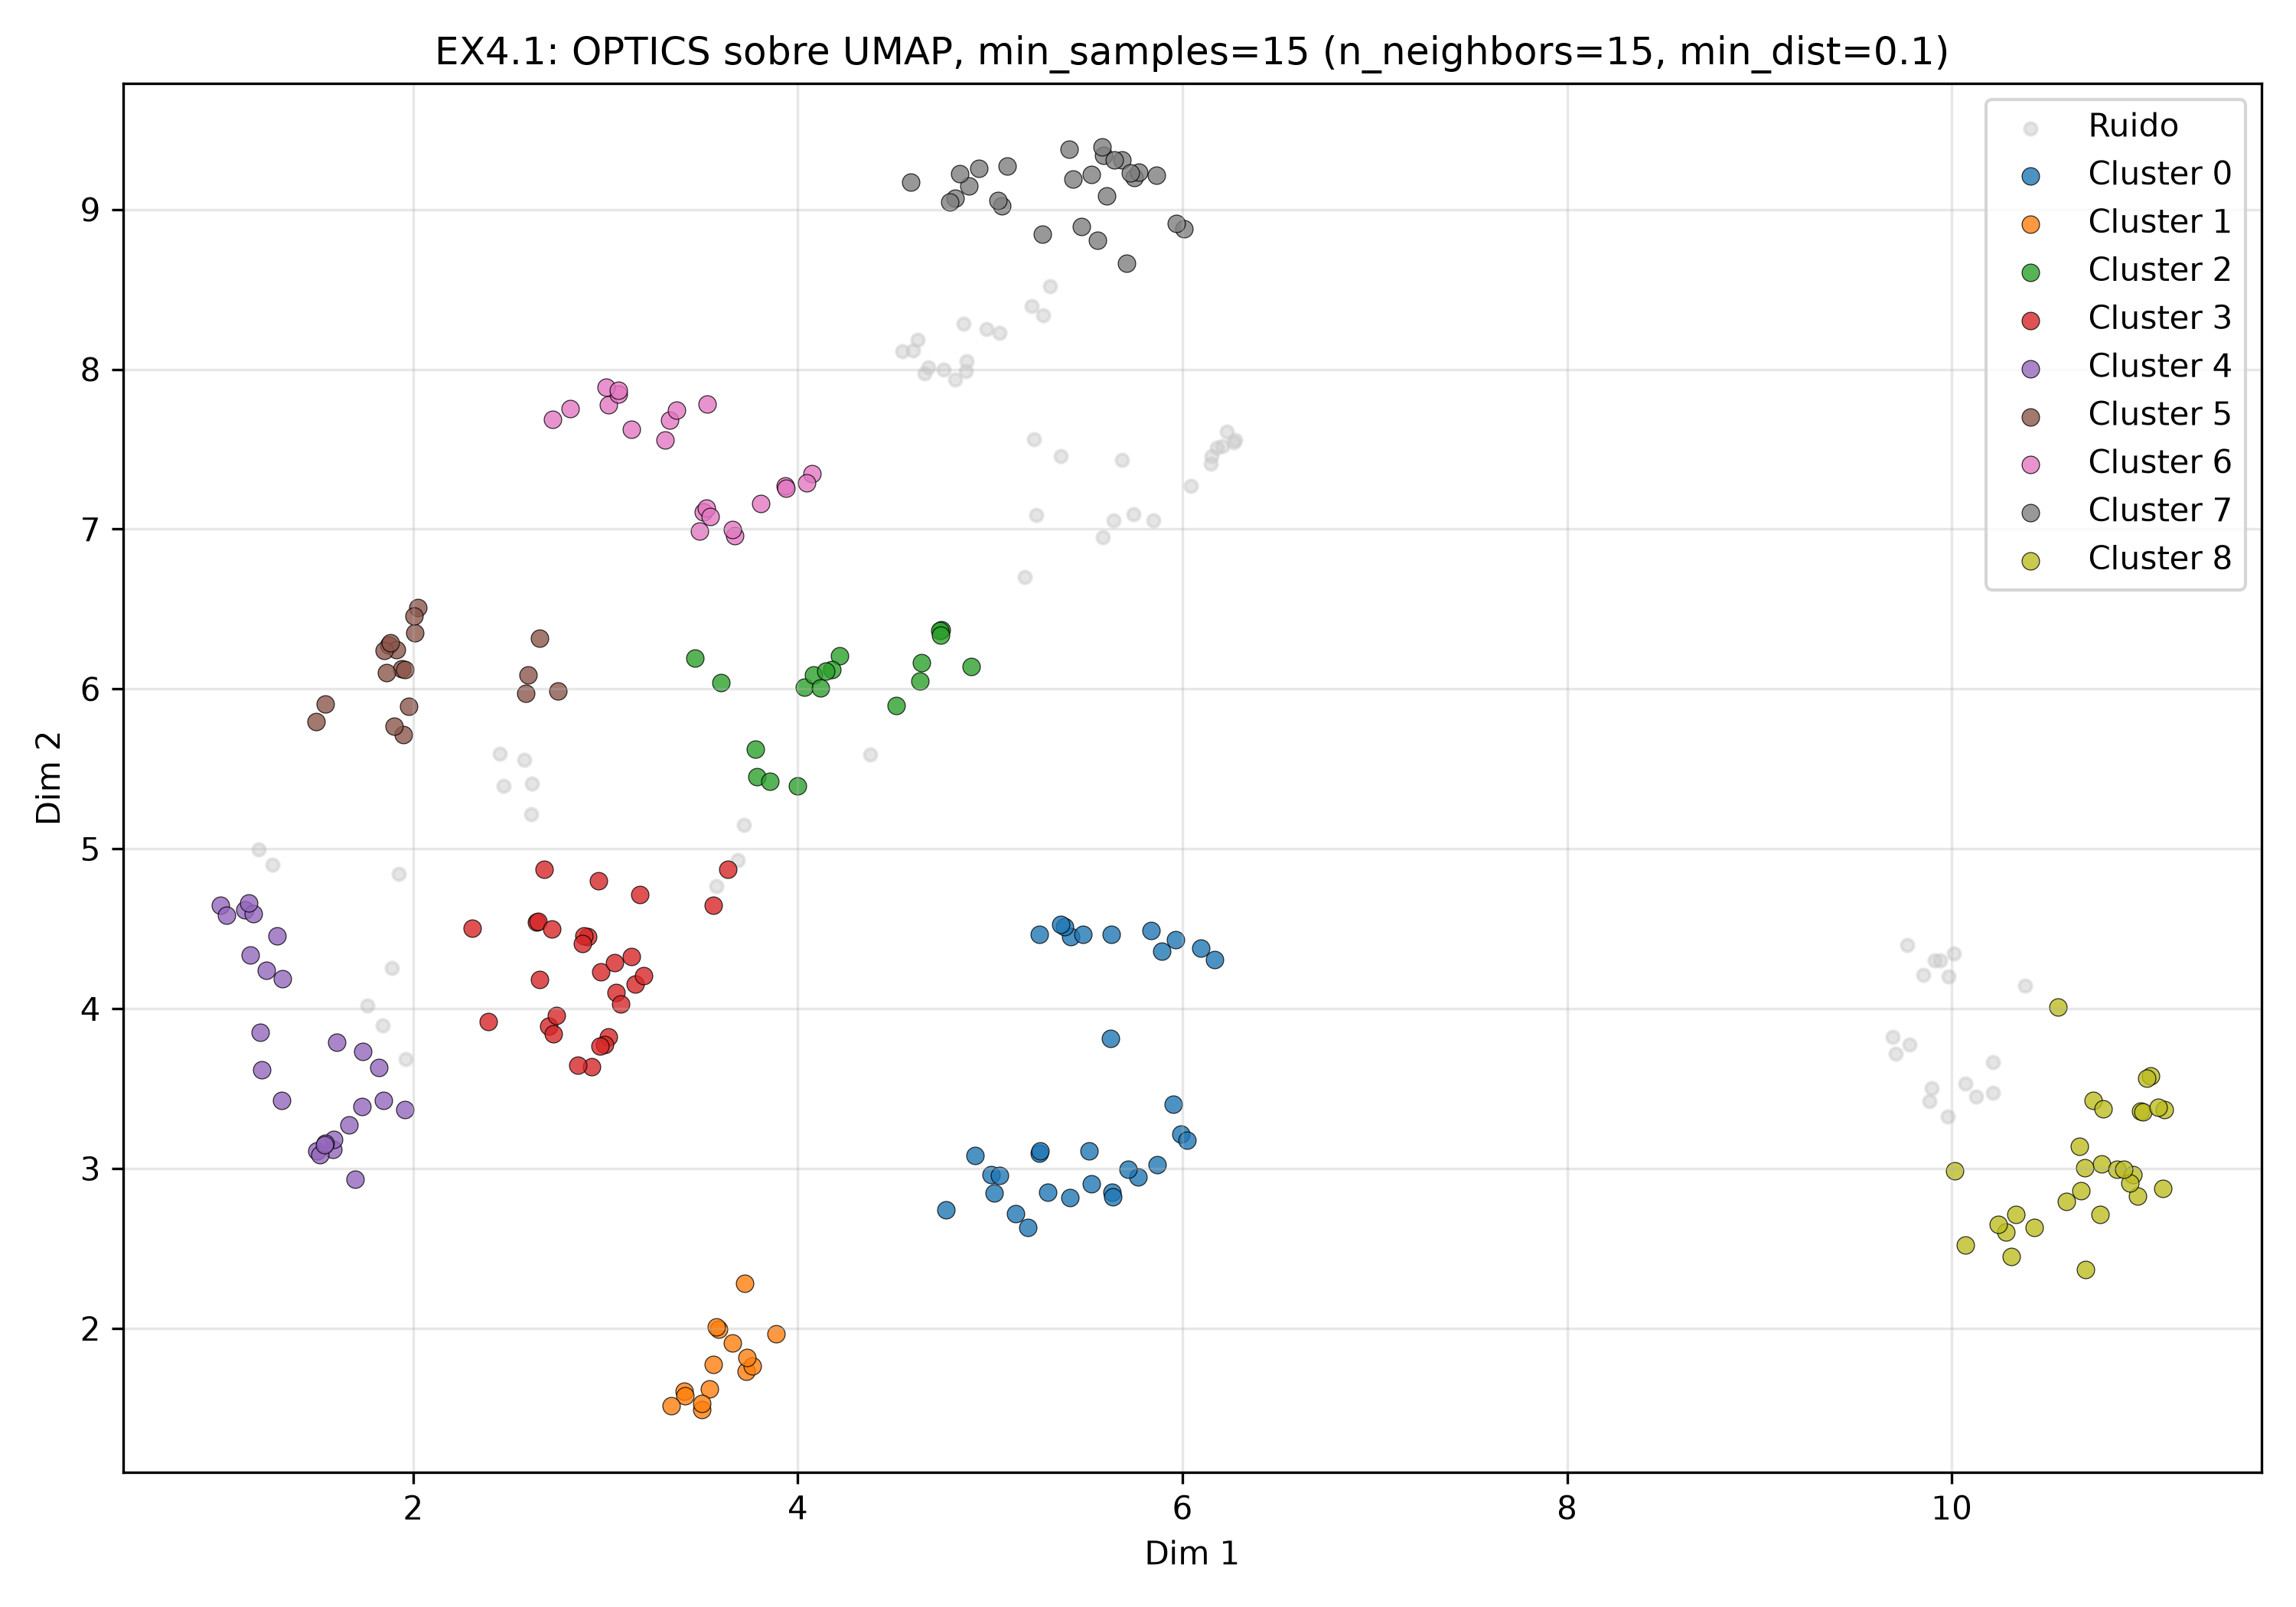
\includegraphics[width=\linewidth]{optics_umap_ms15.png}
    \caption{EX4.1: OPTICS sobre UMAP (ms=15).}
    \label{fig:optics_umap_ms15}
  \end{minipage}
\end{figure}

\begin{figure}[H]
  \centering
  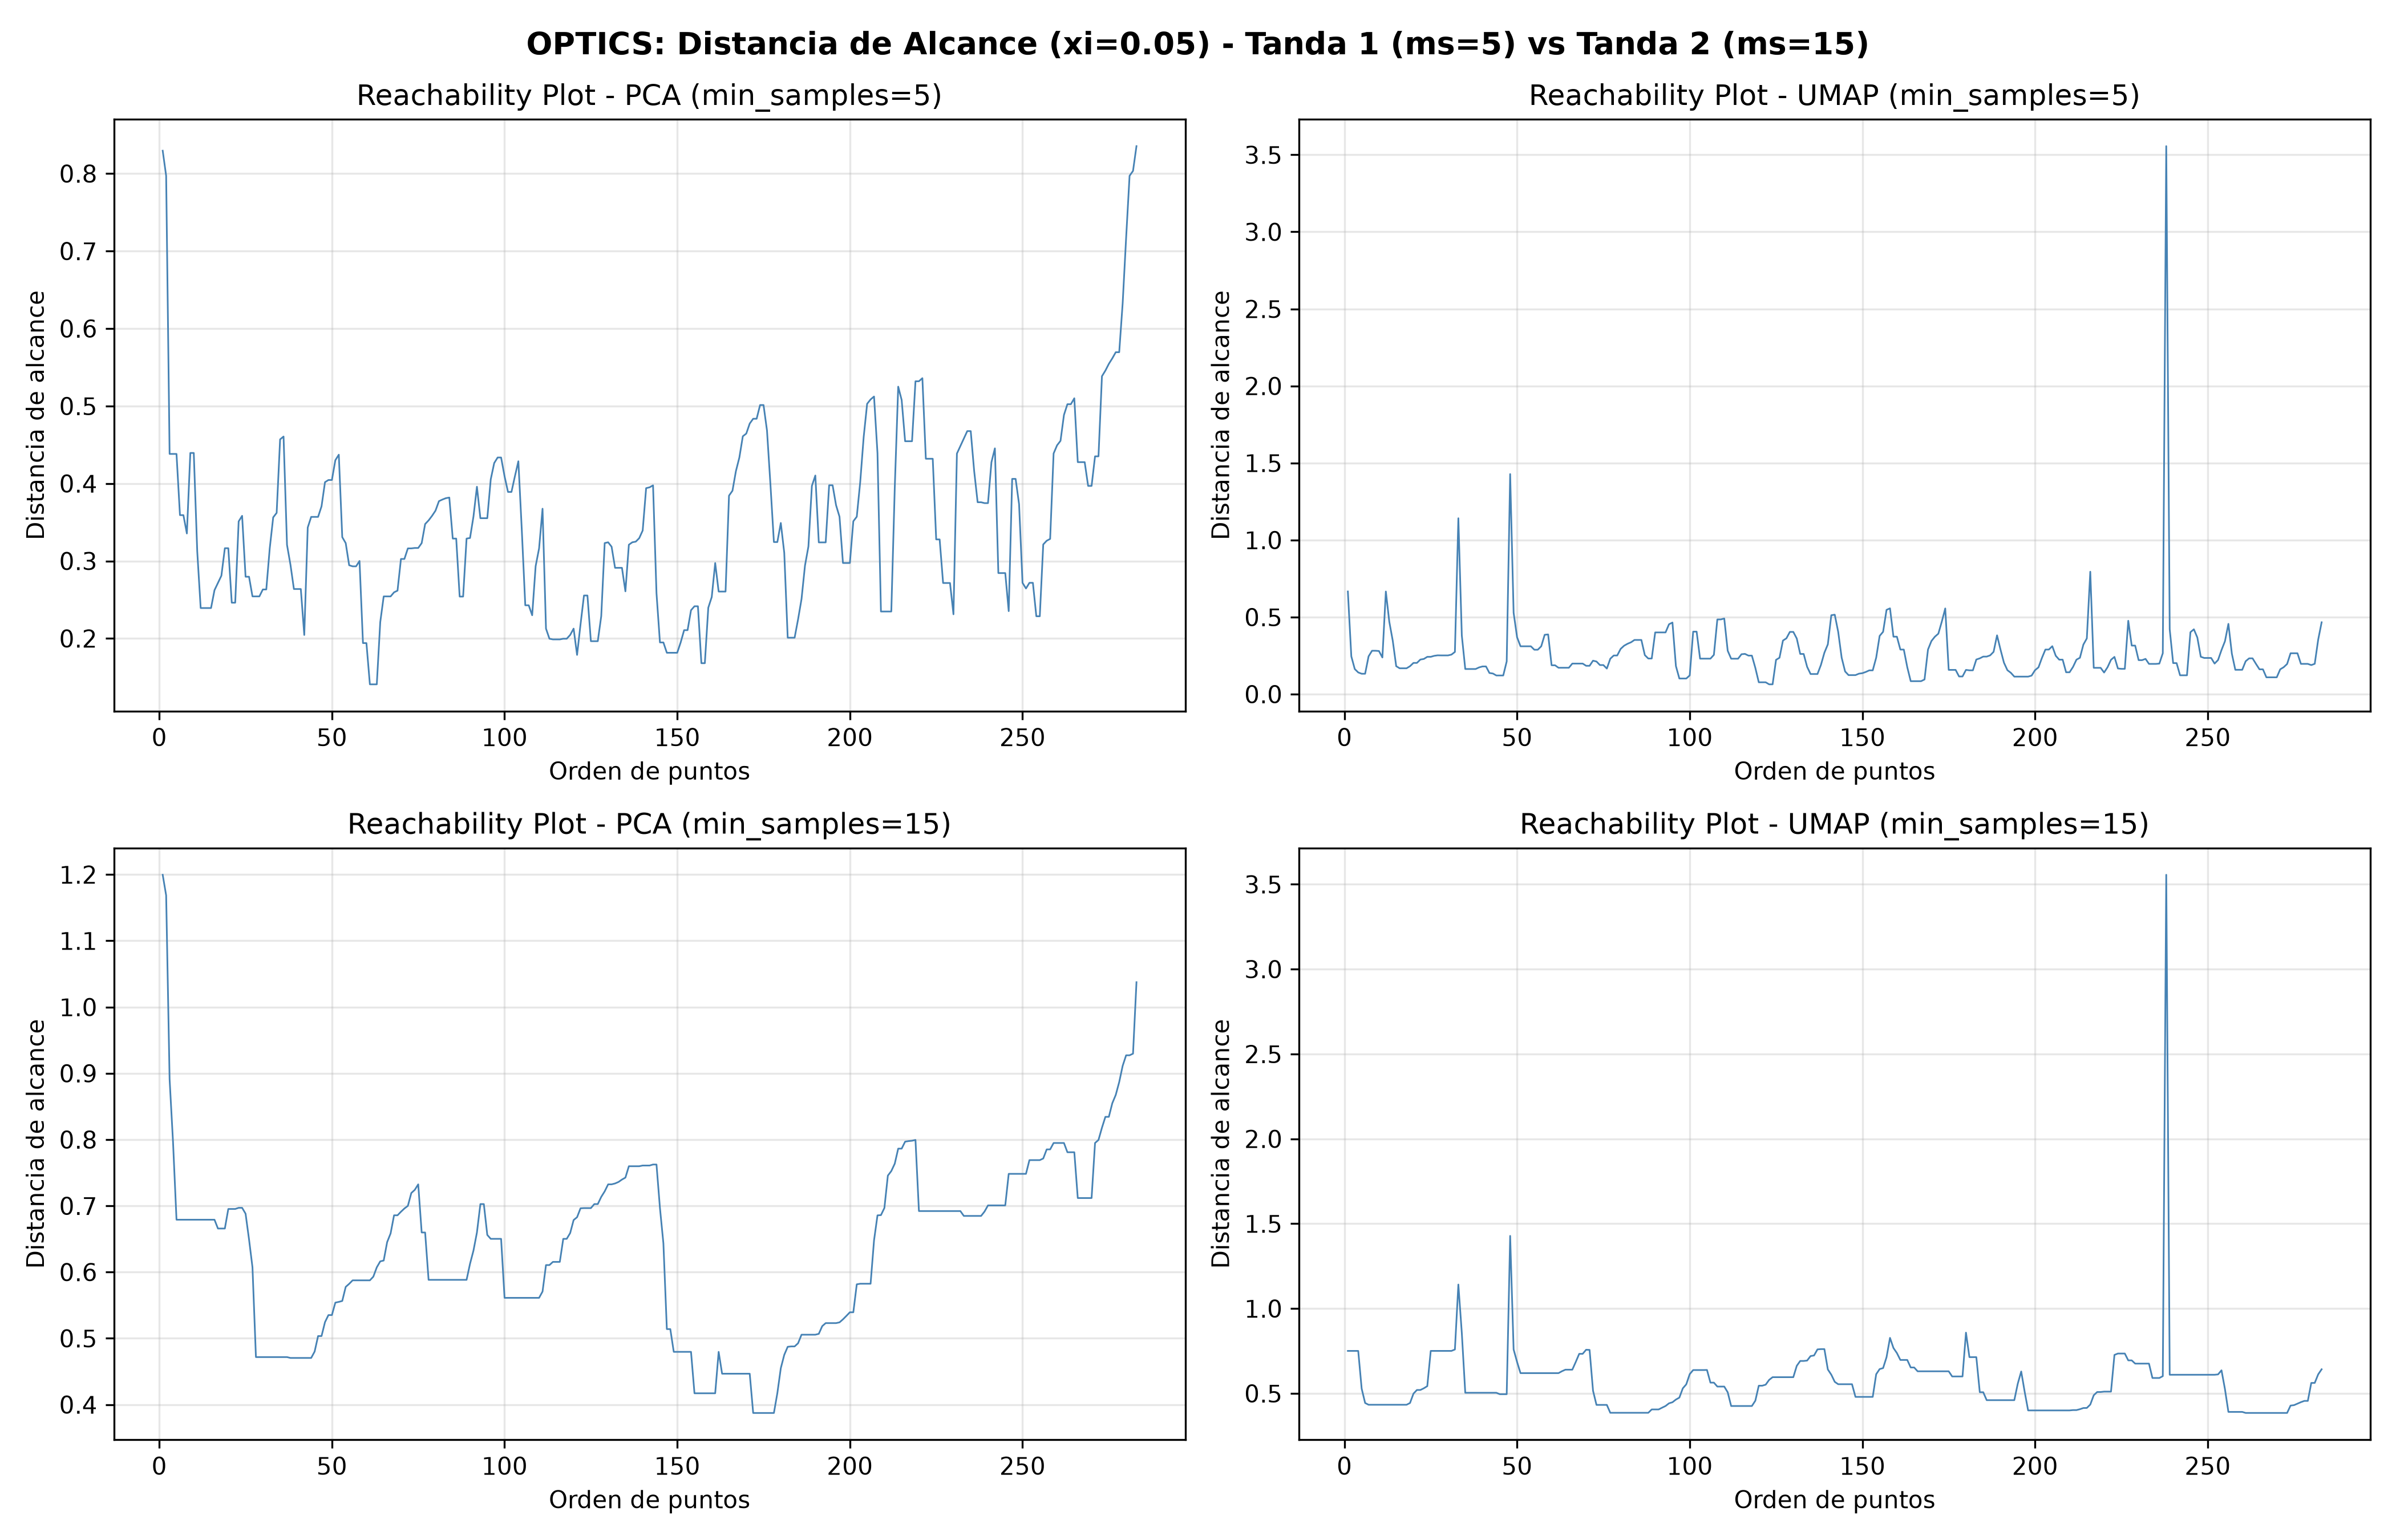
\includegraphics[width=0.85\linewidth]{optics_reachability.png}
  \caption{Reachability plots de OPTICS: tandas ms=5 y ms=15 sobre PCA y UMAP.}
  \label{fig:optics_reachability}
\end{figure}

\subsection{Evaluación}

\begin{figure}[H]
  \centering
  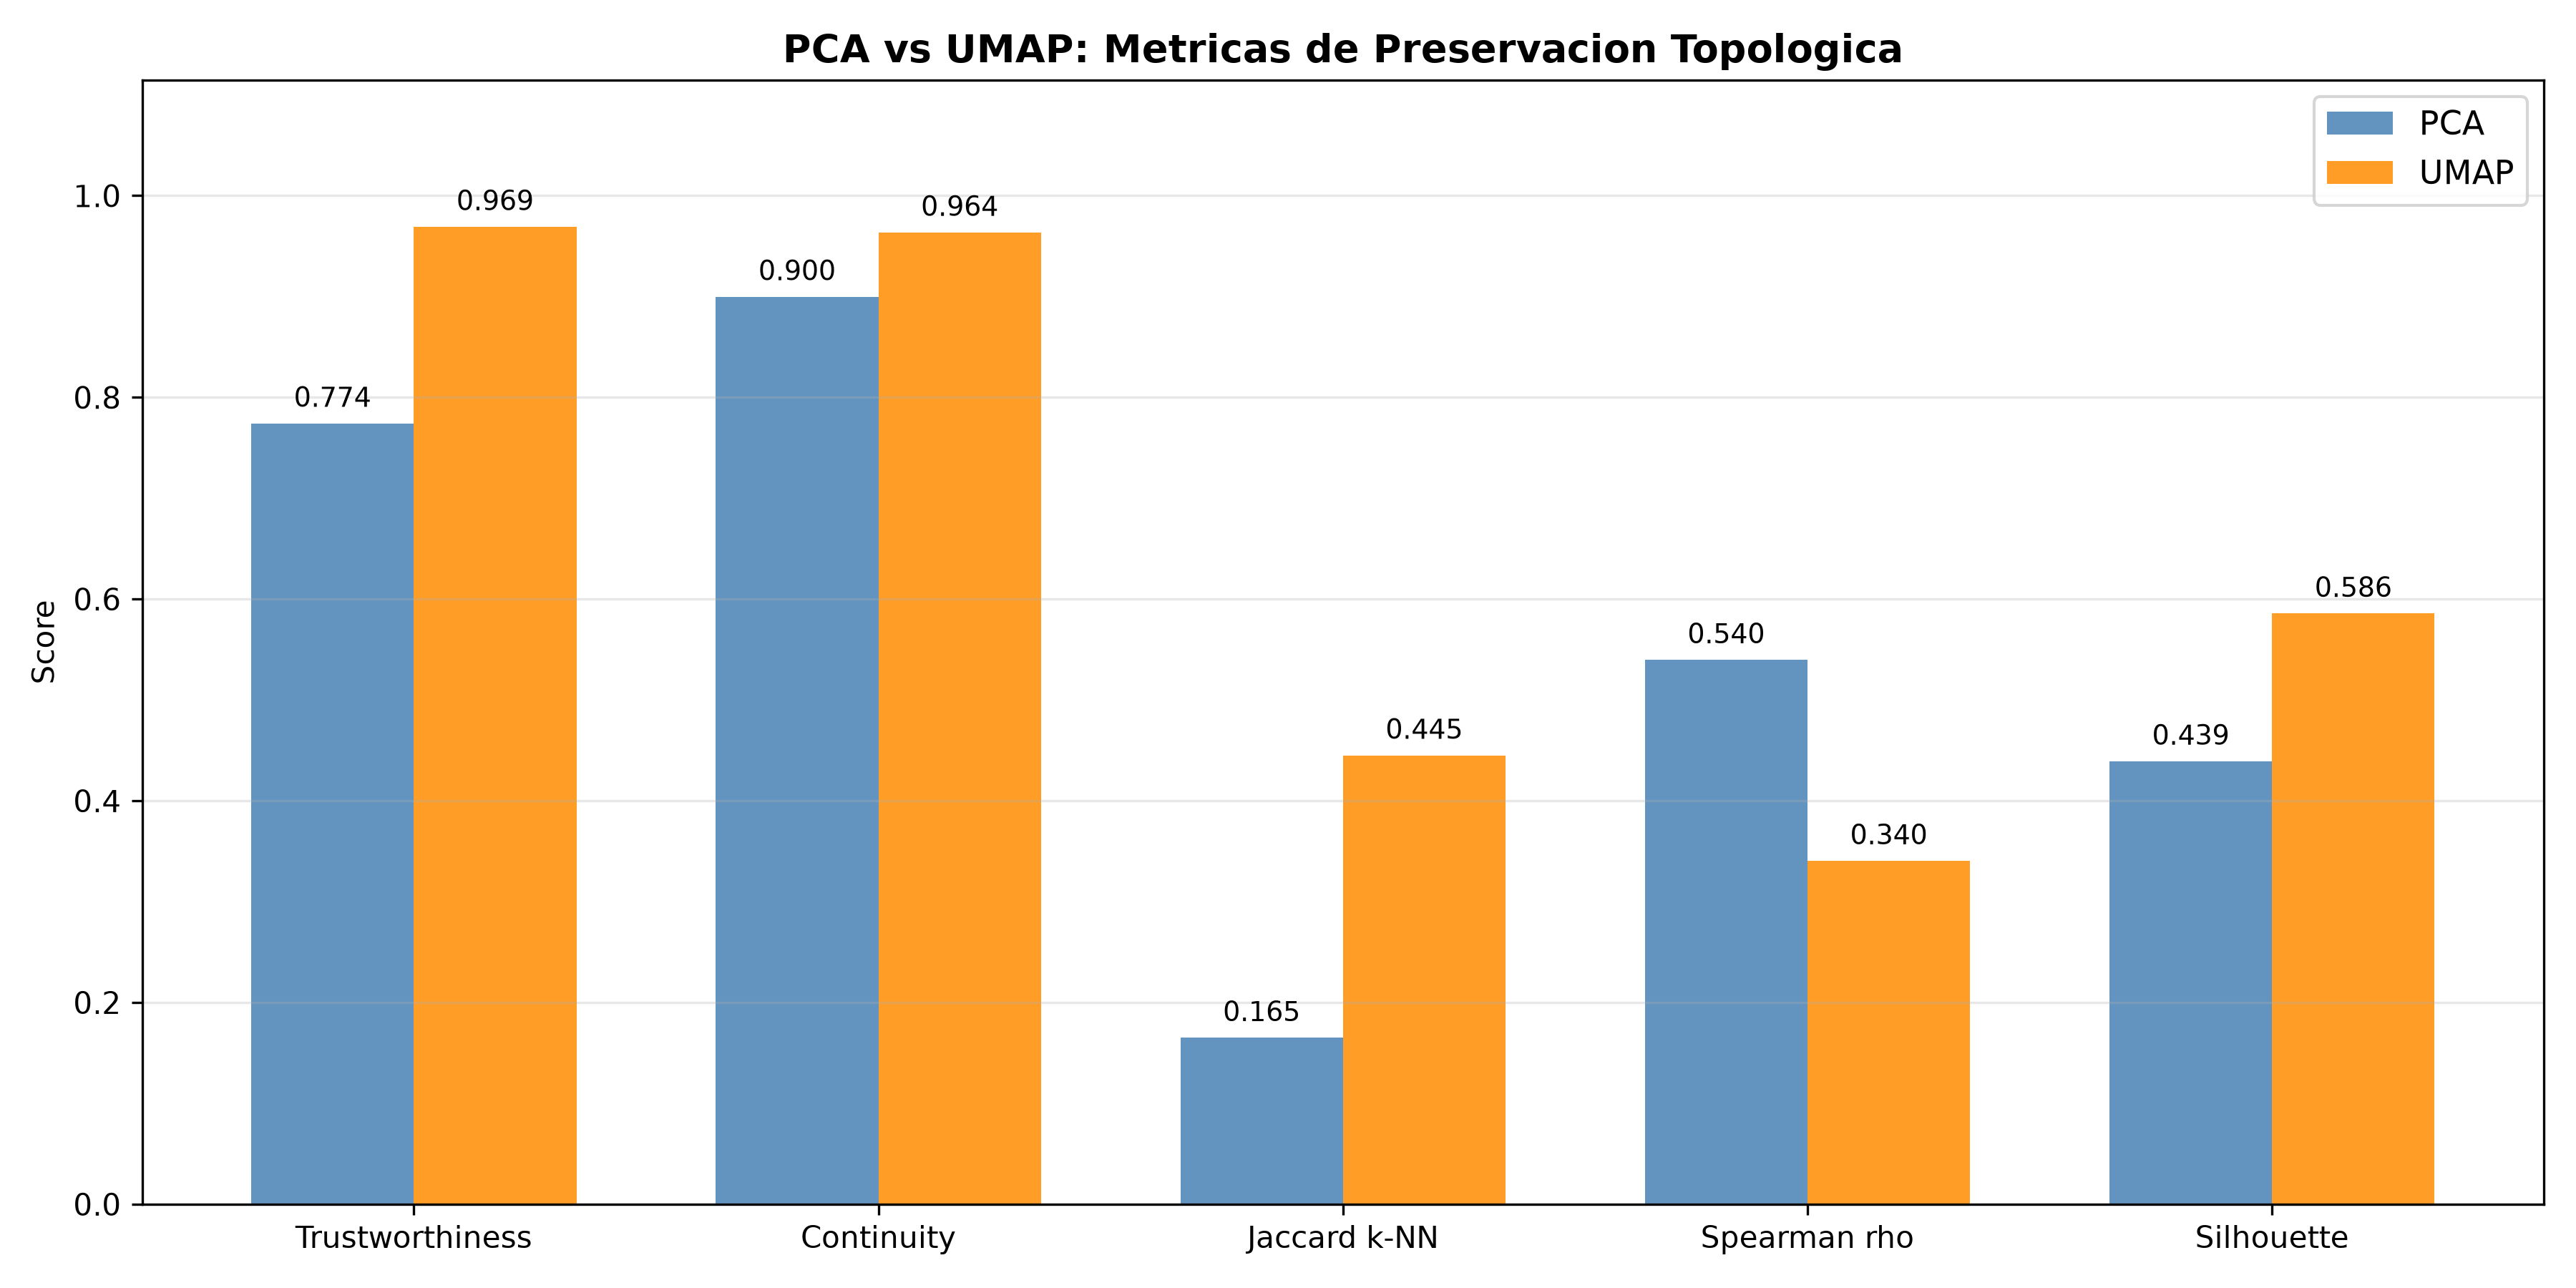
\includegraphics[width=0.85\linewidth]{pca_vs_umap_metrics.png}
  \caption{Métricas de preservación topológica: PCA vs. UMAP.}
  \label{fig:pca_vs_umap_metrics}
\end{figure}

\begin{figure}[H]
  \centering
  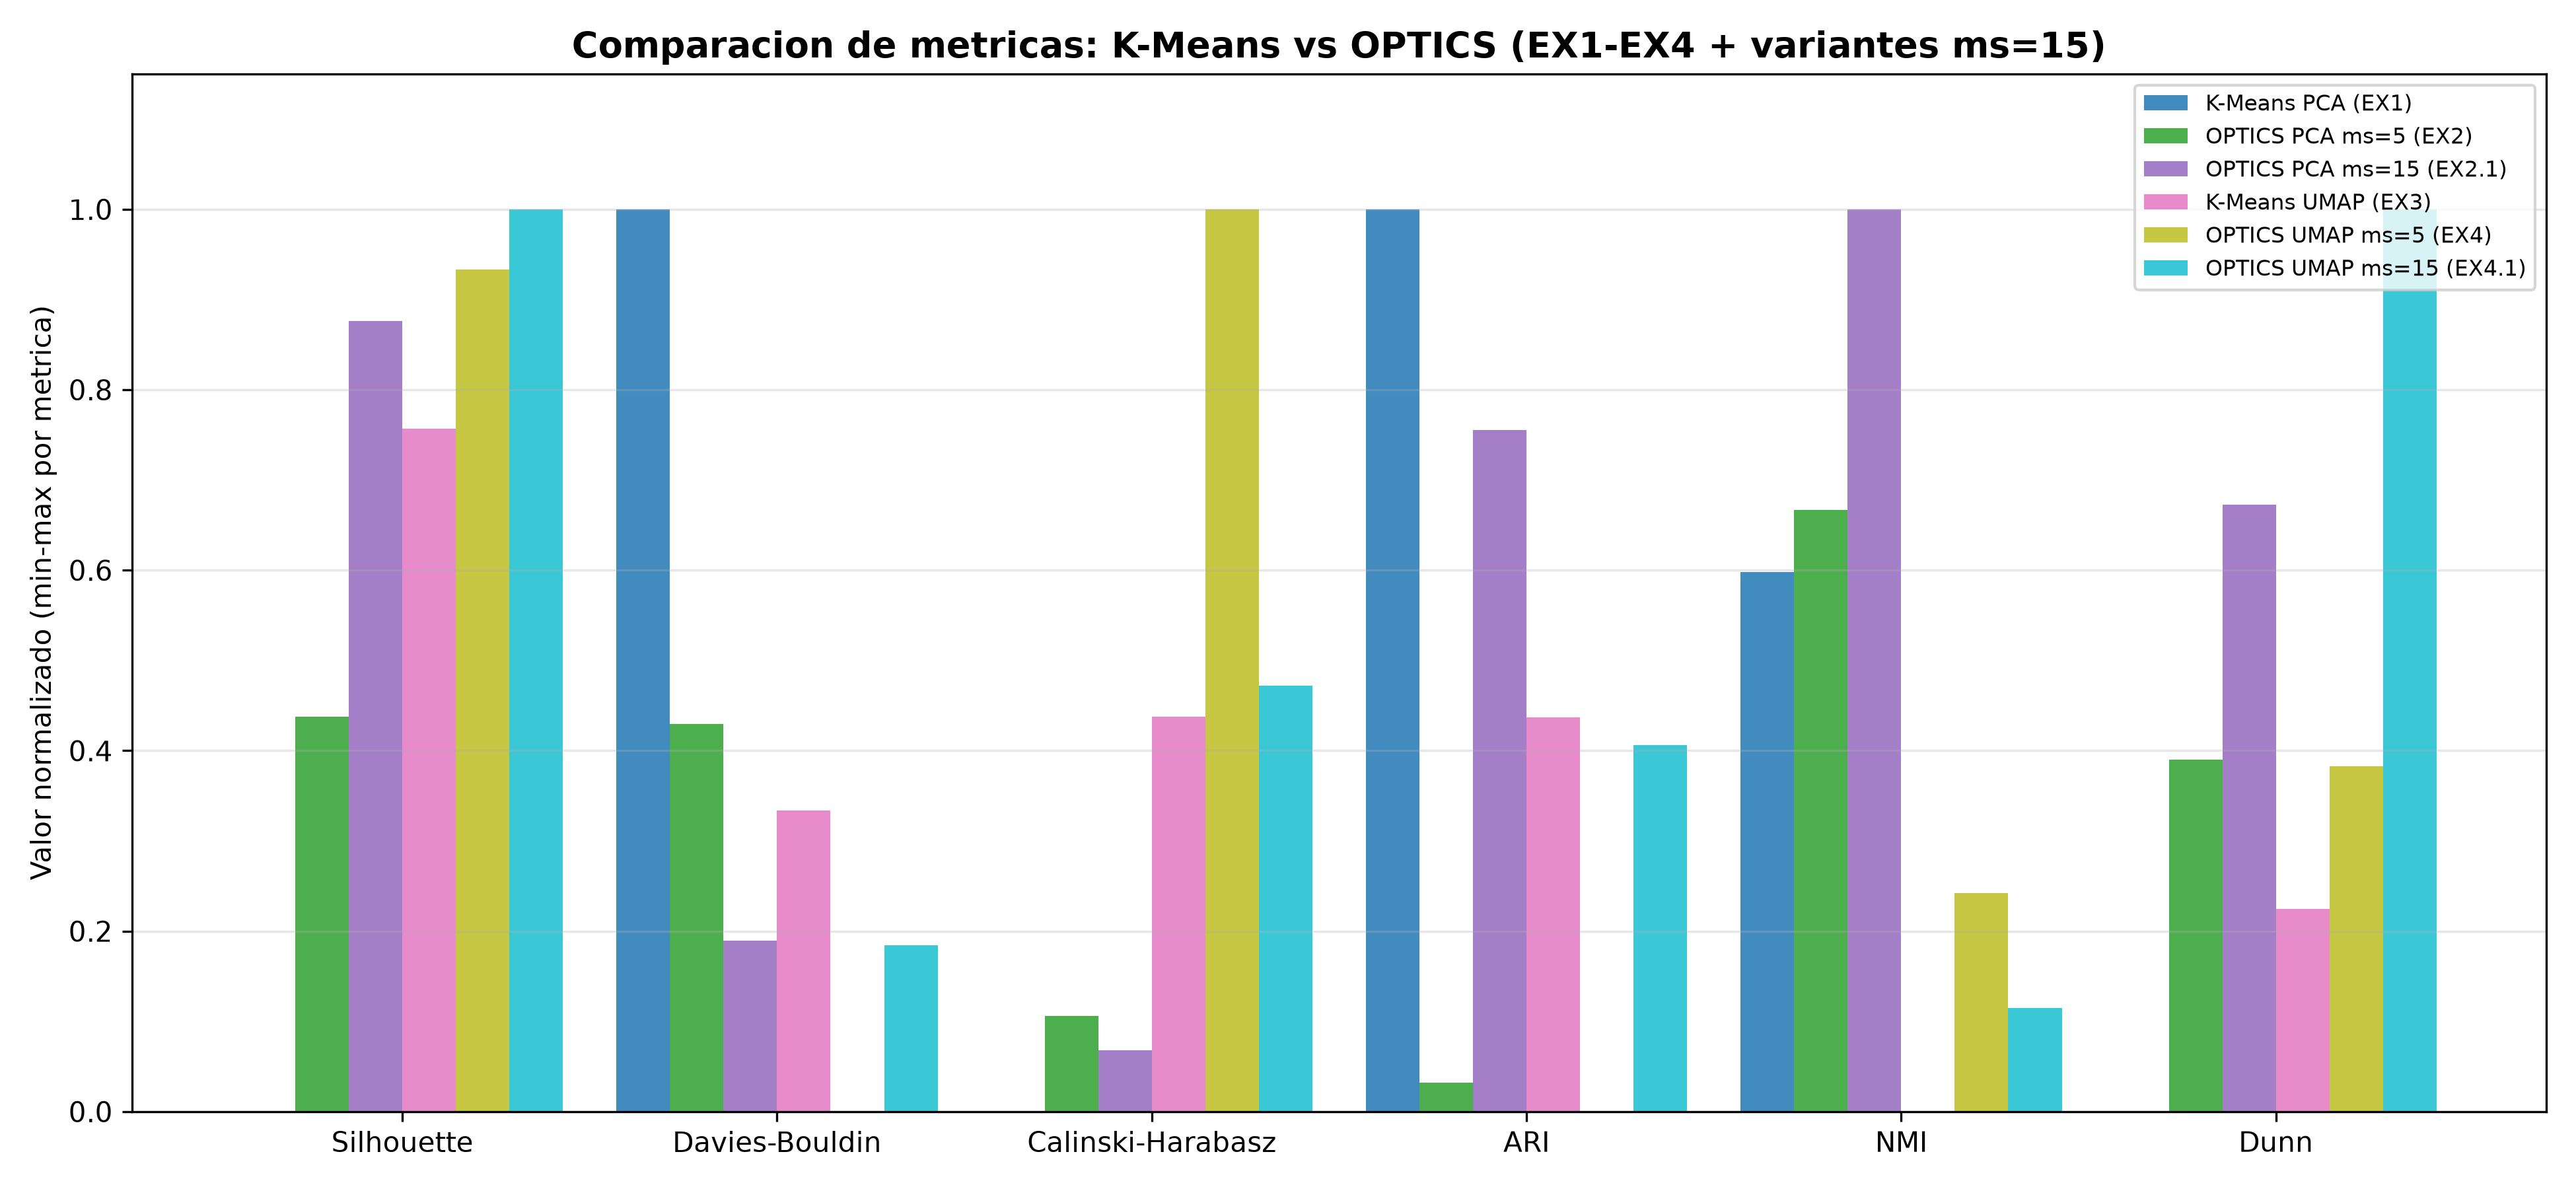
\includegraphics[width=\linewidth]{clustering_metrics.png}
  \caption{Comparación normalizada de métricas de clustering (EX1--EX4 + variantes ms=15).}
  \label{fig:clustering_metrics}
\end{figure}

% ============================================================
% 5. DISCUSIÓN
% ============================================================
\section{Discusión}\label{sec:discusion}

\subsection{PCA vs. UMAP}

PCA pierde efectividad en este dataset: retiene apenas el 29.5\,\% de la varianza en 2D y
requiere 11 de 22 componentes para el 80\,\%. Esto revela una estructura predominantemente no
lineal, terreno donde UMAP domina: gana en 4 de 5 métricas de preservación topológica, con
una ganancia notable en Jaccard k-NN (0.165 $\rightarrow$ 0.445) y trustworthiness
(0.774 $\rightarrow$ 0.969). La única métrica favorable a PCA es la correlación de Spearman
entre distancias, esperable porque PCA maximiza la preservación global. La interpretabilidad
es el punto a favor de PCA (la PC1 admite lectura clínica como ``indicador de salud
cardiaca''), mientras que los ejes de UMAP no tienen significado directo.

\subsection{K-Means vs. OPTICS}

Los modelos sobre UMAP superan sistemáticamente a los de PCA en todas las métricas de
compactidad: EX3 (0.618) supera a EX1 (0.447) en silueta, y lo mismo ocurre en OPTICS. Entre
algoritmos, OPTICS+UMAP (EX4.1, silueta 0.673 con 22.9\,\% de ruido) supera a K-Means+UMAP
(EX3, 0.618). Sin embargo, la comparación no es directa: la silueta de OPTICS se calcula
excluyendo el ruido, por lo que ``premia'' a los modelos que descartan más datos. En PCA con
\texttt{min\_samples=15} (EX2.1), el 70.1\,\% de los pacientes queda sin clasificar, lo que
invalida su utilidad clínica pese a su silueta de 0.645. El ruido de OPTICS es, por tanto, una
métrica tan importante como la silueta, y EX4.1 es el mejor equilibrio: máxima silueta con el
menor ruido de todas las variantes de densidad.

\subsection{Efecto de \texttt{min\_samples}}

Aumentar \texttt{min\_samples} de 5 a 15 reduce la fragmentación de clusters (20$\rightarrow$4
en PCA, 24$\rightarrow$9 en UMAP) y produce clusters más grandes y estables (tamaño mínimo
5$\rightarrow$15/18). En UMAP mejora tanto la silueta (0.658$\rightarrow$0.673) como el ruido
(29.6\,\%$\rightarrow$22.9\,\%), por lo que el aumento de exigencia de densidad beneficia a
la proyección que ya separa bien los grupos. En PCA ocurre lo contrario: el ruido sube a
70.1\,\%, evidencia de que la proyección lineal no concentra los grupos densos que OPTICS
busca.

\subsection{Validación externa}

El ARI es bajo en todos los modelos (máximo 0.177 en EX1), lo que indica que ningún
agrupamiento reproduce la severidad etiquetada (0--4). Esto era esperable: la severidad es
una escala ordinal clínica, no una partición geométrica ``natural'' de los datos. Aun así,
los perfiles de centroides de EX1 muestran coherencia clínica: el cluster 1 (jóvenes, FC alta,
ST normal) es 92\,\% sano, mientras el cluster 0 (mayores, FC baja, ST deprimida) es 86\,\%
enfermo. Los clusters descubren, por tanto, perfiles de riesgo plausibles más que réplicas
exactas del diagnóstico.

\subsection{Limitaciones}

\begin{itemize}
  \item \textbf{Muestra}: 284 registros es reducido para clustering por densidad; los
        resultados pueden no generalizar.
  \item \textbf{2D por visualización}: la proyección 2D descarta información (70.5\,\% en
        PCA); se priorizó la interpretabilidad gráfica.
  \item \textbf{UMAP estocástico}: depende de la semilla fijada (\texttt{random\_state=42}).
  \item \textbf{Métricas con ruido excluido}: la silueta de OPTICS no penaliza el porcentaje
        de datos descartados; se reporta el ruido por separado para mitigar este sesgo.
  \item \textbf{Ground truth ordinal}: el uso de ARI/NMI contra severidad 0--4 es
        conservador; una validación binaria (sano vs. enfermo) podría ser más informativa.
\end{itemize}

% ============================================================
% 6. CONCLUSIONES
% ============================================================
\section{Conclusiones}\label{sec:conclusiones}

\begin{enumerate}
  \item \textbf{Estructura no lineal}: el dataset requiere 11/22 componentes de PCA para el
        80\,\% de varianza, lo que evidencia una estructura mayoritariamente no lineal y
        justifica el uso de UMAP, que gana en 4 de 5 métricas de preservación topológica.
  \item \textbf{UMAP mejora el clustering}: tanto K-Means como OPTICS obtienen clusters más
        compactos sobre UMAP que sobre PCA, en todas las métricas internas evaluadas.
  \item \textbf{OPTICS es superior en calidad de agrupamiento, con matices}: EX4.1 (UMAP +
        OPTICS, \texttt{min\_samples=15}) logra la mejor silueta (0.673) y el menor ruido
        (22.9\,\%) de las variantes de densidad; la exclusión del ruido en la silueta exige
        reportar ambos indicadores para una lectura honesta.
  \item \textbf{Sensibilidad a \texttt{min\_samples}}: valores mayores reducen la
        fragmentación y, sobre UMAP, mejoran simultáneamente silueta y ruido; sobre PCA
        degradan la cobertura (70.1\,\% de ruido en EX2.1).
  \item \textbf{Los clusters no replican la severidad}: el ARI máximo es 0.177; los
        agrupamientos describen perfiles clínicos alternativos (p.~ej., el cluster sano de
        EX1 es 92\,\% severidad 0 y el cluster crítico es 86\,\% severidad 1--4), que
        responden a las preguntas de análisis: sí existen grupos naturales, UMAP los separa
        mejor, y las variables que más influyen son las asociadas al segmento ST
        (\texttt{oldpeak}, \texttt{slope}), la FC máxima (\texttt{thalach}) y el talio
        (\texttt{thal}).
  \item \textbf{Cumplimiento del plan}: se ejecutaron las etapas KDD planificadas, con una
        desviación documentada (DBSCAN $\rightarrow$ OPTICS) y una extensión de
        sensibilidad de \texttt{min\_samples}, todo reproducible desde el notebook
        \cite{notebook} y el script consolidado \cite{script}.
\end{enumerate}

Como trabajo futuro se propone explorar proyecciones 3D, probar t-SNE y modelos de mezcla
gaussianos, y redefinir la validación externa en términos binarios (sano vs. enfermo).

% ============================================================
% 7. REFERENCIAS
% ============================================================
\begin{thebibliography}{99}\label{sec:referencias}

\bibitem{planificacion}
Grupo ADD (2026). \emph{Planificación del Proyecto Semestral: Análisis con Reducción de
Dimensionalidad y Clustering}. Documento del proyecto, \texttt{Planificacion/ADD\_V2\_Final.pdf}.

\bibitem{notebook}
Grupo ADD (2026). \emph{proyecto-add-1-2026\_ejecutado.ipynb}. Notebook ejecutado del
proyecto (Jupyter/Colab).

\bibitem{script}
Grupo ADD (2026). \emph{analisis\_consolidado.py}. Script consolidado del pipeline de análisis.

\bibitem{presentacion}
Grupo ADD (2026). \emph{presentacion.tex}. Presentación del proyecto (Beamer/LaTeX).

\bibitem{detrano1989}
Detrano, R., Jánosi, A., Steinbrunn, W., Pfisterer, M., Schmid, J., Sandhu, S., Guppy, K.,
Lee, S., \& Froelicher, V. (1989). International application of a new probability algorithm
for the diagnosis of coronary artery disease. \emph{American Journal of Cardiology}, 64(5),
304--310.

\bibitem{pearson1901}
Pearson, K. (1901). On lines and planes of closest fit to systems of points in space.
\emph{Philosophical Magazine}, 2(11), 559--572.

\bibitem{hotelling1933}
Hotelling, H. (1933). Analysis of a complex of statistical variables into principal
components. \emph{Journal of Educational Psychology}, 24(6), 417--441.

\bibitem{kaiser1960}
Kaiser, H. F. (1960). The application of electronic computers to factor analysis.
\emph{Educational and Psychological Measurement}, 20(1), 141--151.

\bibitem{cattell1966}
Cattell, R. B. (1966). The scree test for the number of factors. \emph{Multivariate
Behavioral Research}, 1(2), 245--276.

\bibitem{mcinnes2018}
McInnes, L., Healy, J., \& Melville, J. (2018). UMAP: Uniform Manifold Approximation and
Projection for Dimension Reduction. \emph{arXiv preprint arXiv:1802.03426}.

\bibitem{lloyd1982}
Lloyd, S. P. (1982). Least squares quantization in PCM. \emph{IEEE Transactions on
Information Theory}, 28(2), 129--137.

\bibitem{macqueen1967}
MacQueen, J. (1967). Some methods for classification and analysis of multivariate
observations. \emph{Proceedings of the 5th Berkeley Symposium on Mathematical Statistics and
Probability}, 1, 281--297.

\bibitem{ankerst1999}
Ankerst, M., Breunig, M. M., Kriegel, H.-P., \& Sander, J. (1999). OPTICS: Ordering points
to identify the clustering structure. \emph{ACM SIGMOD Record}, 28(2), 49--60.

\bibitem{rousseeuw1987}
Rousseeuw, P. J. (1987). Silhouettes: A graphical aid to the interpretation and validation
of cluster analysis. \emph{Journal of Computational and Applied Mathematics}, 20, 53--65.

\bibitem{davies1979}
Davies, D. L., \& Bouldin, D. W. (1979). A cluster separation measure. \emph{IEEE
Transactions on Pattern Analysis and Machine Intelligence}, PAMI-1(2), 224--227.

\bibitem{calinski1974}
Calinski, T., \& Harabasz, J. (1974). A dendrite method for cluster analysis.
\emph{Communications in Statistics}, 3(1), 1--27.

\bibitem{hubert1985}
Hubert, L., \& Arabie, P. (1985). Comparing partitions. \emph{Journal of Classification},
2(1), 193--218.

\bibitem{dunn1974}
Dunn, J. C. (1974). Well-separated clusters and optimal fuzzy partitions. \emph{Journal of
Cybernetics}, 4(1), 95--104.

\bibitem{lee2009}
Lee, J. A., \& Verleysen, M. (2009). Quality assessment of dimensionality reduction:
Rank-based criteria. \emph{Neurocomputing}, 72(7--9), 1431--1443.

\bibitem{uci}
UCI Machine Learning Repository. Heart Disease Dataset. Disponible en
\url{https://archive.ics.uci.edu/dataset/45/heart+disease}.

\end{thebibliography}

\end{document}
